% Options for packages loaded elsewhere
\PassOptionsToPackage{unicode}{hyperref}
\PassOptionsToPackage{hyphens}{url}
\PassOptionsToPackage{dvipsnames,svgnames,x11names}{xcolor}
%
\documentclass[
  letterpaper,
  DIV=11,
  numbers=noendperiod]{scrreprt}

\usepackage{amsmath,amssymb}
\usepackage{lmodern}
\usepackage{iftex}
\ifPDFTeX
  \usepackage[T1]{fontenc}
  \usepackage[utf8]{inputenc}
  \usepackage{textcomp} % provide euro and other symbols
\else % if luatex or xetex
  \usepackage{unicode-math}
  \defaultfontfeatures{Scale=MatchLowercase}
  \defaultfontfeatures[\rmfamily]{Ligatures=TeX,Scale=1}
\fi
% Use upquote if available, for straight quotes in verbatim environments
\IfFileExists{upquote.sty}{\usepackage{upquote}}{}
\IfFileExists{microtype.sty}{% use microtype if available
  \usepackage[]{microtype}
  \UseMicrotypeSet[protrusion]{basicmath} % disable protrusion for tt fonts
}{}
\makeatletter
\@ifundefined{KOMAClassName}{% if non-KOMA class
  \IfFileExists{parskip.sty}{%
    \usepackage{parskip}
  }{% else
    \setlength{\parindent}{0pt}
    \setlength{\parskip}{6pt plus 2pt minus 1pt}}
}{% if KOMA class
  \KOMAoptions{parskip=half}}
\makeatother
\usepackage{xcolor}
\setlength{\emergencystretch}{3em} % prevent overfull lines
\setcounter{secnumdepth}{5}
% Make \paragraph and \subparagraph free-standing
\ifx\paragraph\undefined\else
  \let\oldparagraph\paragraph
  \renewcommand{\paragraph}[1]{\oldparagraph{#1}\mbox{}}
\fi
\ifx\subparagraph\undefined\else
  \let\oldsubparagraph\subparagraph
  \renewcommand{\subparagraph}[1]{\oldsubparagraph{#1}\mbox{}}
\fi

\usepackage{color}
\usepackage{fancyvrb}
\newcommand{\VerbBar}{|}
\newcommand{\VERB}{\Verb[commandchars=\\\{\}]}
\DefineVerbatimEnvironment{Highlighting}{Verbatim}{commandchars=\\\{\}}
% Add ',fontsize=\small' for more characters per line
\usepackage{framed}
\definecolor{shadecolor}{RGB}{241,243,245}
\newenvironment{Shaded}{\begin{snugshade}}{\end{snugshade}}
\newcommand{\AlertTok}[1]{\textcolor[rgb]{0.68,0.00,0.00}{#1}}
\newcommand{\AnnotationTok}[1]{\textcolor[rgb]{0.37,0.37,0.37}{#1}}
\newcommand{\AttributeTok}[1]{\textcolor[rgb]{0.40,0.45,0.13}{#1}}
\newcommand{\BaseNTok}[1]{\textcolor[rgb]{0.68,0.00,0.00}{#1}}
\newcommand{\BuiltInTok}[1]{\textcolor[rgb]{0.00,0.23,0.31}{#1}}
\newcommand{\CharTok}[1]{\textcolor[rgb]{0.13,0.47,0.30}{#1}}
\newcommand{\CommentTok}[1]{\textcolor[rgb]{0.37,0.37,0.37}{#1}}
\newcommand{\CommentVarTok}[1]{\textcolor[rgb]{0.37,0.37,0.37}{\textit{#1}}}
\newcommand{\ConstantTok}[1]{\textcolor[rgb]{0.56,0.35,0.01}{#1}}
\newcommand{\ControlFlowTok}[1]{\textcolor[rgb]{0.00,0.23,0.31}{#1}}
\newcommand{\DataTypeTok}[1]{\textcolor[rgb]{0.68,0.00,0.00}{#1}}
\newcommand{\DecValTok}[1]{\textcolor[rgb]{0.68,0.00,0.00}{#1}}
\newcommand{\DocumentationTok}[1]{\textcolor[rgb]{0.37,0.37,0.37}{\textit{#1}}}
\newcommand{\ErrorTok}[1]{\textcolor[rgb]{0.68,0.00,0.00}{#1}}
\newcommand{\ExtensionTok}[1]{\textcolor[rgb]{0.00,0.23,0.31}{#1}}
\newcommand{\FloatTok}[1]{\textcolor[rgb]{0.68,0.00,0.00}{#1}}
\newcommand{\FunctionTok}[1]{\textcolor[rgb]{0.28,0.35,0.67}{#1}}
\newcommand{\ImportTok}[1]{\textcolor[rgb]{0.00,0.46,0.62}{#1}}
\newcommand{\InformationTok}[1]{\textcolor[rgb]{0.37,0.37,0.37}{#1}}
\newcommand{\KeywordTok}[1]{\textcolor[rgb]{0.00,0.23,0.31}{#1}}
\newcommand{\NormalTok}[1]{\textcolor[rgb]{0.00,0.23,0.31}{#1}}
\newcommand{\OperatorTok}[1]{\textcolor[rgb]{0.37,0.37,0.37}{#1}}
\newcommand{\OtherTok}[1]{\textcolor[rgb]{0.00,0.23,0.31}{#1}}
\newcommand{\PreprocessorTok}[1]{\textcolor[rgb]{0.68,0.00,0.00}{#1}}
\newcommand{\RegionMarkerTok}[1]{\textcolor[rgb]{0.00,0.23,0.31}{#1}}
\newcommand{\SpecialCharTok}[1]{\textcolor[rgb]{0.37,0.37,0.37}{#1}}
\newcommand{\SpecialStringTok}[1]{\textcolor[rgb]{0.13,0.47,0.30}{#1}}
\newcommand{\StringTok}[1]{\textcolor[rgb]{0.13,0.47,0.30}{#1}}
\newcommand{\VariableTok}[1]{\textcolor[rgb]{0.07,0.07,0.07}{#1}}
\newcommand{\VerbatimStringTok}[1]{\textcolor[rgb]{0.13,0.47,0.30}{#1}}
\newcommand{\WarningTok}[1]{\textcolor[rgb]{0.37,0.37,0.37}{\textit{#1}}}

\providecommand{\tightlist}{%
  \setlength{\itemsep}{0pt}\setlength{\parskip}{0pt}}\usepackage{longtable,booktabs,array}
\usepackage{calc} % for calculating minipage widths
% Correct order of tables after \paragraph or \subparagraph
\usepackage{etoolbox}
\makeatletter
\patchcmd\longtable{\par}{\if@noskipsec\mbox{}\fi\par}{}{}
\makeatother
% Allow footnotes in longtable head/foot
\IfFileExists{footnotehyper.sty}{\usepackage{footnotehyper}}{\usepackage{footnote}}
\makesavenoteenv{longtable}
\usepackage{graphicx}
\makeatletter
\def\maxwidth{\ifdim\Gin@nat@width>\linewidth\linewidth\else\Gin@nat@width\fi}
\def\maxheight{\ifdim\Gin@nat@height>\textheight\textheight\else\Gin@nat@height\fi}
\makeatother
% Scale images if necessary, so that they will not overflow the page
% margins by default, and it is still possible to overwrite the defaults
% using explicit options in \includegraphics[width, height, ...]{}
\setkeys{Gin}{width=\maxwidth,height=\maxheight,keepaspectratio}
% Set default figure placement to htbp
\makeatletter
\def\fps@figure{htbp}
\makeatother
\newlength{\cslhangindent}
\setlength{\cslhangindent}{1.5em}
\newlength{\csllabelwidth}
\setlength{\csllabelwidth}{3em}
\newlength{\cslentryspacingunit} % times entry-spacing
\setlength{\cslentryspacingunit}{\parskip}
\newenvironment{CSLReferences}[2] % #1 hanging-ident, #2 entry spacing
 {% don't indent paragraphs
  \setlength{\parindent}{0pt}
  % turn on hanging indent if param 1 is 1
  \ifodd #1
  \let\oldpar\par
  \def\par{\hangindent=\cslhangindent\oldpar}
  \fi
  % set entry spacing
  \setlength{\parskip}{#2\cslentryspacingunit}
 }%
 {}
\usepackage{calc}
\newcommand{\CSLBlock}[1]{#1\hfill\break}
\newcommand{\CSLLeftMargin}[1]{\parbox[t]{\csllabelwidth}{#1}}
\newcommand{\CSLRightInline}[1]{\parbox[t]{\linewidth - \csllabelwidth}{#1}\break}
\newcommand{\CSLIndent}[1]{\hspace{\cslhangindent}#1}

\usepackage{makeidx}
\makeindex
\KOMAoption{captions}{tableheading}
\makeatletter
\@ifpackageloaded{tcolorbox}{}{\usepackage[many]{tcolorbox}}
\@ifpackageloaded{fontawesome5}{}{\usepackage{fontawesome5}}
\definecolor{quarto-callout-color}{HTML}{909090}
\definecolor{quarto-callout-note-color}{HTML}{0758E5}
\definecolor{quarto-callout-important-color}{HTML}{CC1914}
\definecolor{quarto-callout-warning-color}{HTML}{EB9113}
\definecolor{quarto-callout-tip-color}{HTML}{00A047}
\definecolor{quarto-callout-caution-color}{HTML}{FC5300}
\definecolor{quarto-callout-color-frame}{HTML}{acacac}
\definecolor{quarto-callout-note-color-frame}{HTML}{4582ec}
\definecolor{quarto-callout-important-color-frame}{HTML}{d9534f}
\definecolor{quarto-callout-warning-color-frame}{HTML}{f0ad4e}
\definecolor{quarto-callout-tip-color-frame}{HTML}{02b875}
\definecolor{quarto-callout-caution-color-frame}{HTML}{fd7e14}
\makeatother
\makeatletter
\makeatother
\makeatletter
\@ifpackageloaded{bookmark}{}{\usepackage{bookmark}}
\makeatother
\makeatletter
\@ifpackageloaded{caption}{}{\usepackage{caption}}
\AtBeginDocument{%
\ifdefined\contentsname
  \renewcommand*\contentsname{Table of contents}
\else
  \newcommand\contentsname{Table of contents}
\fi
\ifdefined\listfigurename
  \renewcommand*\listfigurename{List of Figures}
\else
  \newcommand\listfigurename{List of Figures}
\fi
\ifdefined\listtablename
  \renewcommand*\listtablename{List of Tables}
\else
  \newcommand\listtablename{List of Tables}
\fi
\ifdefined\figurename
  \renewcommand*\figurename{Figure}
\else
  \newcommand\figurename{Figure}
\fi
\ifdefined\tablename
  \renewcommand*\tablename{Table}
\else
  \newcommand\tablename{Table}
\fi
}
\@ifpackageloaded{float}{}{\usepackage{float}}
\floatstyle{ruled}
\@ifundefined{c@chapter}{\newfloat{codelisting}{h}{lop}}{\newfloat{codelisting}{h}{lop}[chapter]}
\floatname{codelisting}{Listing}
\newcommand*\listoflistings{\listof{codelisting}{List of Listings}}
\makeatother
\makeatletter
\@ifpackageloaded{caption}{}{\usepackage{caption}}
\@ifpackageloaded{subcaption}{}{\usepackage{subcaption}}
\makeatother
\makeatletter
\@ifpackageloaded{tcolorbox}{}{\usepackage[many]{tcolorbox}}
\makeatother
\makeatletter
\@ifundefined{shadecolor}{\definecolor{shadecolor}{rgb}{.97, .97, .97}}
\makeatother
\makeatletter
\makeatother
\ifLuaTeX
  \usepackage{selnolig}  % disable illegal ligatures
\fi
\IfFileExists{bookmark.sty}{\usepackage{bookmark}}{\usepackage{hyperref}}
\IfFileExists{xurl.sty}{\usepackage{xurl}}{} % add URL line breaks if available
\urlstyle{same} % disable monospaced font for URLs
\hypersetup{
  pdftitle={Outil de suivi de collecte MASA},
  pdfauthor={Anaël Delorme},
  colorlinks=true,
  linkcolor={blue},
  filecolor={Maroon},
  citecolor={Blue},
  urlcolor={Blue},
  pdfcreator={LaTeX via pandoc}}

\title{Outil de suivi de collecte MASA}
\author{Anaël Delorme}
\date{23/10/2023}

\begin{document}
\maketitle
\ifdefined\Shaded\renewenvironment{Shaded}{\begin{tcolorbox}[interior hidden, boxrule=0pt, borderline west={3pt}{0pt}{shadecolor}, breakable, enhanced, sharp corners, frame hidden]}{\end{tcolorbox}}\fi

\renewcommand*\contentsname{Table of contents}
{
\hypersetup{linkcolor=}
\setcounter{tocdepth}{2}
\tableofcontents
}
\bookmarksetup{startatroot}

\hypertarget{pruxe9face}{%
\chapter*{Préface}\label{pruxe9face}}
\addcontentsline{toc}{chapter}{Préface}

Le livre présente une méthode pour créer un site de suivi d'une collecte
effectuée avec Capibara \index{Capibara}. Le suite de suivi de collecte
sera accessible via un login et un mot de passe aux acteurs de la
collecte, au SSP et en SRISE/SISE.

Exemple de site de suivi :

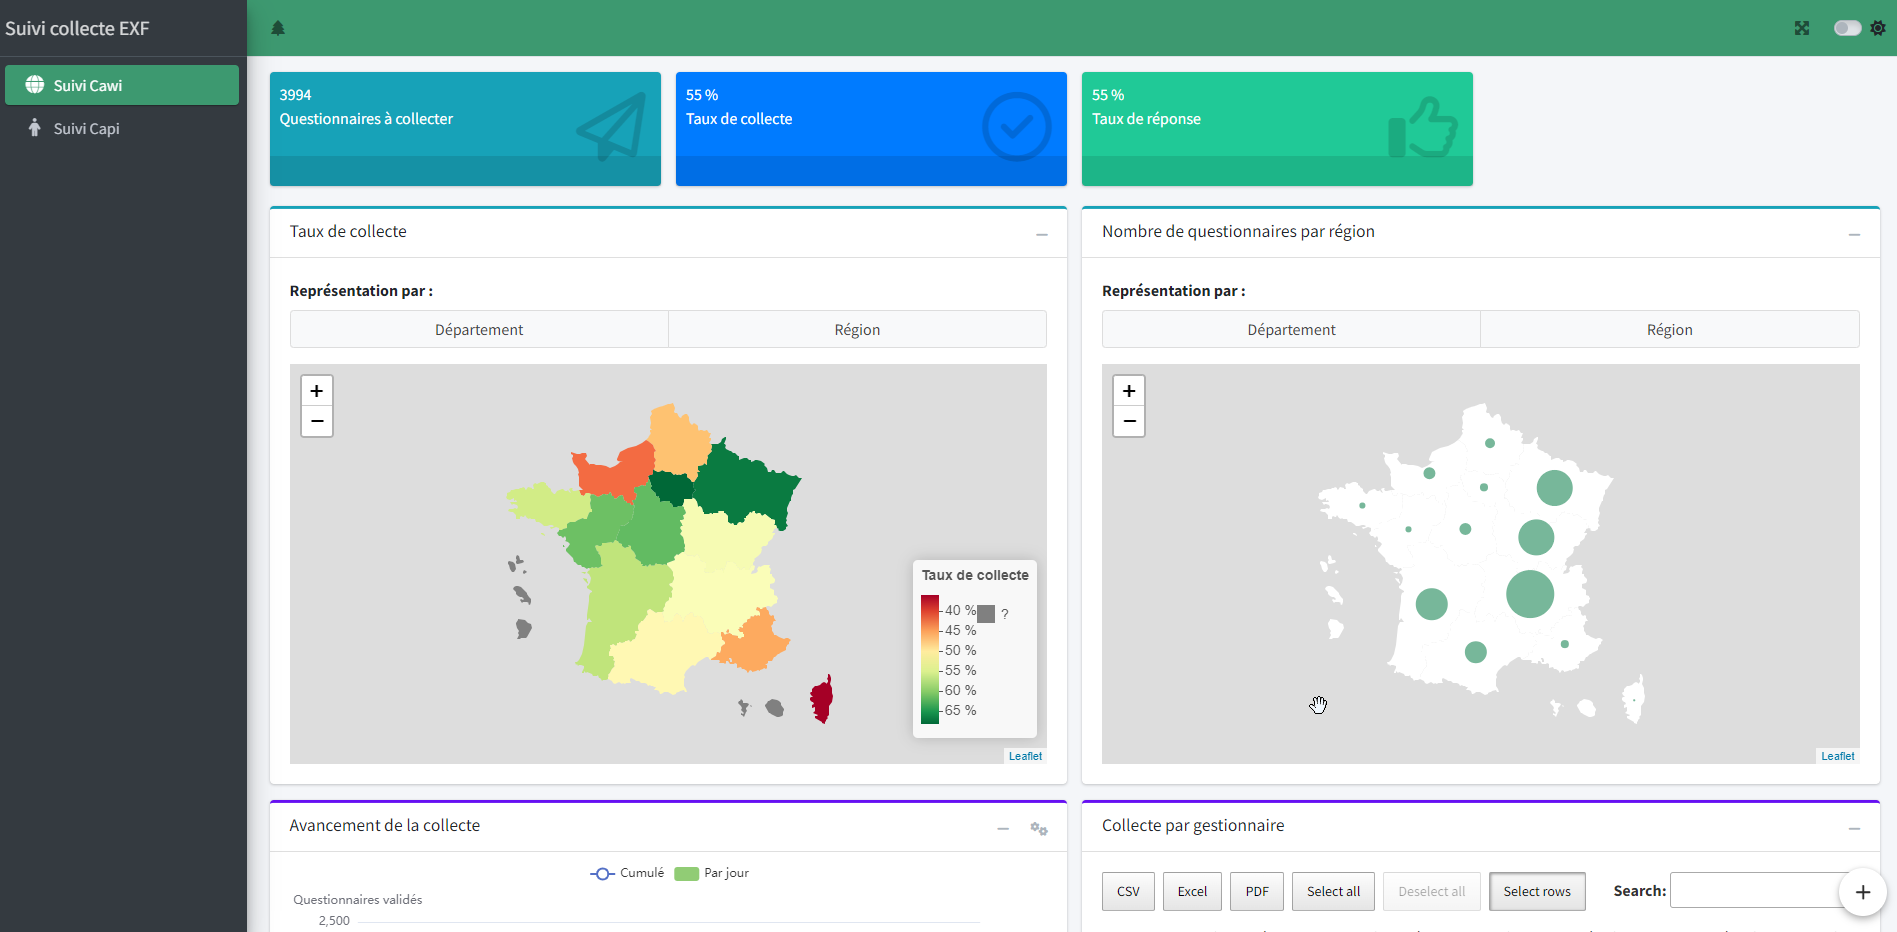
\includegraphics{./images/accueil_exf.png}

\begin{tcolorbox}[enhanced jigsaw, toprule=.15mm, rightrule=.15mm, colbacktitle=quarto-callout-warning-color!10!white, colback=white, bottomtitle=1mm, opacitybacktitle=0.6, coltitle=black, titlerule=0mm, breakable, title=\textcolor{quarto-callout-warning-color}{\faExclamationTriangle}\hspace{0.5em}{Garantie de service}, opacityback=0, toptitle=1mm, arc=.35mm, colframe=quarto-callout-warning-color-frame, leftrule=.75mm, bottomrule=.15mm, left=2mm]
La solution de suivi de collecte est basée sur un hébergement dans le
Datalab SSP Cloud. Veuillez noter qu'il n'y a aucune garantie de service
associée à cette solution. Son utilisation est basée sur la
disponibilité et les ressources actuelles, et il se peut que le service
ne soit pas toujours accessible.
\end{tcolorbox}

\bookmarksetup{startatroot}

\hypertarget{introduction}{%
\chapter{Introduction}\label{introduction}}

Les sites de suivi de collecte sont des applications internet qui
s'appuient sur les fichiers d'export de capibara pour fournir des
services utiles aux acteurs de la collecte : suivi d'avancement,
statistiques de collecte, export de listes\ldots{}

Le principe général d'architecture est assez simple :

\begin{itemize}
\tightlist
\item
  le cœur du dispositif est une application shiny, avec des packages
  additionnels pour la rendre plus efficace (bs4dash, shinywidgets,
  shinymanager\ldots),\\
\item
  cette application s'appuie sur les données exportées périodiquement
  par l'équipe SSP en charge de la collece,\\
\item
  l'application est packagée pour être déployée sur les serveurs du
  \href{https://datalab.sspcloud.fr/}{datalab SSP Cloud}.
\end{itemize}

En suivant les étapes décrites dans cette documentation, toute équipe de
collecte est capable de déployer un site de suivi.

\bookmarksetup{startatroot}

\hypertarget{pruxe9requis}{%
\chapter{Prérequis}\label{pruxe9requis}}

La création d'un site de suivi de collecte nécessite l'utilisation de
différents services gratuits. Chacun de ces services nécessite la
création d'un compte.

\hypertarget{github}{%
\section{Github}\label{github}}

(Github){[}https://github.com/{]} est un service web de stocker des
programmes informatiques et de gérer les versions de ces programmes. Les
fonctionnalités de Github qui nous intéresse pour la création des sites
de suivi de collecte :

\begin{itemize}
\tightlist
\item
  Gestion de versions : GitHub utilise Git pour permettre le suivi des
  modifications apportées aux fichiers. Vous pouvez cloner, pousser et
  tirer des référentiels Git, ce qui facilite la collaboration sur le
  code source.\\
\item
  Collaboration : GitHub permet à plusieurs contributeurs de travailler
  ensemble sur un même projet.\\
\item
  Actions GitHub; GitHub permet d'automatiser des flux de travail
  (workflows) permettant des déploiements d'application par exemple.
\end{itemize}

Pour créer un compte GitHub, suivez ces étapes :

\begin{itemize}
\tightlist
\item
  Accédez au site web de GitHub : \href{https://github.com/}{Github}
\item
  Sur la page d'accueil, vous verrez un formulaire d'inscription ``Sign
  up for Github''. Saisissez votre adresse mail pro et laissez vous
  guider.\\
\item
  Vous recevrez un e-mail de vérification à l'adresse e-mail que vous
  avez fournie. Suivez les instructions de l'e-mail pour vérifier votre
  compte.
\end{itemize}

\hypertarget{datalab-ssp-cloud}{%
\section{Datalab SSP Cloud}\label{datalab-ssp-cloud}}

Le Datalab SSP Cloud est une plateforme libre service mutualisée de
traitement de données, destinée aux statisticiens et data scientists de
l'État.

Vous pouvez vous créer un compte en allant sur la page
\href{https://datalab.sspcloud.fr/}{Datalab}, puis en haut à droit
\emph{Connexion} et \emph{Créer un compte}.

Il peut être utile de lire cette page de la documenation du datalab :
\href{https://docs.sspcloud.fr/onyxia-guide/premiere-utilisation}{Première
utilisation}

\begin{tcolorbox}[enhanced jigsaw, toprule=.15mm, rightrule=.15mm, colbacktitle=quarto-callout-tip-color!10!white, colback=white, bottomtitle=1mm, opacitybacktitle=0.6, coltitle=black, titlerule=0mm, breakable, title=\textcolor{quarto-callout-tip-color}{\faLightbulb}\hspace{0.5em}{Droits pour déposer les données}, opacityback=0, toptitle=1mm, arc=.35mm, colframe=quarto-callout-tip-color-frame, leftrule=.75mm, bottomrule=.15mm, left=2mm]
Quand votre compte est créé, contactez François Semecurbe ou Anaël
Delorme pour vous donner les droits de déposer les données.
\end{tcolorbox}

\hypertarget{jeton-daccuxe8s-personnel-github-dans-le-datalab}{%
\section{Jeton d'accès personnel Github dans le
datalab}\label{jeton-daccuxe8s-personnel-github-dans-le-datalab}}

Les programmes sont stockés sur Github et l'outil préconisé pour les
modifier est le datalab. Pour faire le lien entre les 2 outils nous
préconisons la création d'un jeton d'accès personnel côté Github, jeton
qui sera inséré dans le datalab.

\hypertarget{cruxe9ation-dun-jeton-daccuxe8s-github}{%
\subsection{Création d'un jeton d'accès
Github}\label{cruxe9ation-dun-jeton-daccuxe8s-github}}

La création d'un jeton d'accès Github est documentée par Github (en
français !) :
\href{https://docs.github.com/fr/authentication/keeping-your-account-and-data-secure/managing-your-personal-access-tokens\#cr\%C3\%A9ation-dun-personal-access-token-classic}{Création
d'un personnal access token (classic)}

\hypertarget{ajout-dans-le-datalab}{%
\subsection{Ajout dans le datalab}\label{ajout-dans-le-datalab}}

Il faut aller dans \href{https://datalab.sspcloud.fr/account}{Mon
compte} du datalab :

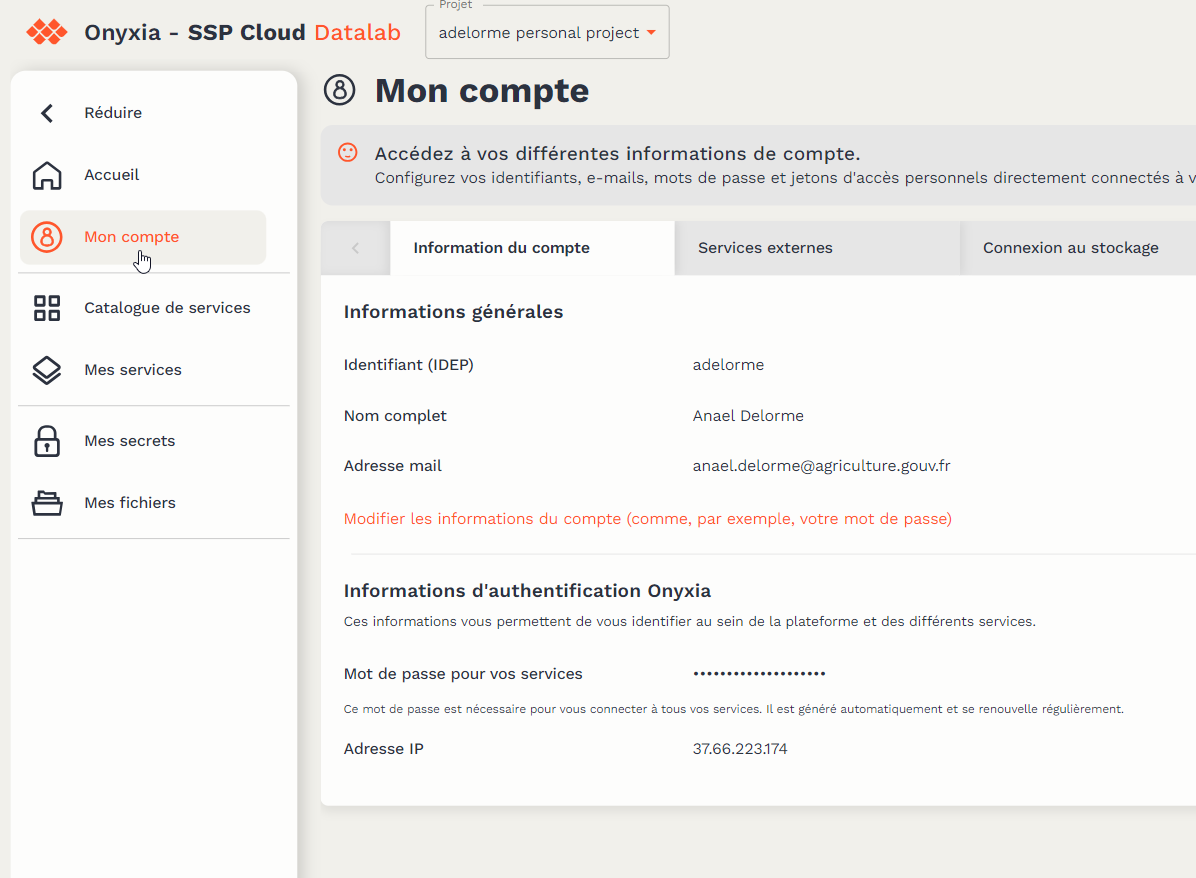
\includegraphics{./images/datalab_mon_compte.png}

Puis choisir
\href{https://datalab.sspcloud.fr/account/third-party-integration}{Service
externe} et là ajouter votre jeton Github :

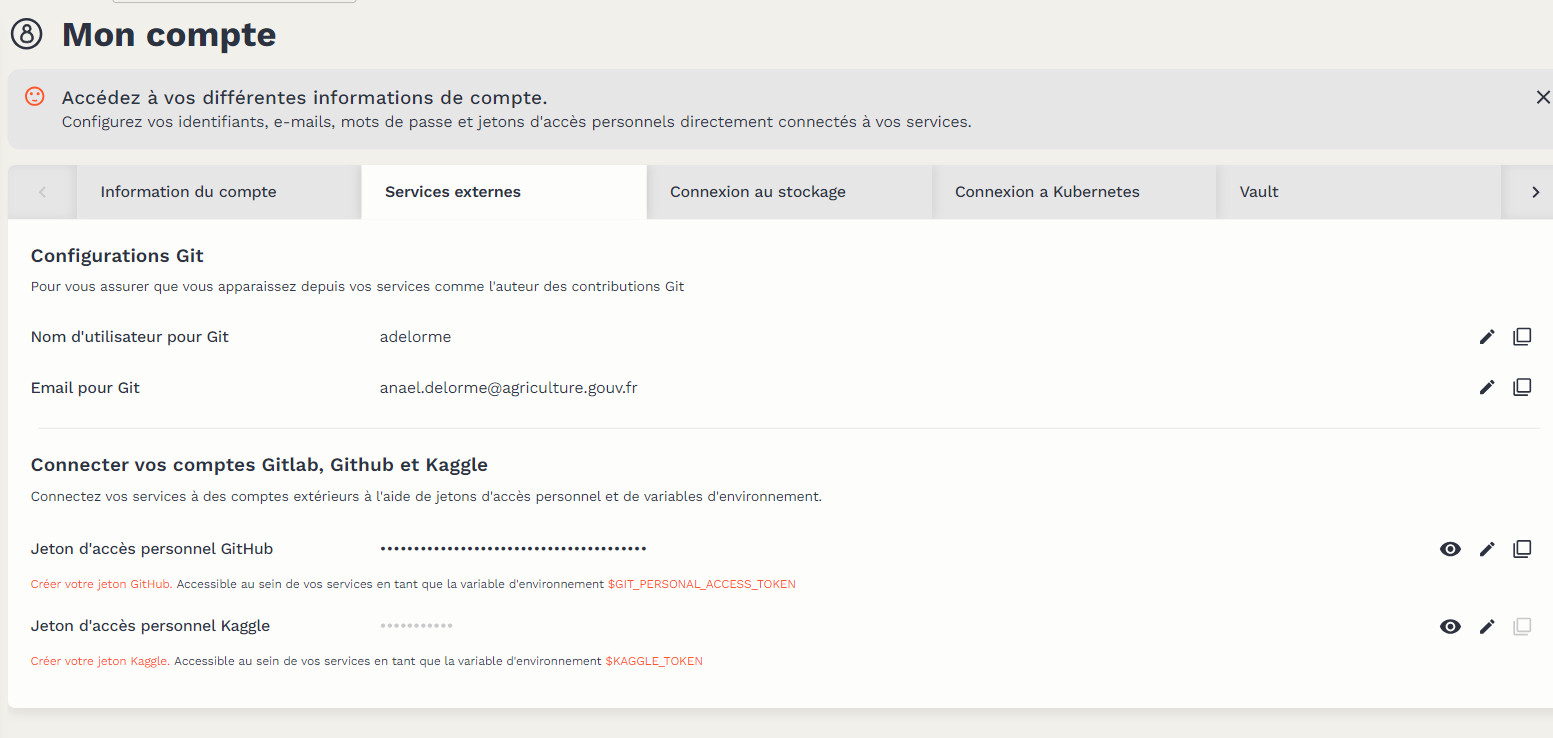
\includegraphics{./images/datalab_jeton_perso.png}

\hypertarget{dockerhub}{%
\section{DockerHub}\label{dockerhub}}

Pour déployer l'application, on a mettre l'application shiny dans un
Docker : c'est une technologie qui permet d'emballer une application ou
un logiciel, ainsi que toutes ses dépendances, dans un conteneur
virtuel. Cela permet d'assurer que l'application fonctionne de manière
fiable et de manière cohérente, quel que soit l'endroit où elle est
exécutée, que ce soit sur votre propre ordinateur, dans un centre de
données ou dans le cloud.

Le docker avec l'application shiny et ses dépendances sera stocké dans
le DockerHub : c'est une plateforme de distribution de conteneurs qui
permet aux développeurs de stocker, gérer et partager des images de
conteneurs Docker.

Pour créer un compte sur Docker Hub, suivez ces étapes :

\begin{itemize}
\tightlist
\item
  Accédez au site web de Docker Hub : \url{https://hub.docker.com}.\\
\item
  Cliquez sur le bouton ``Sign Up'' ou ``Don't have an account? Sign
  up'' pour créer un compte.\\
\item
  Suivez les étapes.\\
\item
  Vous recevrez un e-mail de vérification à l'adresse e-mail que vous
  avez fournie. Suivez les instructions de l'e-mail pour vérifier votre
  compte.
\end{itemize}

\bookmarksetup{startatroot}

\hypertarget{donnuxe9es}{%
\chapter{Données}\label{donnuxe9es}}

Les données exportées de Capibara seront déposées dans l'espace de
stockage du Datalab.

\begin{tcolorbox}[enhanced jigsaw, toprule=.15mm, rightrule=.15mm, colbacktitle=quarto-callout-important-color!10!white, colback=white, bottomtitle=1mm, opacitybacktitle=0.6, coltitle=black, titlerule=0mm, breakable, title=\textcolor{quarto-callout-important-color}{\faExclamation}\hspace{0.5em}{Utilisation de données non sensibles}, opacityback=0, toptitle=1mm, arc=.35mm, colframe=quarto-callout-important-color-frame, leftrule=.75mm, bottomrule=.15mm, left=2mm]
``Conformément aux \href{https://www.sspcloud.fr/tos_fr.md}{conditions
d'utilisation}, seules des données de type open data ou ne présentant
aucune sensibilité peuvent être stockées sur le Datalab. Le fait qu'un
fichier ait un statut de diffusion''privé'' ne suffit pas à garantir une
parfaite confidentialité.''
\end{tcolorbox}

Les données devront donc être préparées avant d'être déposées sur le
datalab.

\hypertarget{pruxe9paration-des-donnuxe9es}{%
\section{Préparation des données}\label{pruxe9paration-des-donnuxe9es}}

Toutes données permettant d'identifier une entreprise ou une personne
seront supprimées avant de remonter les données. Le format préconisé est
le parquet. Voici un exemple de code :

\begin{Shaded}
\begin{Highlighting}[]
\FunctionTok{library}\NormalTok{(tidyverse)}
\FunctionTok{library}\NormalTok{(arrow)}

\NormalTok{dossier }\OtherTok{\textless{}{-}} \FunctionTok{read.csv2}\NormalTok{(}\StringTok{"dossier.csv"}\NormalTok{)}
\NormalTok{annee\_courante }\OtherTok{\textless{}{-}} \FunctionTok{read.csv2}\NormalTok{(}\StringTok{"annee\_courante.csv"}\NormalTok{)}
\NormalTok{entreprise }\OtherTok{\textless{}{-}} \FunctionTok{read.csv2}\NormalTok{(}\StringTok{"entreprise.csv"}\NormalTok{)}
\NormalTok{gestion }\OtherTok{\textless{}{-}} \FunctionTok{read.csv2}\NormalTok{(}\StringTok{"gestion.csv"}\NormalTok{)}

\FunctionTok{write\_parquet}\NormalTok{(}\AttributeTok{x =}\NormalTok{ dossier, }\AttributeTok{sink =} \StringTok{"dossier.parquet"}\NormalTok{)}

\NormalTok{annee\_courante\_light }\OtherTok{\textless{}{-}}\NormalTok{ annee\_courante }\SpecialCharTok{\%\textgreater{}\%}
  \FunctionTok{select}\NormalTok{(Identifiant\_dossier, NOM\_DOSSIER, MAJC)}

\FunctionTok{write\_parquet}\NormalTok{(}\AttributeTok{x =}\NormalTok{ annee\_courante\_light, }\AttributeTok{sink =} \StringTok{".parquet"}\NormalTok{)}

\NormalTok{entreprise\_light }\OtherTok{\textless{}{-}}\NormalTok{ entreprise }\SpecialCharTok{\%\textgreater{}\%}
  \FunctionTok{select}\NormalTok{(}
\NormalTok{    Identifiant\_dossier,}
\NormalTok{    NOM\_DOSSIER,}
\NormalTok{    HEX\_CODE\_POSTAL\_AFFI,}
\NormalTok{    HEX\_DEPSIEGE\_AFFI,}
\NormalTok{    HEX\_REGSIEGE\_AFFI}
\NormalTok{  )}

\FunctionTok{write\_parquet}\NormalTok{(}\AttributeTok{x =}\NormalTok{ entreprise\_light, }\AttributeTok{sink =} \StringTok{"entreprise.parquet"}\NormalTok{)}

\NormalTok{gestion }\OtherTok{\textless{}{-}}\NormalTok{ gestion }\SpecialCharTok{\%\textgreater{}\%}
  \FunctionTok{select}\NormalTok{(Identifiant\_dossier, }
\NormalTok{         NOM\_DOSSIER, }
\NormalTok{         ACCEPT)}

\FunctionTok{write\_parquet}\NormalTok{(}\AttributeTok{x =}\NormalTok{ gestion, }\AttributeTok{sink =} \StringTok{"gestion.parquet"}\NormalTok{)}
\end{Highlighting}
\end{Shaded}

\hypertarget{duxe9puxf4ts-des-donnuxe9es-sur-le-datalab}{%
\section{Dépôts des données sur le
datalab}\label{duxe9puxf4ts-des-donnuxe9es-sur-le-datalab}}

Quand les données sont prépararées, il faut les déposer sur le datalab.
Le datalab offre une fonctionnalité de stockage des données (s3). Pour y
accéder, il faut aller sur le
\href{https://datalab.sspcloud.fr/}{datalab} :

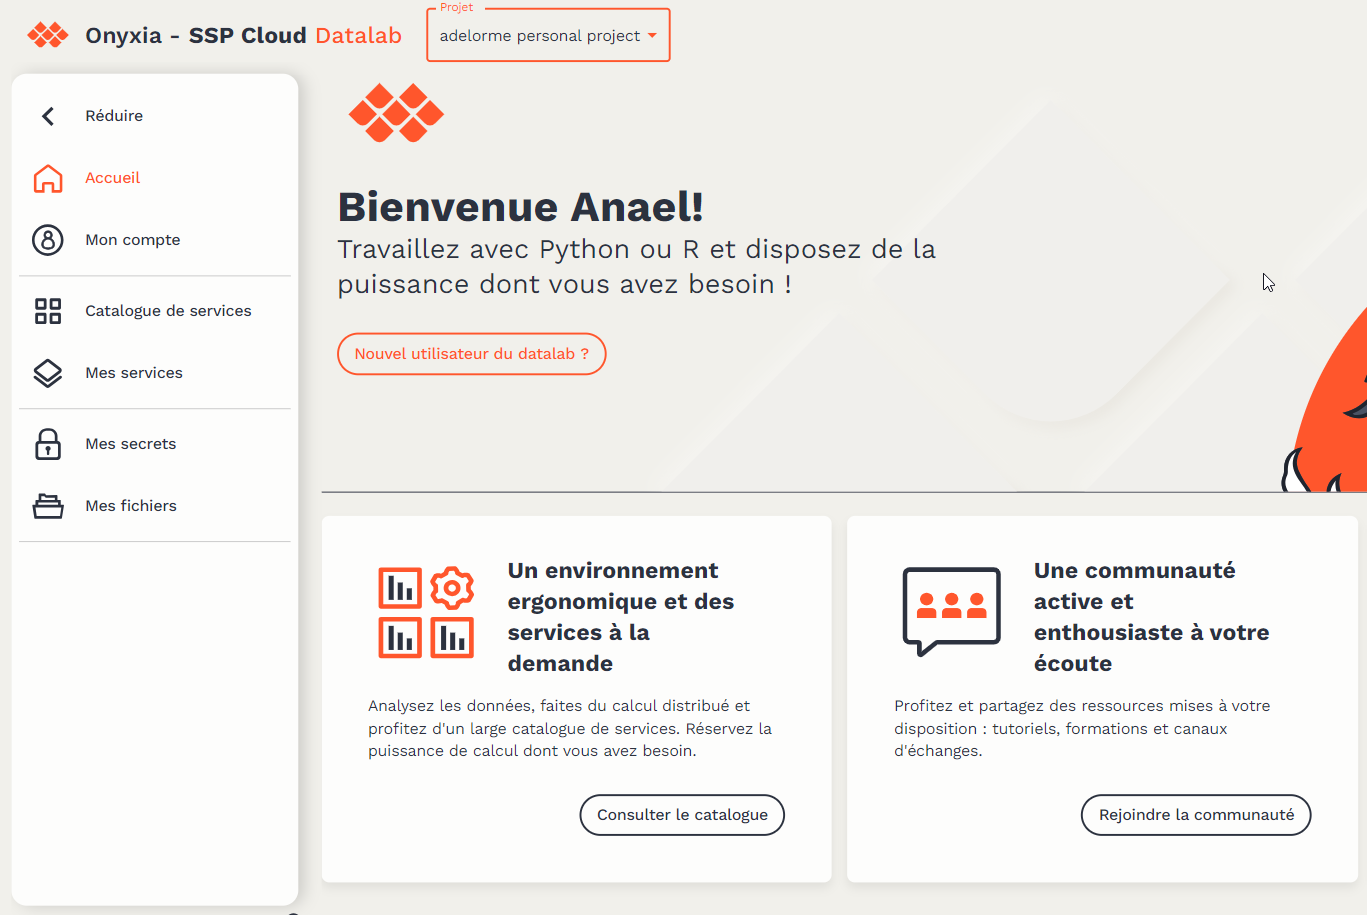
\includegraphics{./images/data_accueil_datalab.png}

Puis on choisit \emph{Mes fichiers} dans le menu de gauche :

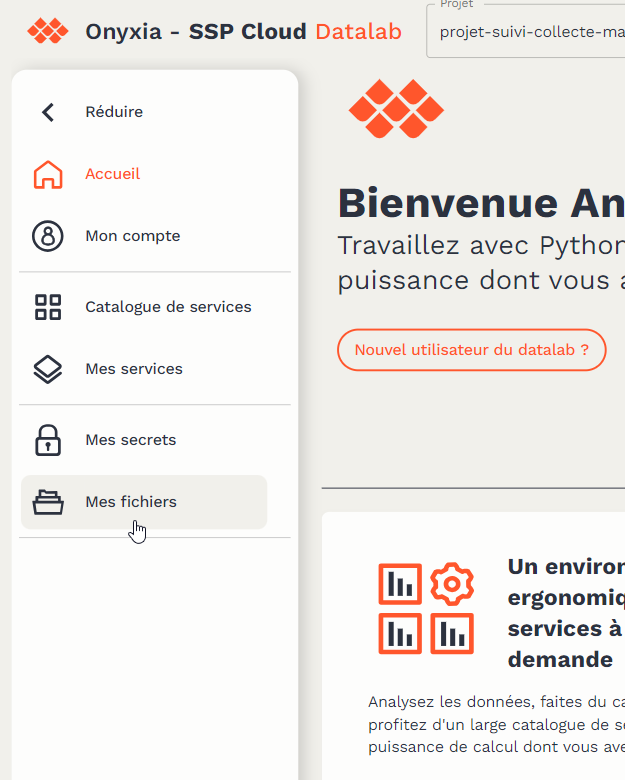
\includegraphics{./images/data_clic_mes_fichiers.png}

Là on arrive par défaut sur son lieu de stockage individuel. Pour le
site de suivi de la collecte, nous proposons d'utiliser un répertoire
(un \emph{bucket} en langage s3) partagé. Pour cela il faut choisir en
haut le projet \emph{projet\_suivi\_collecte\_masa} :

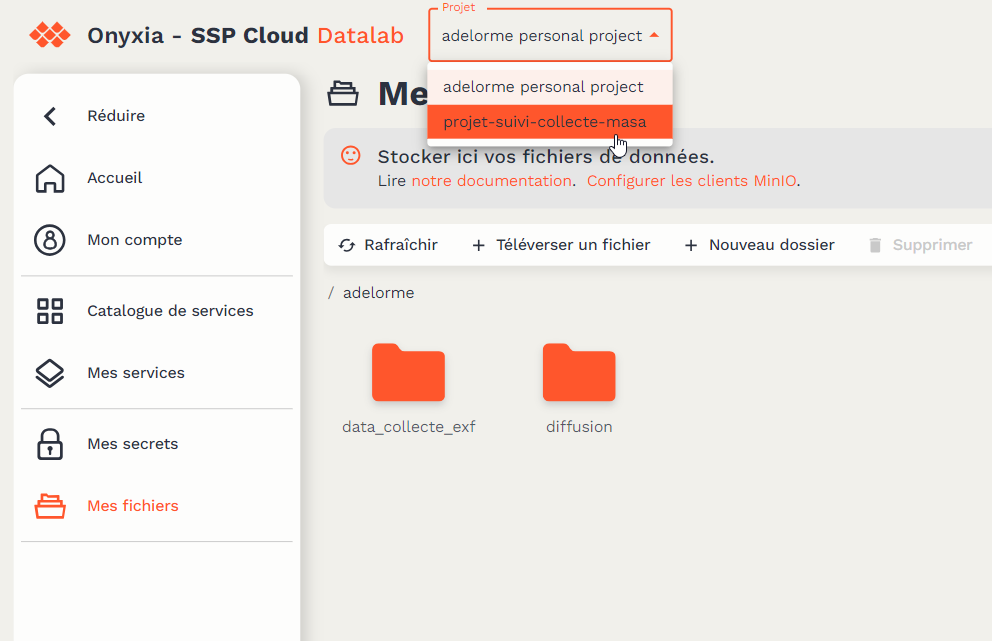
\includegraphics{./images/data_choix_projet.png}

Il ne reste plus qu'à créer un répertoire pour son site de collecte :

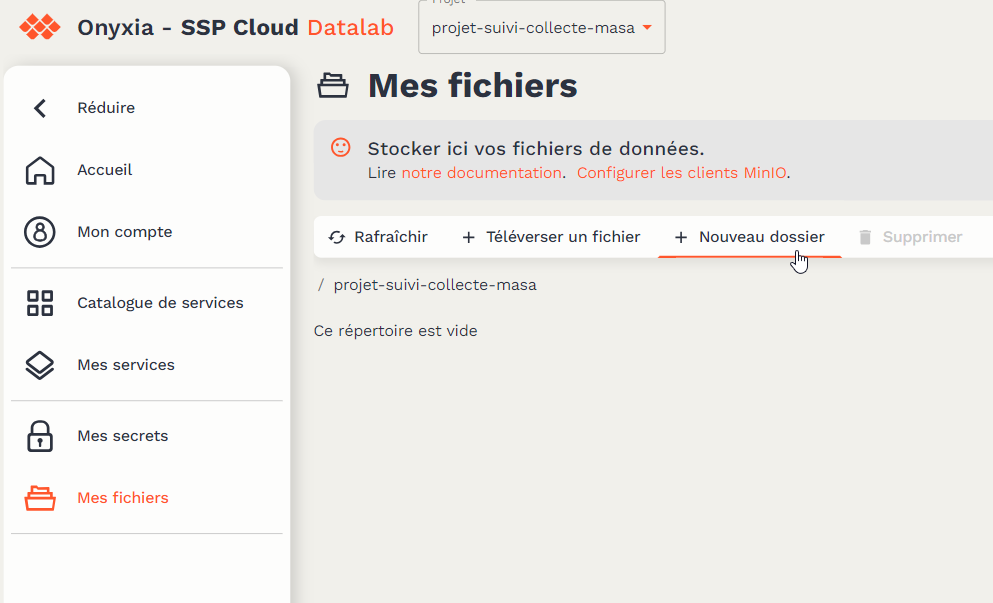
\includegraphics{./images/data_creation_nouveau_dossier.png}

En allant dans ce répertoire, il suffit de déposer le(s) fichier(s)
parquet par glisser/déposer :

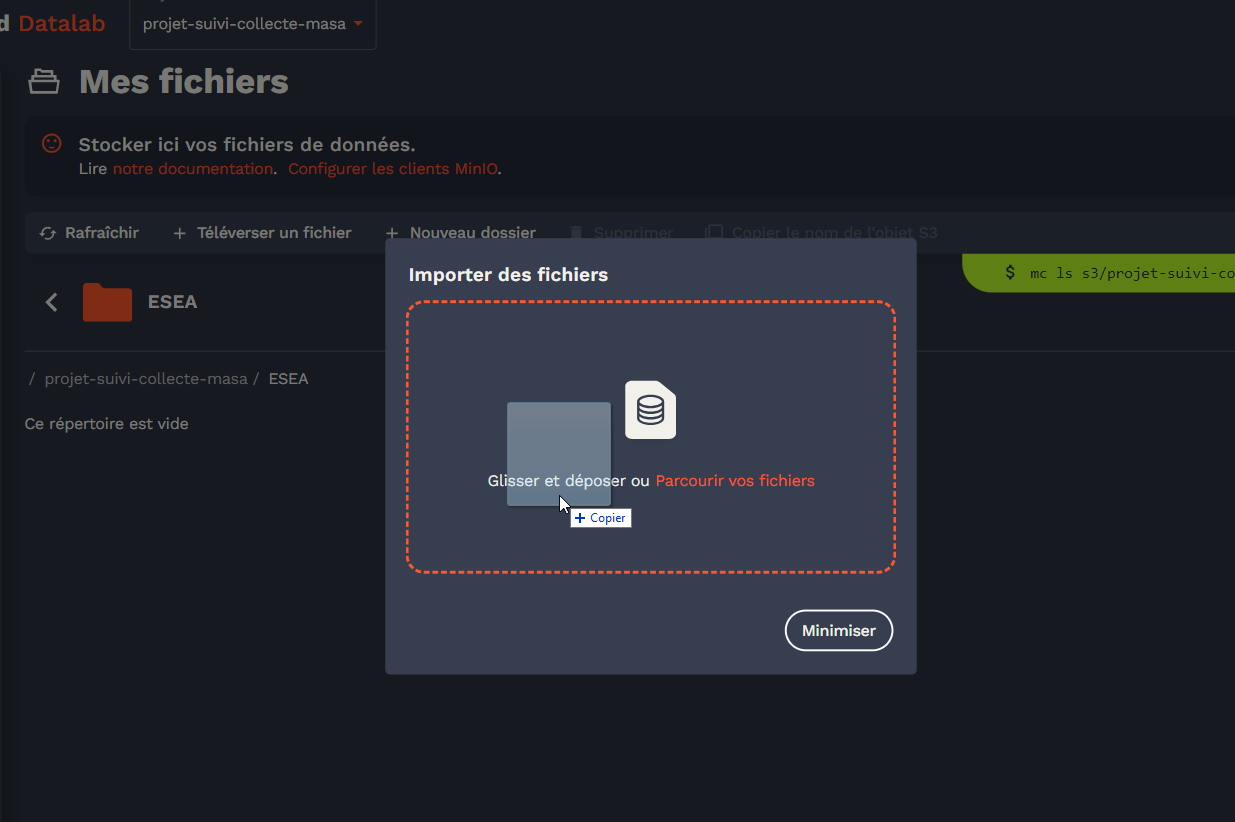
\includegraphics{./images/data_upload_data.png}

\begin{tcolorbox}[enhanced jigsaw, toprule=.15mm, rightrule=.15mm, colbacktitle=quarto-callout-tip-color!10!white, colback=white, bottomtitle=1mm, opacitybacktitle=0.6, coltitle=black, titlerule=0mm, breakable, title=\textcolor{quarto-callout-tip-color}{\faLightbulb}\hspace{0.5em}{Mise à jour des données}, opacityback=0, toptitle=1mm, arc=.35mm, colframe=quarto-callout-tip-color-frame, leftrule=.75mm, bottomrule=.15mm, left=2mm]
Régulièrement (tous les jours, toutes les semaines ?), le responsable
d'enquête mettra à jour les données. Pour cela il refera les mêmes
étapes que précédemment : export de capibara, préparation des données,
export au format parquet, téléversement dans le bucket partagé du
datalab.
\end{tcolorbox}

\bookmarksetup{startatroot}

\hypertarget{duxe9veloppement-application-shiny}{%
\chapter{Développement application
shiny}\label{duxe9veloppement-application-shiny}}

L'application de suivi de collecte est une application shiny que nous
allons déployer dans le datalab.

Pour cela nous préconisons quelques principes :

\begin{itemize}
\tightlist
\item
  utiliser le package \href{https://github.com/ThinkR-open/golem}{Golem}
  développé par Thinkr. Il encapsule l'application shiny dans un package
  avec un objectif de mise en production (inclusion de tout ce qui est
  utile au déploiement).\\
\item
  utiliser le datalab pour développer l'application.\\
\item
  stocker les programmes dans GitHub.
\end{itemize}

Cette partie de la documentation explique la mise en place de tout ce
qu'il faut pour développer l'application. Dans les prochaines parties
nous développerons le squelette du site de suivi, puis nous le
peuplerons avec des box.

\hypertarget{cruxe9ation-dun-repo-github}{%
\section{Création d'un repo Github}\label{cruxe9ation-dun-repo-github}}

Ce repo est le lieu de stockage des programmes du site de suivi de
collecte. La création de repo est réalisé par l'un des membres de
l'équipe avec son compte github (voir
\protect\hyperlink{pruxe9requis}{Prérequis}) :

\begin{itemize}
\tightlist
\item
  Se connecter à \href{https://github.com/}{Github}
\item
  Créer un nouveau repository
\end{itemize}

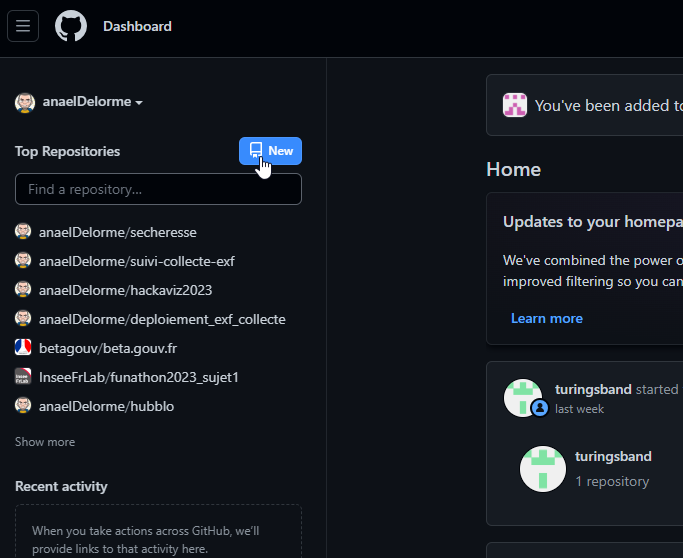
\includegraphics{./images/github_new_repository.png}

\begin{itemize}
\tightlist
\item
  saisir le nom du repo
\end{itemize}

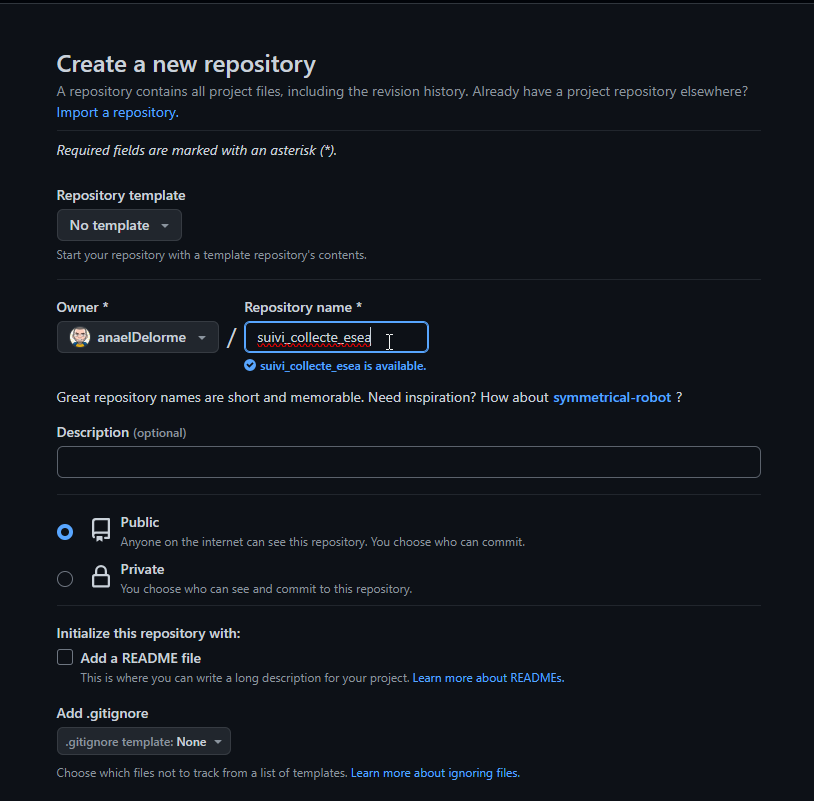
\includegraphics{./images/github_name_repository.png}

\begin{itemize}
\tightlist
\item
  laisser tout le reste tel que proposé et cliquer sur \textbf{Create
  repository}
\end{itemize}

Vous arrivez sur la page d'accueil du repo. Vous pouvez ici ajouter vos
collègues dans la rubrique \textbf{Add collaborators to this
repository}.

Avant de passer à la création du service Rstudio dans le datalab, copier
l'adresse du repo qui est disponible dans le Quick setup : dans
l'exemple ce sera
\emph{https://github.com/anaelDelorme/suivi\_collecte\_esea.git}
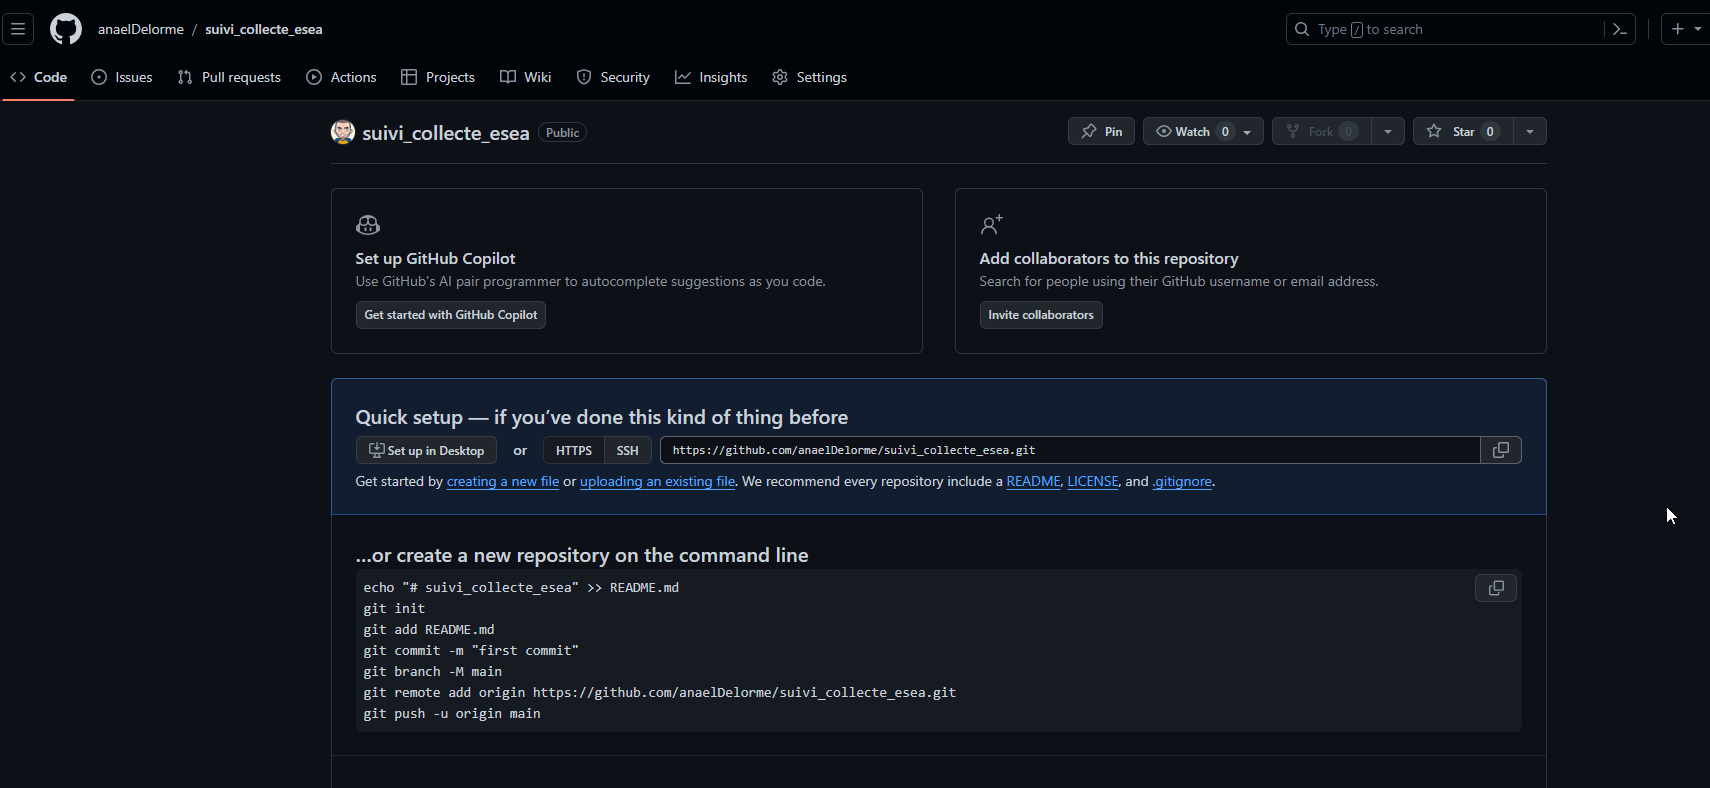
\includegraphics{./images/github_copy_link.png}

\hypertarget{cruxe9ation-dun-service-rstudio-dans-le-datalab}{%
\section{Création d'un service Rstudio dans le
datalab}\label{cruxe9ation-dun-service-rstudio-dans-le-datalab}}

Vous pourriez tout à fait travailler sur Cerise ou sur votre poste
local. Nous vous proposons de travailler sur le datalab directement :
vous avez accès à une configuration proche de celle du déploiement de
votre site. Et nous vous conseillons d'utiliser un VSCode plutôt qu'un
Rstudio.

Après vous être connecté au datalab, vous aller dans \emph{Mes
services}.

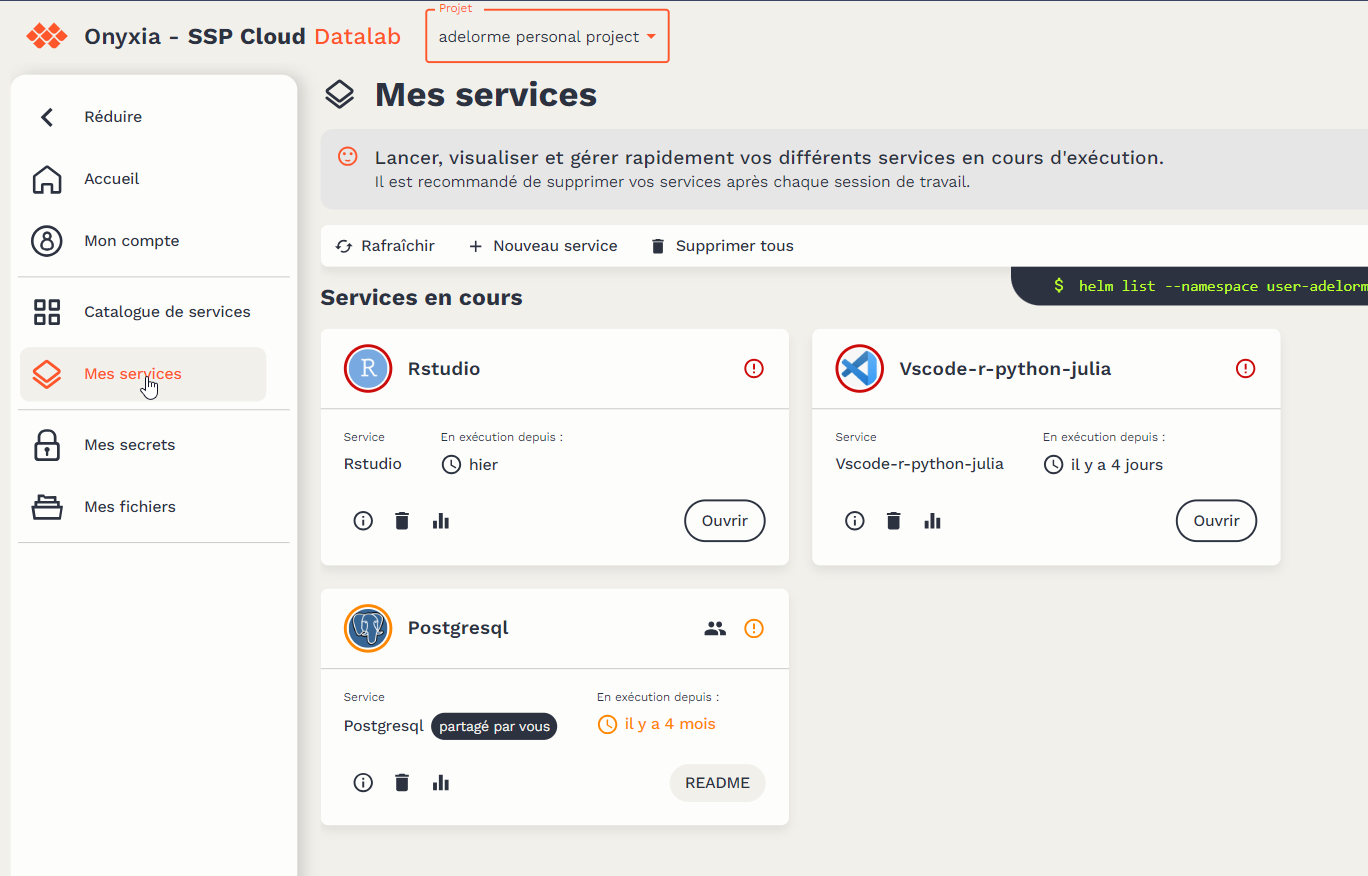
\includegraphics{./images/datalab_mes_services.png}

Puis vous cliquer sur \emph{Nouveau service} :

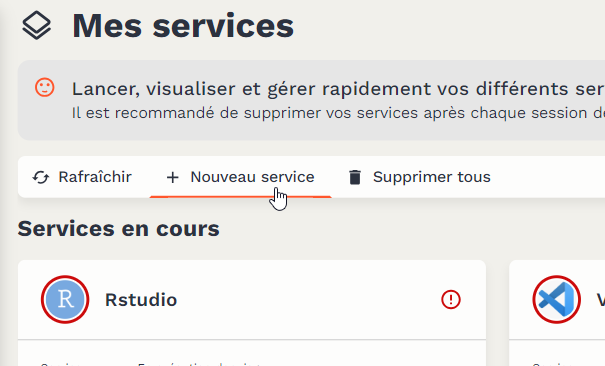
\includegraphics{./images/datalab_nouveau_service.png}

Vous choisissez un Vscode-r-python-julia. Là nous utiliserons Rstudio en
cliquant sur Lancer :

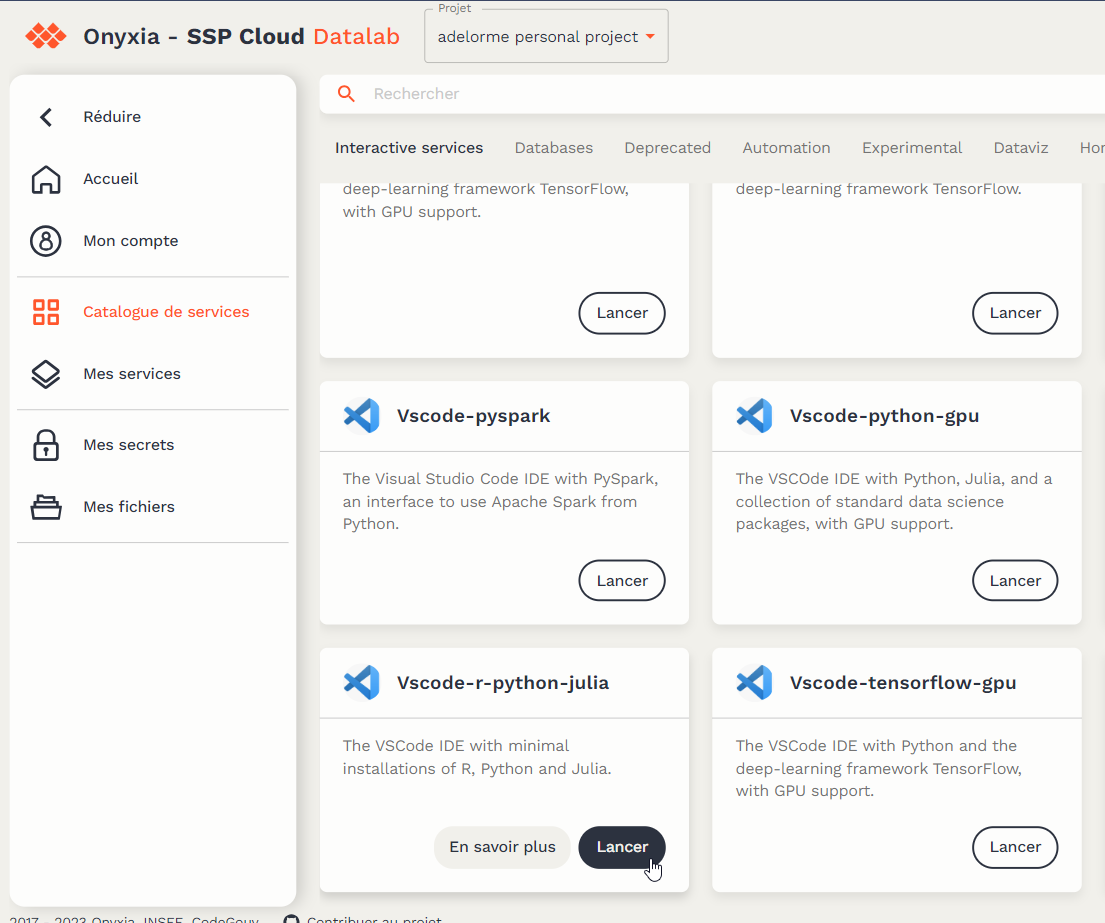
\includegraphics{./images/datalab_vscode_service.png}

Avant de lancer le service nous conseillons de le configurer en ouvrant
la boite \emph{Configuration Vscode}, puis d'aller dans l'onglet
\emph{Git}. Il faut recopier dans Repository le lien du repo copié
précédemment et vérifier les identifiants et token github :

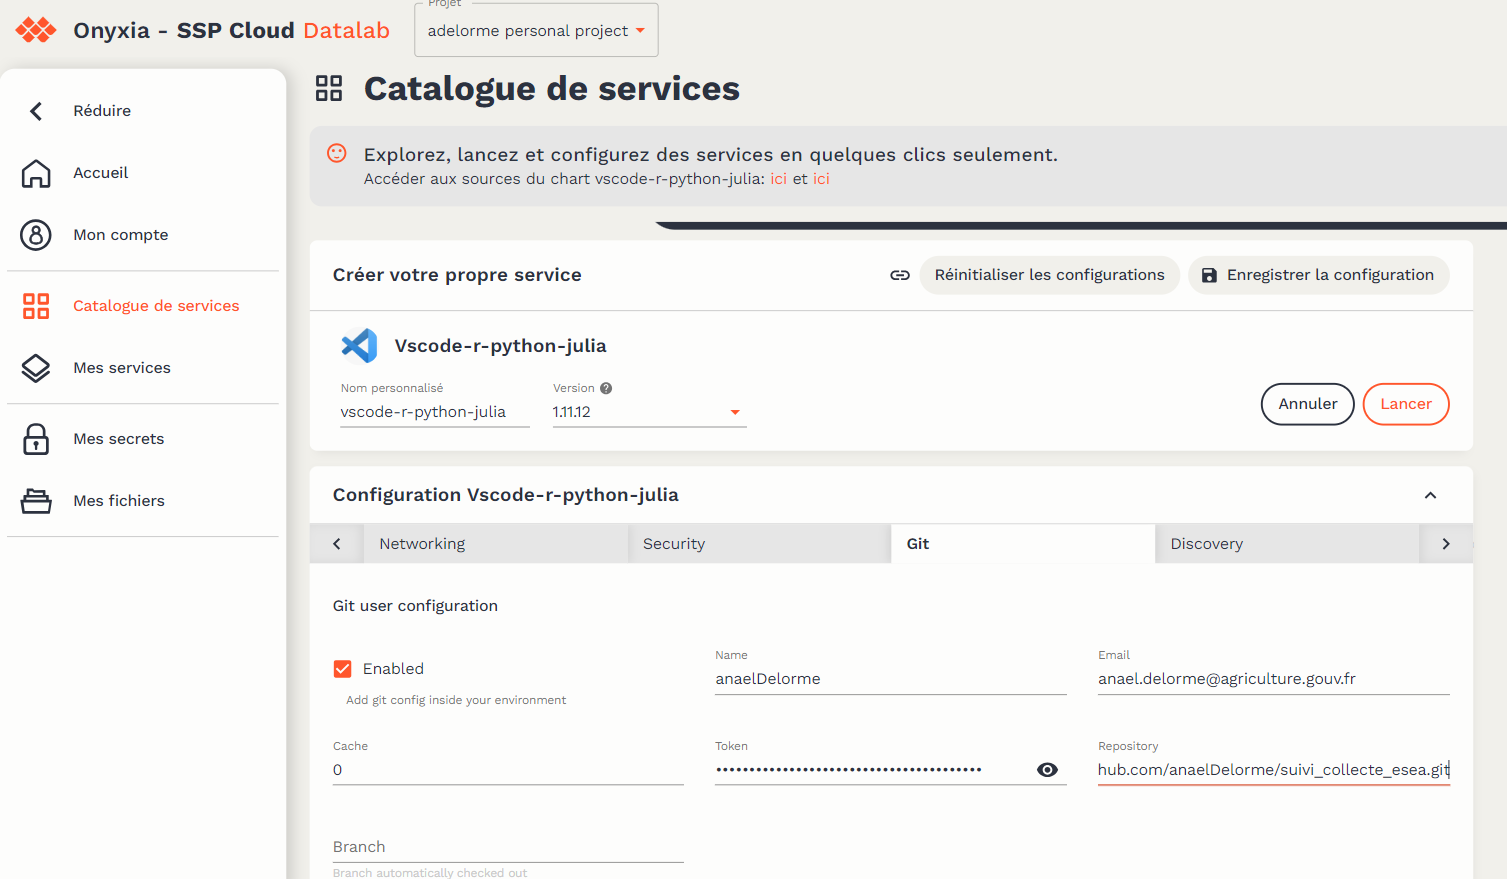
\includegraphics{./images/conf_git_vscode.png}

Puis clikquer sur \emph{Lancer}. Après quelques instants le service
Vscode sera disponible et vous pourrez vous y connectant avec le mot de
passe indiqué à l'écran.

Si tout s'est bien passé, vous arrivez dans un Vscode classique avec un
répertoire vide correspondant au répertoire du Github.

\hypertarget{installation-des-packages-utiles}{%
\section{Installation des packages
utiles}\label{installation-des-packages-utiles}}

La création d'un site de suivi de collecte nécessite l'installation de
packages. Pour cela, ouvrez un terminal VScode :

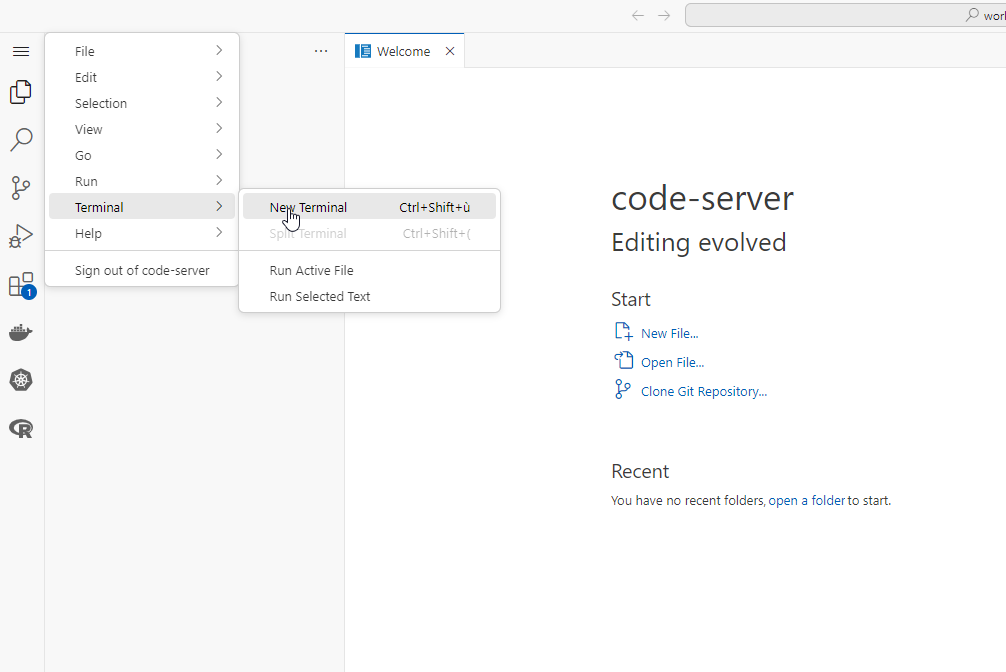
\includegraphics{./images/VSCode_new_terminal.png}

Tapez r pour indiquer que vous allez saisir une commande R. Puis lancer
la ligne de code suivante.

\begin{Shaded}
\begin{Highlighting}[]
\FunctionTok{install.packages}\NormalTok{(}\FunctionTok{c}\NormalTok{(}\StringTok{"tidyverse"}\NormalTok{, }\StringTok{"arrow"}\NormalTok{, }\StringTok{"shiny"}\NormalTok{, }\StringTok{"shinyWidgets"}\NormalTok{, }\StringTok{"bs4Dash"}\NormalTok{, }\StringTok{"shinymanager"}\NormalTok{, }\StringTok{"leaflet"}\NormalTok{, }\StringTok{"config"}\NormalTok{, }\StringTok{"DT"}\NormalTok{, }\StringTok{"echarts4r"}\NormalTok{, }\StringTok{"geojsonio"}\NormalTok{, }\StringTok{"glue"}\NormalTok{, }\StringTok{"golem"}\NormalTok{, }\StringTok{"htmlwidgets"}\NormalTok{, }\StringTok{"janitor"}\NormalTok{, }\StringTok{"sf"}\NormalTok{, }\StringTok{"testthat"}\NormalTok{, }\StringTok{"geojsonio"}\NormalTok{, }\StringTok{"dockerfiler"}\NormalTok{, }\StringTok{"attachment"}\NormalTok{, }\StringTok{"rsconnect"}\NormalTok{, }\StringTok{"spelling"}\NormalTok{, }\StringTok{"aws.s3"}\NormalTok{, }\StringTok{"waiter"}\NormalTok{, }\StringTok{"pandoc"}\NormalTok{))}
\end{Highlighting}
\end{Shaded}

\hypertarget{cruxe9ation-du-projet-golem}{%
\section{Création du projet Golem}\label{cruxe9ation-du-projet-golem}}

Allez dans le répertoire créé dans votre Rstudio, créer un répertoire
\emph{suiviCollecte}, puis créer un fichier \emph{init.R} et indiquez la
ligne de code suivante :

\begin{Shaded}
\begin{Highlighting}[]
\NormalTok{golem}\SpecialCharTok{::}\FunctionTok{create\_golem}\NormalTok{(}\AttributeTok{path =} \StringTok{"../suiviCollecte"}\NormalTok{, }\AttributeTok{check\_name =} \ConstantTok{TRUE}\NormalTok{)}
\end{Highlighting}
\end{Shaded}

Lancez la commande.

Vous obtenez un répertoire suiviCollecte dans votre répertoire
suivi\_collecte\_XXX qui sera votre répertoire de travail pour créer
votre application shiny. Si le répertoire suiviCollecte n'est pas créé
comme sous-répertoire de suivi\_collecte\_XXX, déplacer le.

\hypertarget{paramuxe9trage-golem-de-votre-package}{%
\section{Paramétrage Golem de votre
package}\label{paramuxe9trage-golem-de-votre-package}}

Le principe de Golem est d'encapsuler l'application shiny dans un
package. Il y a quelques étapes à suivre afin de commencer à développer
l'application shiny. Dans le répertoire Dev, ouvrez le fichier 01\_start
puis modifier et lancer les différentes commandes:

\begin{itemize}
\tightlist
\item
  Description du package :
\end{itemize}

\begin{Shaded}
\begin{Highlighting}[]
\NormalTok{golem}\SpecialCharTok{::}\FunctionTok{fill\_desc}\NormalTok{(}
  \AttributeTok{pkg\_name =} \StringTok{"suiviCollecte"}\NormalTok{, }\CommentTok{\# The Name of the package containing the App}
  \AttributeTok{pkg\_title =} \StringTok{"Suivi de la collecte ESEA"}\NormalTok{, }\CommentTok{\# The Title of the package containing the App}
  \AttributeTok{pkg\_description =} \StringTok{"Site web de suivi de la collecte de l\textquotesingle{}enquête ESEA"}\NormalTok{, }\CommentTok{\# The Description of the package containing the App}
  \AttributeTok{author\_first\_name =} \StringTok{"Anaël"}\NormalTok{, }\CommentTok{\# Your First Name}
  \AttributeTok{author\_last\_name =} \StringTok{"Delorme"}\NormalTok{, }\CommentTok{\# Your Last Name}
  \AttributeTok{author\_email =} \StringTok{"anael.delorme@agriculture.gouv.Fr"}\NormalTok{, }\CommentTok{\# Your Email}
  \AttributeTok{repo\_url =} \StringTok{"https://github.com/anaelDelorme/suivi\_collecte\_esea"}\NormalTok{, }\CommentTok{\# The URL of the GitHub Repo (optional),}
  \AttributeTok{pkg\_version =} \StringTok{"0.0.0.9000"} \CommentTok{\# The Version of the package containing the App}
\NormalTok{)}
\end{Highlighting}
\end{Shaded}

\begin{itemize}
\tightlist
\item
  Lancement des commandes utiles :
\end{itemize}

\begin{Shaded}
\begin{Highlighting}[]
\DocumentationTok{\#\#\#\#\#\#\#\#\#\#\#\#\#\#\#\#\#\#\#\# A LANCER}

\DocumentationTok{\#\# Set \{golem\} options {-}{-}{-}{-}}
\NormalTok{golem}\SpecialCharTok{::}\FunctionTok{set\_golem\_options}\NormalTok{()}

\DocumentationTok{\#\# Install the required dev dependencies {-}{-}{-}{-}}
\NormalTok{golem}\SpecialCharTok{::}\FunctionTok{install\_dev\_deps}\NormalTok{()}

\DocumentationTok{\#\# Create Common Files {-}{-}{-}{-}}
\DocumentationTok{\#\# See ?usethis for more information}
\NormalTok{usethis}\SpecialCharTok{::}\FunctionTok{use\_mit\_license}\NormalTok{(}\StringTok{"Golem User"}\NormalTok{) }\CommentTok{\# You can set another license here}
\NormalTok{usethis}\SpecialCharTok{::}\FunctionTok{use\_readme\_rmd}\NormalTok{(}\AttributeTok{open =} \ConstantTok{FALSE}\NormalTok{)}
\NormalTok{devtools}\SpecialCharTok{::}\FunctionTok{build\_readme}\NormalTok{()}
\CommentTok{\# Note that \textasciigrave{}contact\textasciigrave{} is required since usethis version 2.1.5}
\CommentTok{\# If your \{usethis\} version is older, you can remove that param}
\NormalTok{usethis}\SpecialCharTok{::}\FunctionTok{use\_code\_of\_conduct}\NormalTok{(}\AttributeTok{contact =} \StringTok{"Golem User"}\NormalTok{)}
\NormalTok{usethis}\SpecialCharTok{::}\FunctionTok{use\_lifecycle\_badge}\NormalTok{(}\StringTok{"Experimental"}\NormalTok{)}
\NormalTok{usethis}\SpecialCharTok{::}\FunctionTok{use\_news\_md}\NormalTok{(}\AttributeTok{open =} \ConstantTok{FALSE}\NormalTok{)}


\DocumentationTok{\#\# Init Testing Infrastructure {-}{-}{-}{-}}
\DocumentationTok{\#\# Create a template for tests}
\NormalTok{golem}\SpecialCharTok{::}\FunctionTok{use\_recommended\_tests}\NormalTok{()}

\DocumentationTok{\#\# Favicon {-}{-}{-}{-}}
\CommentTok{\# If you want to change the favicon (default is golem\textquotesingle{}s one)}
\NormalTok{golem}\SpecialCharTok{::}\FunctionTok{use\_favicon}\NormalTok{() }\CommentTok{\# path = "path/to/ico". Can be an online file.}
\CommentTok{\# golem::remove\_favicon() \# Uncomment to remove the default favicon}

\DocumentationTok{\#\# Add helper functions {-}{-}{-}{-}}
\NormalTok{golem}\SpecialCharTok{::}\FunctionTok{use\_utils\_ui}\NormalTok{(}\AttributeTok{with\_test =} \ConstantTok{TRUE}\NormalTok{)}
\NormalTok{golem}\SpecialCharTok{::}\FunctionTok{use\_utils\_server}\NormalTok{(}\AttributeTok{with\_test =} \ConstantTok{TRUE}\NormalTok{)}

\DocumentationTok{\#\#\#\#\#\#\#\#\#\#\#\#\#\#\#\#\#\# NE PAS LANCER}
\DocumentationTok{\#\# Use git {-}{-}{-}{-}}
\NormalTok{usethis}\SpecialCharTok{::}\FunctionTok{use\_git}\NormalTok{()}
\end{Highlighting}
\end{Shaded}

Dans le répertoire Dev, ouvrez le fichier 02\_start puis lancer les
différentes commandes:

\begin{Shaded}
\begin{Highlighting}[]
\DocumentationTok{\#\#\# A Lancer :}

\NormalTok{attachment}\SpecialCharTok{::}\FunctionTok{att\_amend\_desc}\NormalTok{()}

\DocumentationTok{\#\# Creates fct\_* and utils\_*}
\NormalTok{golem}\SpecialCharTok{::}\FunctionTok{add\_fct}\NormalTok{(}\StringTok{"helpers"}\NormalTok{, }\AttributeTok{with\_test =} \ConstantTok{TRUE}\NormalTok{)}
\NormalTok{golem}\SpecialCharTok{::}\FunctionTok{add\_utils}\NormalTok{(}\StringTok{"helpers"}\NormalTok{, }\AttributeTok{with\_test =} \ConstantTok{TRUE}\NormalTok{)}

\DocumentationTok{\#\# Vignette {-}{-}{-}{-}}
\NormalTok{usethis}\SpecialCharTok{::}\FunctionTok{use\_vignette}\NormalTok{(}\StringTok{"suiviCollecte"}\NormalTok{)}
\NormalTok{devtools}\SpecialCharTok{::}\FunctionTok{build\_vignettes}\NormalTok{()}


\DocumentationTok{\#\#\#\#\#\#\#\#\#\#\#\#\#\# Ne pas lancer le reste}
\end{Highlighting}
\end{Shaded}

\hypertarget{commit-et-push-dans-github}{%
\section{Commit et push dans github}\label{commit-et-push-dans-github}}

Vous êtes prêts à lancer le développement de votre application shiny.
Nous vous recommandons de faire un commit / push de votre code dans
Github. Pour cela il faut :

\begin{itemize}
\tightlist
\item
  aller dans *Source control'' :
\end{itemize}

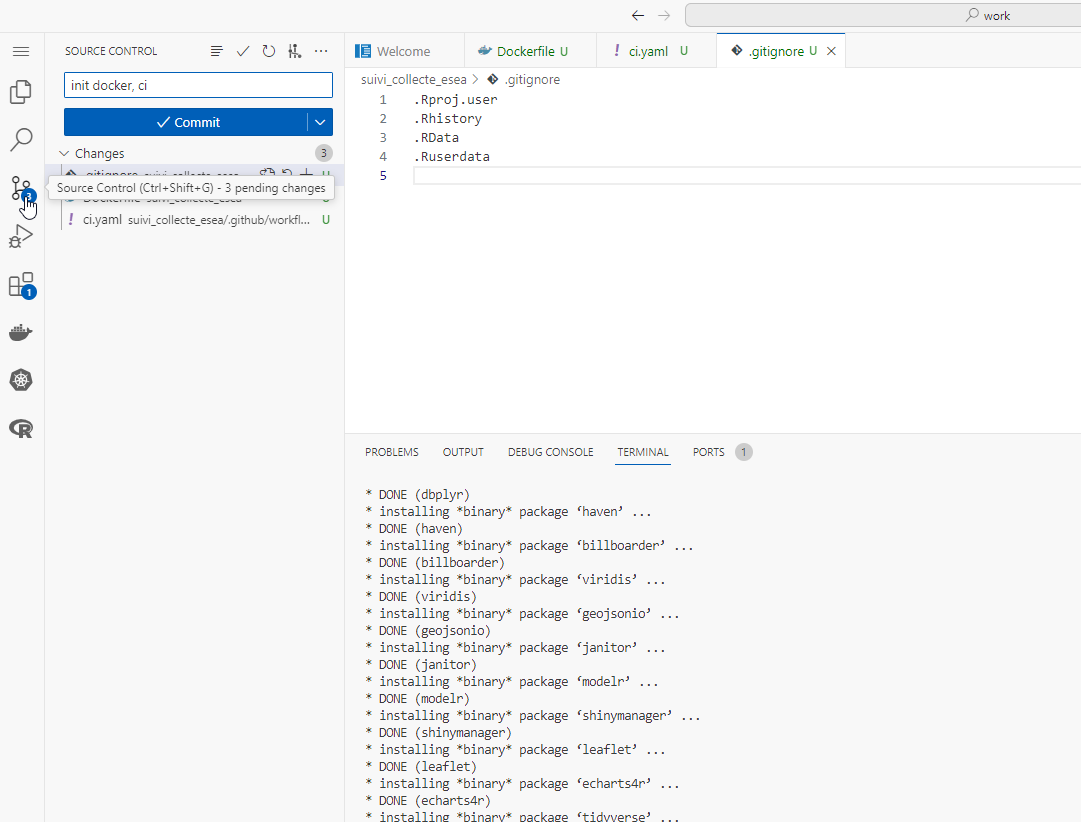
\includegraphics{./images/vscode_first_git.png}

\begin{itemize}
\tightlist
\item
  là il faut indiquer que tous les fichiers doivent être dans le commit
  et envoyés dans Github. En langague git, c'est \emph{stage all
  changes}. Dans VScode c'est le bouton + à droite de \emph{Changes}.
\end{itemize}

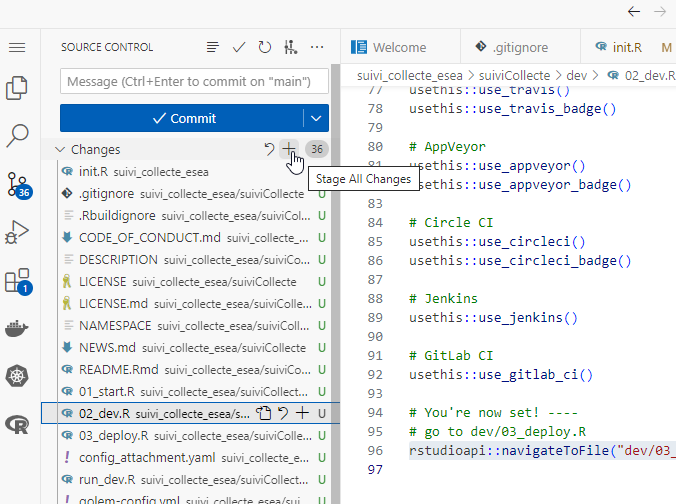
\includegraphics{./images/vscode_stade_all_changes.png}

\begin{itemize}
\tightlist
\item
  indiquer un libellé de commit puis à droite du Commit, choisir Commit
  \& Push.
\end{itemize}

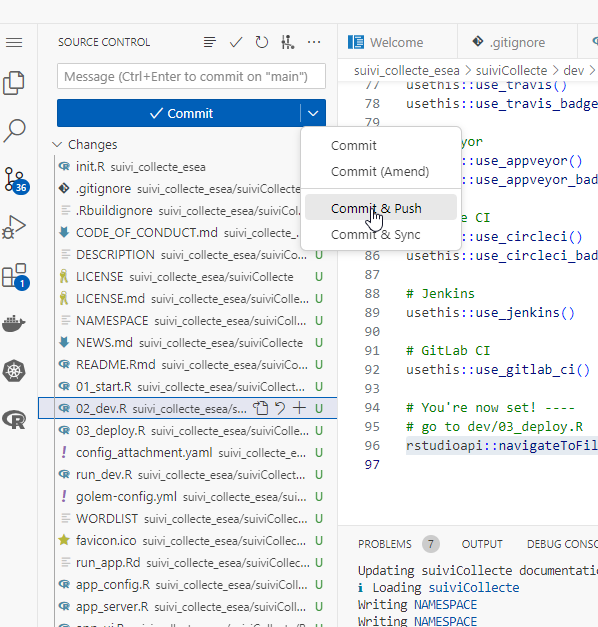
\includegraphics{./images/golem_commit_and_push.png}

\begin{itemize}
\tightlist
\item
  vérifiez dans Github que le code a bien été envoyé.
\end{itemize}

\bookmarksetup{startatroot}

\hypertarget{squelette-de-lapplication-shiny}{%
\chapter{Squelette de l'application
Shiny}\label{squelette-de-lapplication-shiny}}

L'application shiny sera propulsée par
\href{https://rinterface.github.io/bs4Dash/index.html}{bs4Dash} dans le
cadre fourni par Golem.

\hypertarget{schuxe9ma-dune-page-bs4dash}{%
\section{Schéma d'une page bs4Dash}\label{schuxe9ma-dune-page-bs4dash}}

Une page de bs4Dah contient :

\begin{itemize}
\tightlist
\item
  un menu latéral = dashboardSidebar\\
\item
  un haut de page = dashboardHeader\\
\item
  un corps de page = dashboardBody qui contient des bs4ValueBox et des
  tabBox
\end{itemize}

\includegraphics{./images/PA-bs4Dash.gif}

\hypertarget{organisation-des-programmes-avec-golem}{%
\section{Organisation des programmes avec
Golem}\label{organisation-des-programmes-avec-golem}}

En shiny il y a traditionnellement une fonction pour l'interface
utilisateur \textbf{ui} et une pour les calculs côté serveur
\textbf{server}. Ce qui permet de lancer la fonction shinyApp avec les 2
paramètres ui et server.

En Golem l'architecture est quelque peu différente avec une organisation
plus modulaire qui permet une plus grande flexibilité. Les programmes
sont dans le répertoire \textbf{R}. Suite à l'initialisation du siten il
y a plusieurs fonctions qui ont été créées. Pour notre besoin, nous
allons seulement regarder les programmes \textbf{app\_server.R} et
\textbf{app\_ui.R}. Ces programmes sont le coeur de notre site. Pour
développer notre site, nous allons créé des \textbf{modules} qui seront
utilisés par ses programmes app\_server et app\_ui

\hypertarget{app_server.r}{%
\subsection{app\_server.R}\label{app_server.r}}

Ce programme ne contient qu'une seule fonction \textbf{app\_server()}
qui est vide pour l'instant. Ici seront copiés les fonctions server de
chacun des modules que nous allons créé.

\hypertarget{app_ui.r}{%
\subsection{app\_ui.R}\label{app_ui.r}}

Cet programme contient les fonctions nécessaires à l'affichage de
l'application : app\_ui pour l'affichage global et
golem\_add\_external\_resources pour ajouter/définir des ressources
externes comme le favicon ou le titre de l'application par exemple.

C'est la fonction app\_ui qui permet de définir le squelleet de la page.
Dans le \textbf{tagList}, on va créer une dashbordPage qui contient le
sidebar, le body et un footer :

\begin{Shaded}
\begin{Highlighting}[]
\FunctionTok{library}\NormalTok{(tidyverse)}
\FunctionTok{library}\NormalTok{(arrow)}

\NormalTok{app\_ui }\OtherTok{\textless{}{-}} \ControlFlowTok{function}\NormalTok{(request) \{}
  \FunctionTok{tagList}\NormalTok{(}
    \CommentTok{\# TOUJOURS laisser cette fonction}
    \FunctionTok{golem\_add\_external\_resources}\NormalTok{(),}
    
    \CommentTok{\# Création de la page}
\NormalTok{    bs4Dash}\SpecialCharTok{::}\FunctionTok{dashboardPage}\NormalTok{(}
      \CommentTok{\# Titre général}
      \AttributeTok{title =} \StringTok{"Suivi collecte EXF"}\NormalTok{,}
      \CommentTok{\# Ajouter le bouton en haut à droite permettant d\textquotesingle{}ouvrir le site en page complète}
      \AttributeTok{fullscreen =} \ConstantTok{TRUE}\NormalTok{,}
      \CommentTok{\# Jout d\textquotesingle{}un waiter}
      \AttributeTok{preloader =} \FunctionTok{list}\NormalTok{(}\AttributeTok{html =}\NormalTok{ waiter}\SpecialCharTok{::}\FunctionTok{spin\_flower}\NormalTok{(), }\AttributeTok{color =} \StringTok{"\#6610f2"}\NormalTok{),}
      \CommentTok{\# Création du header}
      \AttributeTok{header =}\NormalTok{ bs4Dash}\SpecialCharTok{::}\FunctionTok{dashboardHeader}\NormalTok{(}
        \CommentTok{\# Titre du header qui se met en haut à gauche du site}
        \AttributeTok{title =} \StringTok{"Suivi collecte EXF"}\NormalTok{,}
        \CommentTok{\# Couleur du header {-}{-}\textgreater{} choix de couleurs dans le help de bs4Dash : ?bs4Dash::dashboardHeader}
        \AttributeTok{status =} \StringTok{"olive"}\NormalTok{,}
        \CommentTok{\# logo à gauche du header qui permet d\textquotesingle{}ouvrir et fermer le menu latéral}
        \CommentTok{\# possibilité d\textquotesingle{}utiliser les logos de bootstrap : https://fontawesome.com/icons ou https://getbootstrap.com/docs/3.3/components/\#glyphicons}
        \AttributeTok{sidebarIcon =}\NormalTok{ shiny}\SpecialCharTok{::}\FunctionTok{icon}\NormalTok{(}\StringTok{"tree"}\NormalTok{)}
\NormalTok{      ),}
      \CommentTok{\# Création du menu latéral}
      \AttributeTok{sidebar =} \FunctionTok{dashboardSidebar}\NormalTok{(}
        \CommentTok{\# Couleur du menu latéral}
        \AttributeTok{status =} \StringTok{"olive"}\NormalTok{,}
        \CommentTok{\# id à laisser}
        \AttributeTok{id =} \StringTok{"sidebar"}\NormalTok{,}
        \CommentTok{\# ajout de la liste des liens dans le menu}
\NormalTok{        bs4Dash}\SpecialCharTok{::}\FunctionTok{sidebarMenu}\NormalTok{(}
          \AttributeTok{id =} \StringTok{"sidebarmenu"}\NormalTok{,}
          \CommentTok{\# pour chaque page à afficher mettre un menuItem avec le libellé affiché}
          \CommentTok{\# le tabName qui fait le lien avec l\textquotesingle{}affichage dans le body}
          \CommentTok{\# le logo}
\NormalTok{          bs4Dash}\SpecialCharTok{::}\FunctionTok{menuItem}\NormalTok{(}\StringTok{"Suivi Cawi"}\NormalTok{, }\AttributeTok{tabName =} \StringTok{"cawi"}\NormalTok{, }\AttributeTok{icon =} \FunctionTok{icon}\NormalTok{(}\StringTok{"globe"}\NormalTok{)),}
\NormalTok{          bs4Dash}\SpecialCharTok{::}\FunctionTok{menuItem}\NormalTok{(}\StringTok{"Suivi Capi"}\NormalTok{, }\AttributeTok{tabName =} \StringTok{"capi"}\NormalTok{, }\AttributeTok{icon =} \FunctionTok{icon}\NormalTok{(}\StringTok{"person"}\NormalTok{))}
\NormalTok{        )}
\NormalTok{      ),}
      \CommentTok{\# Ajout du body}
      \AttributeTok{body =} \FunctionTok{dashboardBody}\NormalTok{(}
        \CommentTok{\# liste des pages à afficher}
\NormalTok{        bs4Dash}\SpecialCharTok{::}\FunctionTok{tabItems}\NormalTok{(}
          \CommentTok{\# pour chaque page on met un tabItem avec le nom du tabName du menuItem}
          \CommentTok{\# et la fonction d\textquotesingle{}affchage de la page (cette fonction est expliquée dans la suite : Ajouter des modules)}
\NormalTok{          bs4Dash}\SpecialCharTok{::}\FunctionTok{tabItem}\NormalTok{(}\StringTok{"cawi"}\NormalTok{, }\FunctionTok{mod\_Cawi\_ui}\NormalTok{(}\StringTok{"Cawi\_1"}\NormalTok{)),}
\NormalTok{          bs4Dash}\SpecialCharTok{::}\FunctionTok{tabItem}\NormalTok{(}\StringTok{"capi"}\NormalTok{, }\FunctionTok{mod\_capi\_ui}\NormalTok{(}\StringTok{"capi\_1"}\NormalTok{))}
\NormalTok{        )}
\NormalTok{      ),}
      \CommentTok{\# Ajout d\textquotesingle{}un footer avec un texte à gauche et à droite dans cet exemple.}
      \AttributeTok{footer =}\NormalTok{ bs4Dash}\SpecialCharTok{::}\FunctionTok{dashboardFooter}\NormalTok{(}
        \AttributeTok{left =} \StringTok{"Equipe EXF"}\NormalTok{,}
        \AttributeTok{right =} \StringTok{"2023{-}2024"}
\NormalTok{      )}
\NormalTok{    )}
\NormalTok{  )}
\NormalTok{\}}
\end{Highlighting}
\end{Shaded}

Dans cette page, nous avons utilisé le package \textbf{bs4Dash}. Il
convient de l'indiquer en haut du programme comme un import. Soit on
indique l'import total, soit uniquement les imports des fonctions
utilisées.

\begin{Shaded}
\begin{Highlighting}[]
\CommentTok{\# Exemple d\textquotesingle{}un import total d\textquotesingle{}un package}
\CommentTok{\#\textquotesingle{} @import bs4Dash}

\CommentTok{\# Exemple d\textquotesingle{}un import de quelques fonctions d\textquotesingle{}un package}
\CommentTok{\#\textquotesingle{} @importFrom bs4Dash dashboardPage dashboardHeader dashboardSidebar sidebarMenu dashboardBody menuItem tabItem dashboardFooter}

\CommentTok{\# La deuxième méthode est la plus propre mais est plus lourde à écrire/maintenir.}
\end{Highlighting}
\end{Shaded}

Dans la suite, il faudra noter d'ajouter systématiquement les packages
utilisés en import sur la page qui utilise le package.

Quand c'est fait, il faut lancer la commande suivante dans le terminal
afin d'ajouter le package dans les dépendances de l'application :

\begin{Shaded}
\begin{Highlighting}[]
\NormalTok{attachment}\SpecialCharTok{::}\FunctionTok{att\_amend\_desc}\NormalTok{()}
\end{Highlighting}
\end{Shaded}

La page squelette est créée. Il convient maintenant de créer les
modules. Un module est une page du dashboard appelé par un item du menu
latéral.

\hypertarget{ajouter-des-modules}{%
\subsection{Ajouter des modules}\label{ajouter-des-modules}}

Pour ajouter un module, il suffit de lancer la commande :

\begin{Shaded}
\begin{Highlighting}[]
\NormalTok{golem}\SpecialCharTok{::}\FunctionTok{add\_module}\NormalTok{(}\AttributeTok{name =} \StringTok{"name\_of\_module1"}\NormalTok{, }\AttributeTok{with\_test =} \ConstantTok{TRUE}\NormalTok{) }\CommentTok{\# Name of the module}
\end{Highlighting}
\end{Shaded}

Cela crée 2 fichiers :

\begin{itemize}
\tightlist
\item
  R/mod\_name\_of\_module1.R : tout le code nécessaire à l'affichage de
  la page name\_of\_module1
\item
  tests/test-mod\_name\_of\_module1 : les tests de la page (non utilisée
  dans une première version du produit)
\end{itemize}

En ouvrant le fichier mod\_name\_of\_module1.R, en bas du fichier on
voit les 2 lignes de code à \textbf{copier} dans app\_server.R et dans
app\_ui.R :

\begin{Shaded}
\begin{Highlighting}[]
\DocumentationTok{\#\# A copier dans un tab\_time de app\_ui.R }
\FunctionTok{mod\_name\_of\_module1\_ui}\NormalTok{(}\StringTok{"name\_of\_module1\_1"}\NormalTok{)}
    
\DocumentationTok{\#\# A copier dans la fonction app\_server de app\_server }
\FunctionTok{mod\_name\_of\_module1\_server}\NormalTok{(}\StringTok{"name\_of\_module1\_1"}\NormalTok{)}
\end{Highlighting}
\end{Shaded}

\hypertarget{ajout-du-favicon}{%
\section{Ajout du Favicon}\label{ajout-du-favicon}}

Avant de peupler les pages avec les box, il est possible de mettre à
jour le favicon du site. Le favicon est l'image qui s'affiche dans
l'onglet du navigateur à côté du nom de la page. Vous pouvez trouver des
favicon sur le site \href{https://www.iconfinder.com/}{IconFinder}.
Choisissez un icon Free, téléchargez le au format .ico et déposez le
dans suiviCollecte/inst/app/www.

\hypertarget{lancement-application-shiny}{%
\section{Lancement application
shiny}\label{lancement-application-shiny}}

Vous pouvez à présent visualiser le squelette de votre application en
lançant les commandes du programme dev/run\_dev.R.

\begin{Shaded}
\begin{Highlighting}[]
\CommentTok{\# Set options here}
\FunctionTok{options}\NormalTok{(}\AttributeTok{golem.app.prod =} \ConstantTok{FALSE}\NormalTok{) }\CommentTok{\# TRUE = production mode, FALSE = development mode}

\CommentTok{\# Comment this if you don\textquotesingle{}t want the app to be served on a random port}
\FunctionTok{options}\NormalTok{(}\AttributeTok{shiny.port =}\NormalTok{ httpuv}\SpecialCharTok{::}\FunctionTok{randomPort}\NormalTok{())}

\CommentTok{\# Detach all loaded packages and clean your environment}
\NormalTok{golem}\SpecialCharTok{::}\FunctionTok{detach\_all\_attached}\NormalTok{()}
\CommentTok{\# rm(list=ls(all.names = TRUE))}

\CommentTok{\# Document and reload your package}
\NormalTok{golem}\SpecialCharTok{::}\FunctionTok{document\_and\_reload}\NormalTok{()}

\CommentTok{\# Run the application}
\FunctionTok{run\_app}\NormalTok{()}
\end{Highlighting}
\end{Shaded}

Cela devrait donner quelque chose similaire à :

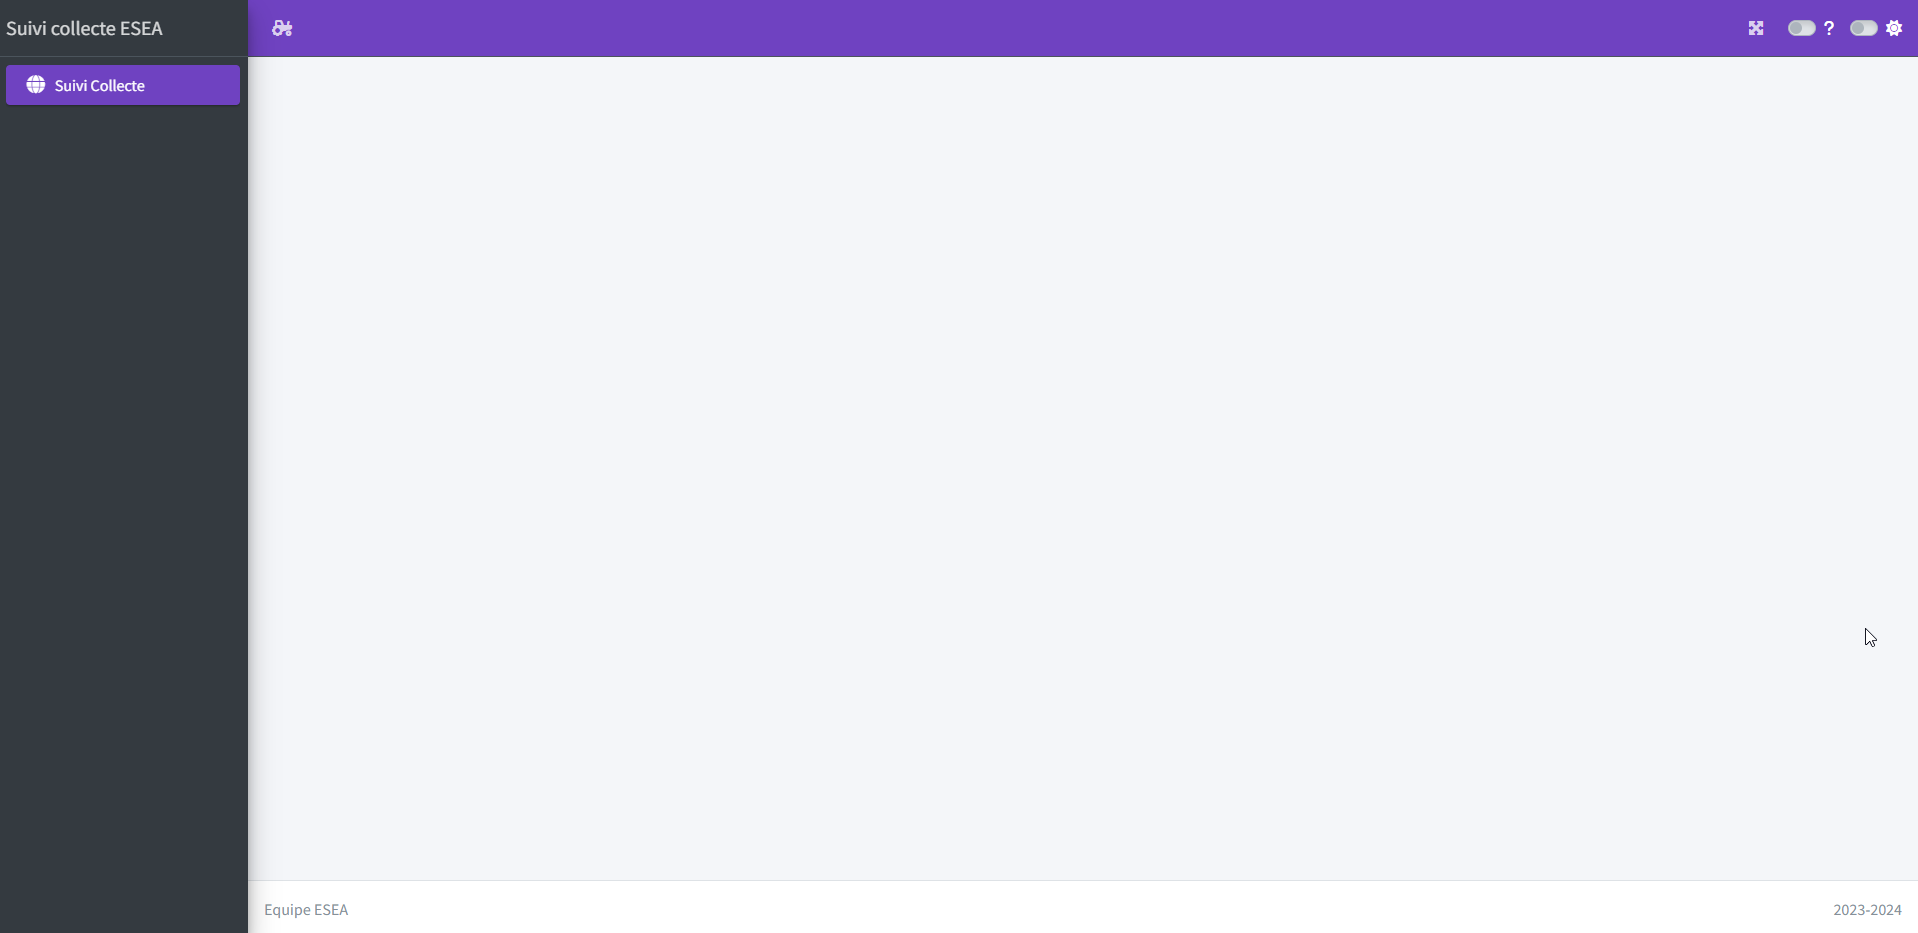
\includegraphics{./images/esea_squelette_vide.png}

\hypertarget{commit-et-push-github}{%
\section{Commit et push Github}\label{commit-et-push-github}}

Avant de passer à la suite, pensez à commiter et pusher votre code.

\hypertarget{cruxe9ation-dune-premiuxe8re-page}{%
\section{Création d'une première
page}\label{cruxe9ation-dune-premiuxe8re-page}}

Maintenant que l'on a notre premier module (première page), nous allons
pouvoir la peupler avec des box. Voir
\protect\hyperlink{ajout-de-box-dans-une-page}{page suivante}

\bookmarksetup{startatroot}

\hypertarget{ajout-de-box-dans-une-page}{%
\chapter{Ajout de box dans une page}\label{ajout-de-box-dans-une-page}}

L'ajout de box dans une page se fait dans le programme
R/mod\_name\_of\_module1\_ui. Dance ce programme il y a 3 parties à
modifier :

\begin{itemize}
\tightlist
\item
  dans l'\textbf{entête} on doit ajouter les packages à importer (ou les
  fonctions des packages),\\
\item
  la fonction \textbf{mod\_name\_of\_module1\_ui} qui va gérer
  l'affichage dans la page : les lignes et les box que l'on ajoute,\\
\item
  la fonction \textbf{mod\_name\_of\_module1\_server} qui permet de
  faire les calculs et les traitements qui seront affichés dans les box.
\end{itemize}

La distiction \emph{ui} et \emph{server} est classique pour toute
application shiny. Voir la
\href{https://shiny.posit.co/r/getstarted/shiny-basics/lesson1/}{documentation
shiny} si besoin.

\hypertarget{accuxe8s-aux-donnuxe9es}{%
\section{Accès aux données}\label{accuxe8s-aux-donnuxe9es}}

Pour créer les box de suivi de la collecte, il faut avoir un accès à la
donnée. Pour rappel la donnée est stockée au format parquet dans le
bucket partagé.

\hypertarget{le-plus-simple-chargement-uxe0-chaque-module}{%
\subsection{Le plus simple : chargement à chaque
module}\label{le-plus-simple-chargement-uxe0-chaque-module}}

Dans chaque module, charger les données avant de lancer les fonction ui
et server :

\begin{Shaded}
\begin{Highlighting}[]
\CommentTok{\#\textquotesingle{} @importFrom aws.s3 s3read\_using}
\CommentTok{\#\textquotesingle{} @importFrom arrow read\_parquet}
\CommentTok{\#\textquotesingle{} @noRd}

\NormalTok{data\_suivi }\OtherTok{\textless{}{-}}\NormalTok{ aws.s3}\SpecialCharTok{::}\FunctionTok{s3read\_using}\NormalTok{(}
  \AttributeTok{FUN =}\NormalTok{ arrow}\SpecialCharTok{::}\NormalTok{read\_parquet,}
  \AttributeTok{object =} \StringTok{"ESEA/suivi.parquet"}\NormalTok{,}
  \AttributeTok{bucket =} \StringTok{"projet{-}suivi{-}collecte{-}masa"}\NormalTok{,}
  \AttributeTok{opts =} \FunctionTok{list}\NormalTok{(}\StringTok{"region"} \OtherTok{=} \StringTok{""}\NormalTok{)}
\NormalTok{)}
\end{Highlighting}
\end{Shaded}

Pour vérifier que l'import des données fonctionne, vous pouvez modifier
le fichier de module de la manière suivante :

\begin{Shaded}
\begin{Highlighting}[]
\NormalTok{mod\_suivi\_collecte\_ui }\OtherTok{\textless{}{-}} \ControlFlowTok{function}\NormalTok{(id)\{}
\NormalTok{  ns }\OtherTok{\textless{}{-}} \FunctionTok{NS}\NormalTok{(id)}
  \FunctionTok{tagList}\NormalTok{(}
\NormalTok{    shiny}\SpecialCharTok{::}\FunctionTok{verbatimTextOutput}\NormalTok{(}\FunctionTok{ns}\NormalTok{(}\StringTok{"data\_test\_load"}\NormalTok{))}
\NormalTok{  )}
\NormalTok{\}}

\NormalTok{mod\_suivi\_collecte\_server }\OtherTok{\textless{}{-}} \ControlFlowTok{function}\NormalTok{(id)\{}
  \FunctionTok{moduleServer}\NormalTok{(id, }\ControlFlowTok{function}\NormalTok{(input, output, session)\{}
\NormalTok{    ns }\OtherTok{\textless{}{-}}\NormalTok{ session}\SpecialCharTok{$}\NormalTok{ns}
\NormalTok{    output}\SpecialCharTok{$}\NormalTok{data\_test\_load }\OtherTok{\textless{}{-}}  \FunctionTok{renderText}\NormalTok{(\{}
\NormalTok{        data }\OtherTok{\textless{}{-}}\NormalTok{ data\_suivi}
        \FunctionTok{nrow}\NormalTok{(data)}
\NormalTok{    \})}
\NormalTok{  \})}
\NormalTok{\}}
\end{Highlighting}
\end{Shaded}

\hypertarget{mieux-charger-les-donnuxe9es-une-seule-fois}{%
\subsection{Mieux : charger les données une seule
fois}\label{mieux-charger-les-donnuxe9es-une-seule-fois}}

Pour être plus propre, on peut charger les données une seule fois en
utilisant la
\href{https://rtask.thinkr.fr/fr/la-communication-entre-modules-et-ses-caprices/}{technique
du petit r}.

Dans le fichier R/app\_server.R il faut créer un r qui soit un
\textbf{reactiveValues}, puis charger les jeux de données dans ce r, et
passer ce r en paramètre des mod\_XXXXX\_server. Exemple :

\begin{Shaded}
\begin{Highlighting}[]
\NormalTok{app\_server }\OtherTok{\textless{}{-}} \ControlFlowTok{function}\NormalTok{(input, output, session) \{}
\NormalTok{  r }\OtherTok{\textless{}{-}} \FunctionTok{reactiveValues}\NormalTok{()}
  \FunctionTok{observe}\NormalTok{(\{}
\NormalTok{    r}\SpecialCharTok{$}\NormalTok{data\_suivi }\OtherTok{\textless{}{-}}\NormalTok{ aws.s3}\SpecialCharTok{::}\FunctionTok{s3read\_using}\NormalTok{(}
       \AttributeTok{FUN =}\NormalTok{ arrow}\SpecialCharTok{::}\NormalTok{read\_parquet,}
        \AttributeTok{object =} \StringTok{"ESEA/suivi.parquet"}\NormalTok{,}
        \AttributeTok{bucket =} \StringTok{"projet{-}suivi{-}collecte{-}masa"}\NormalTok{,}
        \AttributeTok{opts =} \FunctionTok{list}\NormalTok{(}\StringTok{"region"} \OtherTok{=} \StringTok{""}\NormalTok{)}
\NormalTok{        )  }

    

\NormalTok{  \})}
 \CommentTok{\# Your application server logic}
  \FunctionTok{mod\_suivi\_collecte\_server}\NormalTok{(}\StringTok{"suivi\_collecte\_1"}\NormalTok{,r)}
\NormalTok{\}}
\end{Highlighting}
\end{Shaded}

Puis dans le mod\_XXXXX\_ui, il faut mettre à jour la fonction
\textbf{mod\_XXXX\_server} pour intégrer le r. Exemple :

\begin{Shaded}
\begin{Highlighting}[]
\NormalTok{mod\_suivi\_collecte\_ui }\OtherTok{\textless{}{-}} \ControlFlowTok{function}\NormalTok{(id)\{}
\NormalTok{  ns }\OtherTok{\textless{}{-}} \FunctionTok{NS}\NormalTok{(id)}
  \FunctionTok{tagList}\NormalTok{(}
\NormalTok{    shiny}\SpecialCharTok{::}\FunctionTok{verbatimTextOutput}\NormalTok{(}\FunctionTok{ns}\NormalTok{(}\StringTok{"data\_test\_load"}\NormalTok{))}
\NormalTok{  )}
\NormalTok{\}}

\NormalTok{mod\_suivi\_collecte\_server }\OtherTok{\textless{}{-}} \ControlFlowTok{function}\NormalTok{(id, r)\{}
  \FunctionTok{moduleServer}\NormalTok{(id, }\ControlFlowTok{function}\NormalTok{(input, output, session)\{}
\NormalTok{    ns }\OtherTok{\textless{}{-}}\NormalTok{ session}\SpecialCharTok{$}\NormalTok{ns}
\NormalTok{    output}\SpecialCharTok{$}\NormalTok{data\_test\_load }\OtherTok{\textless{}{-}}  \FunctionTok{renderText}\NormalTok{(\{r}\SpecialCharTok{$}\NormalTok{data\_suivi \})}
\NormalTok{  \})}
\NormalTok{\}}
\end{Highlighting}
\end{Shaded}

Pensez ensuite à lancer un \textbf{attachment::att\_amend\_desc()} afin
d'intégrer les packages dans les dépendances.

\hypertarget{ajouter-des-lignes}{%
\section{Ajouter des lignes}\label{ajouter-des-lignes}}

Le principe du body de bs4Dash est de mettre des lignes et dans chaque
ligne mettre des box. Pour ajouter une ligne, c'est très simple, il faut
ajouter un \textbf{fluidRow()} dans l'ui du module (dans le
\textbf{tagList}).

\hypertarget{ajouter-une-box-dinfo-ou-de-valeur}{%
\section{Ajouter une box d'info ou de
valeur}\label{ajouter-une-box-dinfo-ou-de-valeur}}

Côté ui, il faut ajouter une valueBoxOupt ou une infoBoxOutput. Côté
server, il faut créer un renderValueBox ou un renderValueBox.

Attention, en golem pour passer du server à l'ui il faut envoyer
l'output avec un ns(). Par exemple si l'output est ``ma\_value\_box''
alors dans l'ui il faudra appeler
renderValueBox(ns(``ma\_value\_box'')).

Dans l'exemple ci-dessous, on utilise la stratégie du petit r pour que
les données soient utilisées pour tout le site. Dans la partie server,
il faudra mettre le code dans un Observe pour avoir accès aux
reactiveValues du petit r.

Exemple :

\begin{Shaded}
\begin{Highlighting}[]
\NormalTok{mod\_suivi\_collecte\_ui }\OtherTok{\textless{}{-}} \ControlFlowTok{function}\NormalTok{(id)\{}
\NormalTok{  ns }\OtherTok{\textless{}{-}} \FunctionTok{NS}\NormalTok{(id)}
  \FunctionTok{tagList}\NormalTok{(}
    \FunctionTok{fluidRow}\NormalTok{(}
          \FunctionTok{infoBoxOutput}\NormalTok{(}\FunctionTok{ns}\NormalTok{(}\StringTok{"nb\_questionnaires"}\NormalTok{)),}
          \FunctionTok{valueBoxOutput}\NormalTok{(}\FunctionTok{ns}\NormalTok{(}\StringTok{"taux\_collecte"}\NormalTok{)),}
          \FunctionTok{valueBoxOutput}\NormalTok{(}\FunctionTok{ns}\NormalTok{(}\StringTok{"taux\_reponse"}\NormalTok{))}
\NormalTok{        )}
\NormalTok{  )}
\NormalTok{\}}

\NormalTok{mod\_suivi\_collecte\_server }\OtherTok{\textless{}{-}} \ControlFlowTok{function}\NormalTok{(id, r)\{}
  \FunctionTok{moduleServer}\NormalTok{(id, }\ControlFlowTok{function}\NormalTok{(input, output, session)\{}
\NormalTok{    ns }\OtherTok{\textless{}{-}}\NormalTok{ session}\SpecialCharTok{$}\NormalTok{ns}
    \FunctionTok{observe}\NormalTok{(\{}
\NormalTok{      questionnaires\_totaux\_esea }\OtherTok{\textless{}{-}}\NormalTok{ r}\SpecialCharTok{$}\NormalTok{data\_suivi }\SpecialCharTok{\%\textgreater{}\%} \FunctionTok{nrow}\NormalTok{()}
\NormalTok{      questionnaires\_collectes }\OtherTok{\textless{}{-}}\NormalTok{  r}\SpecialCharTok{$}\NormalTok{data\_suivi }\SpecialCharTok{\%\textgreater{}\%} \FunctionTok{filter}\NormalTok{(ETAT\_CONTROLE  }\SpecialCharTok{!=} \DecValTok{1}\NormalTok{) }\SpecialCharTok{\%\textgreater{}\%} \FunctionTok{nrow}\NormalTok{()}
\NormalTok{      questionnaires\_valides }\OtherTok{\textless{}{-}}\NormalTok{  r}\SpecialCharTok{$}\NormalTok{data\_suivi }\SpecialCharTok{\%\textgreater{}\%} \FunctionTok{filter}\NormalTok{(ETAT\_CONTROLE  }\SpecialCharTok{==} \DecValTok{5}\NormalTok{) }\SpecialCharTok{\%\textgreater{}\%} \FunctionTok{nrow}\NormalTok{()}

\NormalTok{      output}\SpecialCharTok{$}\NormalTok{nb\_questionnaires }\OtherTok{\textless{}{-}} \FunctionTok{renderInfoBox}\NormalTok{(\{}
        \FunctionTok{infoBox}\NormalTok{(}
          \AttributeTok{title =} \StringTok{"Nombre total de questionnaires"}\NormalTok{,}
          \AttributeTok{fill =} \ConstantTok{TRUE}\NormalTok{,}
          \AttributeTok{gradient =} \ConstantTok{TRUE}\NormalTok{,}
          \AttributeTok{color =} \StringTok{"info"}\NormalTok{,}
          \AttributeTok{value =}\NormalTok{ questionnaires\_totaux\_esea,}
          \AttributeTok{icon =} \FunctionTok{icon}\NormalTok{(}\StringTok{"paper{-}plane"}\NormalTok{)}
\NormalTok{        )}
\NormalTok{      \})}

\NormalTok{       output}\SpecialCharTok{$}\NormalTok{taux\_collecte }\OtherTok{\textless{}{-}} \FunctionTok{renderValueBox}\NormalTok{(\{}
        \FunctionTok{valueBox}\NormalTok{(}
          \AttributeTok{value =} \FunctionTok{glue}\NormalTok{(}\FunctionTok{round}\NormalTok{(}\DecValTok{100} \SpecialCharTok{*}\NormalTok{(questionnaires\_collectes }\SpecialCharTok{/}\NormalTok{ questionnaires\_totaux\_esea),}\DecValTok{3}\NormalTok{), }\StringTok{\textquotesingle{} \%\textquotesingle{}}\NormalTok{),}
          \AttributeTok{subtitle =} \StringTok{"Taux de collecte (questionnaires qui ne sont plus en état initial)"}\NormalTok{,}
        \AttributeTok{color =} \StringTok{"primary"}\NormalTok{,}
        \AttributeTok{icon =} \FunctionTok{icon}\NormalTok{(}\StringTok{"circle{-}check"}\NormalTok{)}
\NormalTok{        )}
\NormalTok{      \})}

\NormalTok{      output}\SpecialCharTok{$}\NormalTok{taux\_reponse }\OtherTok{\textless{}{-}} \FunctionTok{renderValueBox}\NormalTok{(\{}
        \FunctionTok{valueBox}\NormalTok{(}
          \AttributeTok{value =} \FunctionTok{glue}\NormalTok{(}\FunctionTok{round}\NormalTok{(}\DecValTok{100} \SpecialCharTok{*}\NormalTok{(questionnaires\_valides }\SpecialCharTok{/}\NormalTok{ questionnaires\_totaux\_esea),}\DecValTok{3}\NormalTok{), }\StringTok{\textquotesingle{} \%\textquotesingle{}}\NormalTok{),}
          \AttributeTok{subtitle =} \StringTok{"Taux de réponse (questionnaires validés)"}\NormalTok{,}
        \AttributeTok{color =} \StringTok{"teal"}\NormalTok{,}
        \AttributeTok{icon =} \FunctionTok{icon}\NormalTok{(}\StringTok{"thumbs{-}up"}\NormalTok{)}
\NormalTok{        )}
\NormalTok{      \})}

\NormalTok{    \})}

\NormalTok{  \})}
\NormalTok{\}}
\end{Highlighting}
\end{Shaded}

\hypertarget{ajouter-une-box-de-contenu}{%
\section{Ajouter une box de contenu}\label{ajouter-une-box-de-contenu}}

Pour ajouter des box de contenus, on fera la même chose que pour les box
de valeur / info : on ajoute une fluidRow et on y met une ou plusieurs
\textbf{bs4Dash::box}. Parmi les paramètres de la box on pourra gérer le
titre, le statut (la couleur), la taille en hauteur et en
largeur\ldots{}

\hypertarget{avec-un-graphique}{%
\subsection{Avec un graphique}\label{avec-un-graphique}}

On peut facilement ajouter des graphiques ggplot2. Mais pour un rendu
plus joli sur le web nous préconisons l'utilisation de
\href{https://echarts4r.john-coene.com/}{echarts4r}. Dans une
bs4Dash::box, on ajoutera un echarts4rOutput et dans le server on créera
un renderEcharts4r.

Voici un exemple :

\begin{Shaded}
\begin{Highlighting}[]
\CommentTok{\# côté ui, dans le tagList :}

\FunctionTok{fluidRow}\NormalTok{(}
\NormalTok{      bs4Dash}\SpecialCharTok{::}\FunctionTok{box}\NormalTok{(}
          \AttributeTok{title =} \StringTok{"Avancement de la collecte"}\NormalTok{,}
          \AttributeTok{status =} \StringTok{"orange"}\NormalTok{,}
          \FunctionTok{echarts4rOutput}\NormalTok{(}\FunctionTok{ns}\NormalTok{(}\StringTok{"pie\_questionnaire\_par\_etat"}\NormalTok{))}
\NormalTok{      )}
\NormalTok{    )    }

\CommentTok{\# côté server}
\NormalTok{    output}\SpecialCharTok{$}\NormalTok{pie\_questionnaire\_par\_etat }\OtherTok{\textless{}{-}} \FunctionTok{renderEcharts4r}\NormalTok{(\{}
\NormalTok{       dossier }\OtherTok{\textless{}{-}}\NormalTok{ r}\SpecialCharTok{$}\NormalTok{data\_suivi}
       
\NormalTok{       questionnaire\_par\_etat }\OtherTok{\textless{}{-}}\NormalTok{ dossier }\SpecialCharTok{\%\textgreater{}\%}
         \FunctionTok{count}\NormalTok{(ETAT\_CONTROLE) }\SpecialCharTok{\%\textgreater{}\%}
         \FunctionTok{mutate}\NormalTok{(}
          \AttributeTok{ETAT\_CONTROLE =} \FunctionTok{case\_when}\NormalTok{(}
\NormalTok{            ETAT\_CONTROLE }\SpecialCharTok{==} \DecValTok{1} \SpecialCharTok{\textasciitilde{}} \StringTok{"Non collecté"}\NormalTok{,}
\NormalTok{            ETAT\_CONTROLE }\SpecialCharTok{==} \DecValTok{5} \SpecialCharTok{\textasciitilde{}} \StringTok{"Validé"}\NormalTok{,}
\NormalTok{            ETAT\_CONTROLE }\SpecialCharTok{==} \DecValTok{4} \SpecialCharTok{\textasciitilde{}} \StringTok{"A confirmer"}\NormalTok{,}
\NormalTok{            ETAT\_CONTROLE }\SpecialCharTok{==} \DecValTok{2} \SpecialCharTok{\textasciitilde{}} \StringTok{"A compléter"}\NormalTok{,}
\NormalTok{            ETAT\_CONTROLE }\SpecialCharTok{==} \DecValTok{3} \SpecialCharTok{\textasciitilde{}} \StringTok{"A corriger"}\NormalTok{,}
            \ConstantTok{TRUE} \SpecialCharTok{\textasciitilde{}} \StringTok{"Indéterminé"}
\NormalTok{          )}
\NormalTok{         )}

\NormalTok{       questionnaire\_par\_etat }\SpecialCharTok{\%\textgreater{}\%}
        \FunctionTok{e\_charts}\NormalTok{(ETAT\_CONTROLE) }\SpecialCharTok{\%\textgreater{}\%}
        \FunctionTok{e\_pie}\NormalTok{(n, }\AttributeTok{radius =} \FunctionTok{c}\NormalTok{(}\StringTok{"40\%"}\NormalTok{, }\StringTok{"70\%"}\NormalTok{)) }\SpecialCharTok{|\textgreater{}}
        \FunctionTok{e\_tooltip}\NormalTok{(}\AttributeTok{formatter =}\NormalTok{ htmlwidgets}\SpecialCharTok{::}\FunctionTok{JS}\NormalTok{(}\StringTok{"function(params) \{return params.name + \textquotesingle{}: \textquotesingle{} + params.value;\}"}\NormalTok{))}
\NormalTok{    \})}
\end{Highlighting}
\end{Shaded}

\hypertarget{avec-une-carte}{%
\subsection{Avec une carte}\label{avec-une-carte}}

Pour les cartes, nous préconisons leaflet qui permet de faire des cartes
web zoomable assez chouettes.

Avant tout, il faut charger les fonds de carte. Nous préconisons
l'utilisation de topojson accessible en ligne :

\begin{itemize}
\tightlist
\item
  \href{https://raw.githubusercontent.com/neocarto/resources/master/geometries/France/regions.topojson}{Régions
  de France}
\item
  \href{https://raw.githubusercontent.com/neocarto/resources/master/geometries/France/departements.topojson}{Départements
  de France}
\end{itemize}

Nous les ajoutons au r pour qu'ils soient accessibles dans tous les
modules, en passant par le package \textbf{geojsonio} (à ajouter aux
imports).

Pour que \textbf{geojsonio} fonctionne, il faut installer plusieurs
librairies dans le serveur hébergeant le VSCode. Pour cela il faut
ouvrir un nouveau terminal (un terminal de base, pas un terminal R) et
lancer successivement les commandes :

\begin{Shaded}
\begin{Highlighting}[]
\NormalTok{sudo apt}\OperatorTok{{-}}\NormalTok{get update}
\NormalTok{sudo apt}\OperatorTok{{-}}\NormalTok{get }\OperatorTok{{-}}\NormalTok{y install libudunits2}\OperatorTok{{-}}\NormalTok{dev}
\NormalTok{sudo apt}\OperatorTok{{-}}\NormalTok{get }\OperatorTok{{-}}\NormalTok{y install libproj}\OperatorTok{{-}}\NormalTok{dev}
\NormalTok{sudo apt}\OperatorTok{{-}}\NormalTok{get }\OperatorTok{{-}}\NormalTok{y install libgdal}\OperatorTok{{-}}\NormalTok{dev}
\NormalTok{sudo apt}\OperatorTok{{-}}\NormalTok{get install pandoc}
\end{Highlighting}
\end{Shaded}

Puis on peut ajouter les topojson à notre petit r, dans le fichier
R/app\_server.R :

\begin{Shaded}
\begin{Highlighting}[]
\NormalTok{r}\SpecialCharTok{$}\NormalTok{map\_region }\OtherTok{\textless{}{-}}\NormalTok{ geojsonio}\SpecialCharTok{::}\FunctionTok{topojson\_read}\NormalTok{(}\StringTok{"https://raw.githubusercontent.com/neocarto/resources/master/geometries/France/regions.topojson"}\NormalTok{)}

\NormalTok{r}\SpecialCharTok{$}\NormalTok{map\_departements }\OtherTok{\textless{}{-}}\NormalTok{ geojsonio}\SpecialCharTok{::}\FunctionTok{topojson\_read}\NormalTok{(}\StringTok{"https://raw.githubusercontent.com/neocarto/resources/master/geometries/France/departements.topojson"}\NormalTok{)}
\end{Highlighting}
\end{Shaded}

Nous pouvons maintenant ajouter une box contenant un
\textbf{leafletOutput} et créer la foncion \textbf{renderLeaflet} côté
serveur. Voici un exemple de carte choroplèthe par région :

\begin{Shaded}
\begin{Highlighting}[]
\DocumentationTok{\#\#\# dans la partie ui}
\FunctionTok{fluidRow}\NormalTok{(}
\NormalTok{      bs4Dash}\SpecialCharTok{::}\FunctionTok{box}\NormalTok{(}
          \AttributeTok{title =} \StringTok{"Avancement de la collecte"}\NormalTok{,}
          \AttributeTok{status =} \StringTok{"indigo"}\NormalTok{,}
          \FunctionTok{leafletOutput}\NormalTok{(}\FunctionTok{ns}\NormalTok{(}\StringTok{"map\_taux\_collecte"}\NormalTok{))}
\NormalTok{      )}
\NormalTok{    )    }


\DocumentationTok{\#\#\# dans la partie server}

\NormalTok{output}\SpecialCharTok{$}\NormalTok{map\_taux\_collecte }\OtherTok{\textless{}{-}} \FunctionTok{renderLeaflet}\NormalTok{(\{}
        
\NormalTok{        suivi\_par\_region }\OtherTok{\textless{}{-}}\NormalTok{ r}\SpecialCharTok{$}\NormalTok{data\_suivi }\SpecialCharTok{\%\textgreater{}\%}
          \FunctionTok{mutate}\NormalTok{(}\AttributeTok{collecte =} \FunctionTok{ifelse}\NormalTok{(ETAT\_CONTROLE }\SpecialCharTok{==} \DecValTok{1}\NormalTok{ , }\StringTok{"Non collecté"}\NormalTok{, }\StringTok{\textquotesingle{}Collecté\textquotesingle{}}\NormalTok{)) }\SpecialCharTok{\%\textgreater{}\%}
          \FunctionTok{group\_by}\NormalTok{(collecte, REP\_CODE\_REG\_1) }\SpecialCharTok{\%\textgreater{}\%}
          \FunctionTok{count}\NormalTok{() }\SpecialCharTok{\%\textgreater{}\%}
          \FunctionTok{pivot\_wider}\NormalTok{(}\AttributeTok{names\_from =}\NormalTok{ collecte, }\AttributeTok{values\_from =}\NormalTok{ n,  }\AttributeTok{values\_fill =} \DecValTok{0}\NormalTok{) }\SpecialCharTok{\%\textgreater{}\%}
          \FunctionTok{filter}\NormalTok{(}\SpecialCharTok{!}\FunctionTok{is.na}\NormalTok{(REP\_CODE\_REG\_1)) }\SpecialCharTok{\%\textgreater{}\%}
          \FunctionTok{mutate}\NormalTok{(}\AttributeTok{total =}\NormalTok{ Collecté }\SpecialCharTok{+} \StringTok{\textasciigrave{}}\AttributeTok{Non collecté}\StringTok{\textasciigrave{}}\NormalTok{) }\SpecialCharTok{\%\textgreater{}\%}
          \FunctionTok{mutate}\NormalTok{(}\AttributeTok{taux\_collecte =}\NormalTok{ Collecté}\SpecialCharTok{/}\NormalTok{total)}

\NormalTok{        data\_map }\OtherTok{\textless{}{-}}\NormalTok{ r}\SpecialCharTok{$}\NormalTok{map\_regions }\SpecialCharTok{\%\textgreater{}\%}
          \FunctionTok{left\_join}\NormalTok{(suivi\_par\_region, }\AttributeTok{by =} \FunctionTok{c}\NormalTok{(}\StringTok{"REG"} \OtherTok{=} \StringTok{"REP\_CODE\_REG\_1"}\NormalTok{))}

\NormalTok{        pal }\OtherTok{\textless{}{-}} \FunctionTok{colorNumeric}\NormalTok{(}\StringTok{"RdYlGn"}\NormalTok{, }\ConstantTok{NULL}\NormalTok{)}

\NormalTok{        leaflet}\SpecialCharTok{::}\FunctionTok{leaflet}\NormalTok{(data\_map) }\SpecialCharTok{\%\textgreater{}\%}
          \FunctionTok{addPolygons}\NormalTok{(}\AttributeTok{stroke =} \ConstantTok{FALSE}\NormalTok{, }
              \AttributeTok{smoothFactor =} \FloatTok{0.3}\NormalTok{, }
              \AttributeTok{fillOpacity =} \DecValTok{1}\NormalTok{,}
              \AttributeTok{fillColor =} \SpecialCharTok{\textasciitilde{}}\FunctionTok{pal}\NormalTok{(taux\_collecte),}
              \AttributeTok{label =} \SpecialCharTok{\textasciitilde{}}\FunctionTok{paste0}\NormalTok{(Name, }\StringTok{": "}\NormalTok{,}
                              \FunctionTok{round}\NormalTok{(}\DecValTok{100} \SpecialCharTok{*}\NormalTok{ taux\_collecte,}\DecValTok{0}\NormalTok{),}
                              \StringTok{" \% / "}\NormalTok{,Collecté,}\StringTok{" collectés pour "}\NormalTok{, total,}\StringTok{" au total."}\NormalTok{)) }\SpecialCharTok{\%\textgreater{}\%}
              \FunctionTok{addLegend}\NormalTok{(}\AttributeTok{pal =}\NormalTok{ pal, }\AttributeTok{values =} \SpecialCharTok{\textasciitilde{}}\FunctionTok{round}\NormalTok{(}\DecValTok{100}\SpecialCharTok{*}\NormalTok{taux\_collecte,}\DecValTok{0}\NormalTok{), }\AttributeTok{title =} \StringTok{"Taux de collecte"}\NormalTok{,}
                    \AttributeTok{opacity =} \DecValTok{1}\NormalTok{, }\AttributeTok{position =} \StringTok{"bottomright"}\NormalTok{, }\AttributeTok{na.label=} \StringTok{"?"}\NormalTok{,}\AttributeTok{labFormat =} \FunctionTok{labelFormat}\NormalTok{(}\AttributeTok{suffix=}\StringTok{" \%"}\NormalTok{))}

\NormalTok{    \})}
\end{Highlighting}
\end{Shaded}

\hypertarget{avec-un-tableau}{%
\subsection{Avec un tableau}\label{avec-un-tableau}}

Il est possible d'afficher des tableaux dans les box. Nous préconisons
l'utilisation du package DT (à ajouter dans les imports) : côté ui on
aura un \textbf{dataTableOutput} et côté serveur un
\textbf{renderDataTable}. Il est possible grâce à ce package et à des
extensions indiquées dans la fonction datatable d'ajouter des scollers
et des boutons (par exemple : export PDF, xlsx, csv\ldots).

Voici un exemple :

\begin{Shaded}
\begin{Highlighting}[]
\CommentTok{\# Côté UI}
\FunctionTok{fluidRow}\NormalTok{(}
\NormalTok{          bs4Dash}\SpecialCharTok{::}\FunctionTok{box}\NormalTok{(}\AttributeTok{title =} \StringTok{"Liste des dossiers"}\NormalTok{,}
                   \AttributeTok{status =} \StringTok{"orange"}\NormalTok{,}
\NormalTok{                   DT}\SpecialCharTok{::}\FunctionTok{dataTableOutput}\NormalTok{(}\FunctionTok{ns}\NormalTok{(}\StringTok{"table\_dossiers"}\NormalTok{)),}
                   \AttributeTok{width =} \DecValTok{12}\NormalTok{,}
                   \AttributeTok{height =} \StringTok{"900px"}
\NormalTok{      )}
\NormalTok{      )}

\CommentTok{\# Côté Server}
\NormalTok{     output}\SpecialCharTok{$}\NormalTok{table\_dossiers }\OtherTok{\textless{}{-}}
\NormalTok{         DT}\SpecialCharTok{::}\FunctionTok{renderDataTable}\NormalTok{(}
\NormalTok{            dossier }\OtherTok{\textless{}{-}}\NormalTok{ r}\SpecialCharTok{$}\NormalTok{data\_suivi }\SpecialCharTok{\%\textgreater{}\%}
                \FunctionTok{datatable}\NormalTok{(}\AttributeTok{rownames =} \ConstantTok{FALSE}\NormalTok{,}
                 \AttributeTok{extensions =} \FunctionTok{c}\NormalTok{(}\StringTok{"Scroller"}\NormalTok{, }\StringTok{"FixedColumns"}\NormalTok{, }\StringTok{"Buttons"}\NormalTok{, }\StringTok{"Select"}\NormalTok{),}
                 \AttributeTok{selection =} \StringTok{\textquotesingle{}none\textquotesingle{}}\NormalTok{,}
                   \AttributeTok{filter =} \FunctionTok{list}\NormalTok{(}\AttributeTok{position =} \StringTok{\textquotesingle{}top\textquotesingle{}}\NormalTok{,}
                      \AttributeTok{clear =} \ConstantTok{TRUE}\NormalTok{,}
                      \AttributeTok{plain =} \ConstantTok{FALSE}
\NormalTok{                   ),}
                 \AttributeTok{options =} \FunctionTok{list}\NormalTok{(}
                   \AttributeTok{dom =} \StringTok{"Bfrtip"}\NormalTok{,}
                   \CommentTok{\# scroll :}
                   \AttributeTok{scrollY =} \DecValTok{750}\NormalTok{, }\AttributeTok{scrollX =} \DecValTok{400}\NormalTok{, }\AttributeTok{scroller =} \ConstantTok{TRUE}\NormalTok{,}
                   \CommentTok{\# fixer les colonnes :}
                   \AttributeTok{fixedColumns =} \FunctionTok{list}\NormalTok{(}\AttributeTok{leftColumns =} \DecValTok{1}\NormalTok{),}
                   \CommentTok{\# selection :}
                   \AttributeTok{select =} \FunctionTok{list}\NormalTok{(}\AttributeTok{style =} \StringTok{\textquotesingle{}os\textquotesingle{}}\NormalTok{, }\AttributeTok{items =} \StringTok{\textquotesingle{}row\textquotesingle{}}\NormalTok{),}
                   \AttributeTok{buttons =} \FunctionTok{c}\NormalTok{(}
                     \CommentTok{\# enregistrements}
                      \StringTok{\textquotesingle{}csv\textquotesingle{}}\NormalTok{, }\StringTok{\textquotesingle{}excel\textquotesingle{}}\NormalTok{, }\StringTok{\textquotesingle{}pdf\textquotesingle{}}\NormalTok{,}
                     \CommentTok{\# selection des elements}
                     \StringTok{\textquotesingle{}selectAll\textquotesingle{}}\NormalTok{, }\StringTok{\textquotesingle{}selectNone\textquotesingle{}}\NormalTok{, }\StringTok{\textquotesingle{}selectRows\textquotesingle{}}
\NormalTok{                   )}
\NormalTok{                 )}
\NormalTok{                )}
\NormalTok{         )}
\end{Highlighting}
\end{Shaded}

\hypertarget{ajout-de-boutons}{%
\subsection{Ajout de boutons}\label{ajout-de-boutons}}

Dans une box il est possible d'ajouter des boutons afin de changer le
rendu de la carte ou du graphique. Par exemple on a une carte
d'avancement de collecte par région. On pourrait mettre un bouton pour
afficher la carte par département. Nous préconisons l'utilisation de
\href{https://shinyapps.dreamrs.fr/shinyWidgets/}{shinyWidgets} qui
offre des composants assez ergonomiques.

Le code devra être mis dans la partie ui, et récupérer dans la partie
server pour faire évoluer l'affichage. Prenons l'exemple d'un bouton
région / département pour l'affichage d'une carte.

\begin{Shaded}
\begin{Highlighting}[]
\CommentTok{\# Côté UI}

\NormalTok{      bs4Dash}\SpecialCharTok{::}\FunctionTok{box}\NormalTok{(}
          \AttributeTok{title =} \StringTok{"Avancement de la collecte"}\NormalTok{,}
          \AttributeTok{status =} \StringTok{"indigo"}\NormalTok{,}
\NormalTok{          shinyWidgets}\SpecialCharTok{::}\FunctionTok{awesomeRadio}\NormalTok{(}
            \AttributeTok{inputId =} \FunctionTok{ns}\NormalTok{(}\StringTok{"map\_region\_departement"}\NormalTok{), }\DocumentationTok{\#\#\#\# Attention : ne pas oublier le ns()}
            \AttributeTok{label =} \ConstantTok{NULL}\NormalTok{, }
            \AttributeTok{choices =} \FunctionTok{c}\NormalTok{(}\StringTok{"Région"}\NormalTok{, }\StringTok{"Département"}\NormalTok{),}
            \AttributeTok{selected =} \StringTok{"Région"}\NormalTok{,}
            \AttributeTok{inline =} \ConstantTok{TRUE}\NormalTok{,}
            \AttributeTok{status =} \StringTok{"success"}
\NormalTok{          ),}
          \FunctionTok{leafletOutput}\NormalTok{(}\FunctionTok{ns}\NormalTok{(}\StringTok{"map\_taux\_collecte"}\NormalTok{))}
\NormalTok{      )}

\CommentTok{\# Côté server}
\end{Highlighting}
\end{Shaded}

\hypertarget{utilisation-de-la-fenuxeatre-pliable-de-droite}{%
\subsection{Utilisation de la fenêtre pliable de
droite}\label{utilisation-de-la-fenuxeatre-pliable-de-droite}}

\emph{A compléter}

\bookmarksetup{startatroot}

\hypertarget{suxe9curisation-de-lapplication}{%
\chapter{Sécurisation de
l'application}\label{suxe9curisation-de-lapplication}}

Nous ajoutons une couche de sécurité au site de suivi de collecte grâce
au package \textbf{shinyManager}. Les utilisateurs s'authentifieront via
un identifiant et à un mot de passe que vous définirez par ailleurs.

\hypertarget{test-avec-un-identifiant-mot-de-passe-en-dur}{%
\section{Test avec un identifiant / mot de passe en
dur}\label{test-avec-un-identifiant-mot-de-passe-en-dur}}

Il faut modifier le fichier R/app\_server.R :

\begin{Shaded}
\begin{Highlighting}[]
\CommentTok{\#\textquotesingle{} @import shiny}
\CommentTok{\#\textquotesingle{} @import shinymanager}
\CommentTok{\#\textquotesingle{} @noRd}

\NormalTok{app\_server }\OtherTok{\textless{}{-}} \ControlFlowTok{function}\NormalTok{(input, output, session) \{}
  \CommentTok{\# Your application server logic}
\NormalTok{  res\_auth }\OtherTok{\textless{}{-}}\NormalTok{ shinymanager}\SpecialCharTok{::}\FunctionTok{secure\_server}\NormalTok{(}
    \AttributeTok{check\_credentials =}\NormalTok{ shinymanager}\SpecialCharTok{::}\FunctionTok{check\_credentials}\NormalTok{(}
      \FunctionTok{data.frame}\NormalTok{(}
        \AttributeTok{user =} \FunctionTok{c}\NormalTok{(}\StringTok{"id"}\NormalTok{), }\CommentTok{\# mandatory}
        \AttributeTok{password =} \FunctionTok{c}\NormalTok{(}\StringTok{"123456"}\NormalTok{), }\CommentTok{\# mandatory}
        \AttributeTok{start =} \ConstantTok{NA}\NormalTok{, }\CommentTok{\# optinal (all others)}
        \AttributeTok{expire =} \ConstantTok{NA}\NormalTok{,}
        \AttributeTok{admin =} \FunctionTok{c}\NormalTok{(}\ConstantTok{FALSE}\NormalTok{),}
        \AttributeTok{comment =} \StringTok{"Simple and secure authentification mechanism}
\StringTok{  for single ‘Shiny’ applications."}\NormalTok{,}
        \AttributeTok{stringsAsFactors =} \ConstantTok{FALSE}
\NormalTok{      )}
\NormalTok{    )}
\NormalTok{  )}

  \CommentTok{\# liste de vos modules}
  \FunctionTok{mod\_module1\_server}\NormalTok{(}\StringTok{"module1\_1"}\NormalTok{)}
  \FunctionTok{mod\_module2\_server}\NormalTok{(}\StringTok{"module2\_1"}\NormalTok{)}
\NormalTok{\}}
\end{Highlighting}
\end{Shaded}

Puis vous modifiez le fichier R/run\_app.R pour modifier l'ui :

\begin{Shaded}
\begin{Highlighting}[]
\NormalTok{run\_app }\OtherTok{\textless{}{-}} \ControlFlowTok{function}\NormalTok{(}
  \AttributeTok{onStart =} \ConstantTok{NULL}\NormalTok{,}
  \AttributeTok{options =} \FunctionTok{list}\NormalTok{(),}
  \AttributeTok{enableBookmarking =} \ConstantTok{NULL}\NormalTok{,}
  \AttributeTok{uiPattern =} \StringTok{"/"}\NormalTok{,}
\NormalTok{  ...}
\NormalTok{) \{}
  \FunctionTok{with\_golem\_options}\NormalTok{(}
    \AttributeTok{app =} \FunctionTok{shinyApp}\NormalTok{(}
      \AttributeTok{ui =}\NormalTok{ shinymanager}\SpecialCharTok{::}\FunctionTok{secure\_app}\NormalTok{(app\_ui, }\AttributeTok{language =} \StringTok{"fr"}\NormalTok{),}
      \AttributeTok{server =}\NormalTok{ app\_server,}
      \AttributeTok{onStart =}\NormalTok{ onStart,}
      \AttributeTok{options =}\NormalTok{ options,}
      \AttributeTok{enableBookmarking =}\NormalTok{ enableBookmarking,}
      \AttributeTok{uiPattern =}\NormalTok{ uiPattern}
\NormalTok{    ),}
    \AttributeTok{golem\_opts =} \FunctionTok{list}\NormalTok{(...)}
\NormalTok{  )}
\NormalTok{\}}
\end{Highlighting}
\end{Shaded}

Vous relancez l'application et vous verrez un écran d'authentification.
Saisissez votre identifiant et mot de passe.

\hypertarget{passage-avec-des-secrets-guxe9ruxe9s-par-le-datalab}{%
\section{Passage avec des secrets gérés par le
datalab}\label{passage-avec-des-secrets-guxe9ruxe9s-par-le-datalab}}

Il faut modifier le fichier R/app\_server.R :

\begin{Shaded}
\begin{Highlighting}[]
\CommentTok{\#\textquotesingle{} @import shiny}
\CommentTok{\#\textquotesingle{} @import shinymanager}
\CommentTok{\#\textquotesingle{} @noRd}

\NormalTok{app\_server }\OtherTok{\textless{}{-}} \ControlFlowTok{function}\NormalTok{(input, output, session) \{}
  \CommentTok{\# Your application server logic}
\NormalTok{  res\_auth }\OtherTok{\textless{}{-}}\NormalTok{ shinymanager}\SpecialCharTok{::}\FunctionTok{secure\_server}\NormalTok{(}
    \AttributeTok{check\_credentials =}\NormalTok{ shinymanager}\SpecialCharTok{::}\FunctionTok{check\_credentials}\NormalTok{(}
      \FunctionTok{data.frame}\NormalTok{(}
        \AttributeTok{user =} \FunctionTok{c}\NormalTok{(}\FunctionTok{Sys.getenv}\NormalTok{(}\StringTok{"LOGIN\_SITE\_1"}\NormalTok{), }\FunctionTok{Sys.getenv}\NormalTok{(}\StringTok{"LOGIN\_SITE\_2"}\NormalTok{)), }\CommentTok{\# mandatory}
        \AttributeTok{password =} \FunctionTok{c}\NormalTok{(}\FunctionTok{Sys.getenv}\NormalTok{(}\StringTok{"MDP\_SITE\_2"}\NormalTok{), }\FunctionTok{Sys.getenv}\NormalTok{(}\StringTok{"MDP\_SITE\_2"}\NormalTok{)), }\CommentTok{\# mandatory}
        \AttributeTok{start =} \ConstantTok{NA}\NormalTok{, }
        \AttributeTok{expire =} \FunctionTok{c}\NormalTok{(}\ConstantTok{NA}\NormalTok{, }\ConstantTok{NA}\NormalTok{),}
        \AttributeTok{admin =} \FunctionTok{c}\NormalTok{(}\ConstantTok{FALSE}\NormalTok{, }\ConstantTok{FALSE}\NormalTok{),}
        \AttributeTok{comment =} \StringTok{"Simple and secure authentification mechanism}
\StringTok{  for single ‘Shiny’ applications."}\NormalTok{,}
        \AttributeTok{stringsAsFactors =} \ConstantTok{FALSE}
\NormalTok{      )}
\NormalTok{    )}
\NormalTok{  )}

  \CommentTok{\# liste de vos modules}
  \FunctionTok{mod\_module1\_server}\NormalTok{(}\StringTok{"module1\_1"}\NormalTok{)}
  \FunctionTok{mod\_module2\_server}\NormalTok{(}\StringTok{"module2\_1"}\NormalTok{)}
\NormalTok{\}}
\end{Highlighting}
\end{Shaded}

\bookmarksetup{startatroot}

\hypertarget{duxe9ploiement-de-lapplication}{%
\chapter{Déploiement de
l'application}\label{duxe9ploiement-de-lapplication}}

On a réussi à obtenir une première version du site de suivi de collecte.
Maintenant passons à la publication sur internet de notre site. Le
principe est le suivant :

\begin{itemize}
\tightlist
\item
  l'application shiny est transformée en R package grâce à golem, avec
  toutes ces dépendances;\\
\item
  elle est mise dans un conteneur qu'on appelle Docker;\\
\item
  le docker est déposé dans un site de stockage des dockers :
  dockerHub;\\
\item
  le docker est déployé sur le datalab (grâce à Kubernetes)
\end{itemize}

\hypertarget{vuxe9rification-du-packaging-du-r-package}{%
\section{Vérification du packaging du R
package}\label{vuxe9rification-du-packaging-du-r-package}}

Pour créer le Docker il faut s'assure que le R package puisse bien se
créer. Pour cela, on lancera un \textbf{attachment::att\_amend\_desc()}
puis on lancera la commande : \textbf{devtools::check()}.

S'il y a une Error, il faut absolument la corriger avant de passer à la
suite. S'il n'y a que des warnings et des notes, c'est moins grave, on
peut passer à la suite.

\hypertarget{cruxe9ation-du-docker}{%
\section{Création du Docker}\label{cruxe9ation-du-docker}}

Pour créer le docker il y a 2 fichiers à ajouter à la racine du
suivi\_collecte\_XXX :

\begin{itemize}
\tightlist
\item
  un fichier Dockerfile (sans extension) : c'est une liste de commandes
  permettant de créer le Docker,\\
\item
  un fichier .github/workflows/ci.yaml : c'est un fichier qui permet
  faire l'intégration continue (ci) dans github. A chaque push dans
  Github, un flux de travail (Actions en github) est lancé. Dans notre
  cas ce ci permet de construire le Docker sur la base du fichier Docker
  et de l'envoyer dans DockerHub.
\end{itemize}

\hypertarget{dockerfile}{%
\subsection{Dockerfile}\label{dockerfile}}

Voici à quoi doit ressembler le fichier Dockerfile (a priori vous n'avez
rien à modifier) :

\begin{Shaded}
\begin{Highlighting}[]
\CommentTok{\# Base image}
\NormalTok{FROM rocker}\OperatorTok{/}\NormalTok{shiny:}\FloatTok{4.1.2}

\CommentTok{\# Install required linux librairies}
\NormalTok{RUN apt}\OperatorTok{{-}}\NormalTok{get update }\OperatorTok{{-}}\NormalTok{y }\OperatorTok{\&\&} \OperatorTok{\textbackslash{}}
\NormalTok{    apt}\OperatorTok{{-}}\NormalTok{get install }\OperatorTok{{-}}\NormalTok{y }\OperatorTok{{-}{-}}\NormalTok{no}\OperatorTok{{-}}\NormalTok{install}\OperatorTok{{-}}\NormalTok{recommends libpq}\OperatorTok{{-}}\NormalTok{dev }\OperatorTok{\textbackslash{}}
\NormalTok{                                               libssl}\OperatorTok{{-}}\NormalTok{dev }\OperatorTok{\textbackslash{}}
\NormalTok{                                               libxml2}\OperatorTok{{-}}\NormalTok{dev }\OperatorTok{\textbackslash{}}
\NormalTok{                                               gdal}\OperatorTok{{-}}\BuiltInTok{bin} \OperatorTok{\textbackslash{}}
\NormalTok{                                               libgdal}\OperatorTok{{-}}\NormalTok{dev }\OperatorTok{\textbackslash{}}
\NormalTok{                                               libjq}\OperatorTok{{-}}\NormalTok{dev }\OperatorTok{\textbackslash{}}
\NormalTok{                                               libudunits2}\OperatorTok{{-}}\NormalTok{dev }

\NormalTok{RUN R }\OperatorTok{{-}}\NormalTok{e }\StringTok{"install.packages(\textquotesingle{}shiny\textquotesingle{}, repos=\textquotesingle{}https://cran.rstudio.com/\textquotesingle{})"}
\NormalTok{RUN R }\OperatorTok{{-}}\NormalTok{e }\StringTok{"install.packages(\textquotesingle{}golem\textquotesingle{}, repos=\textquotesingle{}https://cran.rstudio.com/\textquotesingle{})"}

\CommentTok{\# Install R package and its dependencies}
\NormalTok{RUN install2.r remotes}
\NormalTok{COPY suiviCollecte}\OperatorTok{/}\NormalTok{ .}\OperatorTok{/}\NormalTok{suiviCollecte}
\NormalTok{RUN Rscript }\OperatorTok{{-}}\NormalTok{e }\StringTok{\textquotesingle{}remotes::install\_deps("./suiviCollecte")\textquotesingle{}}
\NormalTok{RUN Rscript }\OperatorTok{{-}}\NormalTok{e }\StringTok{\textquotesingle{}install.packages("./suiviCollecte", repos = NULL, type="source")\textquotesingle{}}

\CommentTok{\# Expose port where shiny app will broadcast}
\NormalTok{ARG SHINY\_PORT}\OperatorTok{=}\DecValTok{3838}
\NormalTok{EXPOSE $SHINY\_PORT}
\NormalTok{RUN echo }\StringTok{"local(\{options(shiny.port = $}\SpecialCharTok{\{SHINY\_PORT\}}\StringTok{, shiny.host = \textquotesingle{}0.0.0.0\textquotesingle{})\})"} \OperatorTok{\textgreater{}\textgreater{}} \OperatorTok{/}\NormalTok{usr}\OperatorTok{/}\NormalTok{local}\OperatorTok{/}\NormalTok{lib}\OperatorTok{/}\NormalTok{R}\OperatorTok{/}\NormalTok{etc}\OperatorTok{/}\NormalTok{Rprofile.site}

\CommentTok{\# Endpoint}
\NormalTok{CMD [}\StringTok{"Rscript"}\NormalTok{, }\StringTok{"{-}e"}\NormalTok{, }\StringTok{"suiviCollecte::run\_app()"}\NormalTok{]}
\end{Highlighting}
\end{Shaded}

\hypertarget{cruxe9ation-dun-repository-sur-dockerhub}{%
\subsection{Création d'un repository sur
DockerHub}\label{cruxe9ation-dun-repository-sur-dockerhub}}

Pour pouvoir récupérer le Docker du site de suivi, il faut créer un
repository sur DockerHub :
\href{https://hub.docker.com/repository/create}{Create repository}

\hypertarget{githubworkflowsci.yaml}{%
\subsection{.github/workflows/ci.yaml}\label{githubworkflowsci.yaml}}

Voici à quoi doit ressembler le fichier ci.yaml (il faut modifier le
\textbf{anaeldelorme/suivicollecteexf} où anaeldelorme est le nom
d'utilisateur du dockerHub et suivicollecteexf le nom du repository
DockerHub créé juste avant) :

\begin{Shaded}
\begin{Highlighting}[]
\NormalTok{name: Dockerize}

\NormalTok{on:}
\NormalTok{  push:}
\NormalTok{    tags:}
      \OperatorTok{{-}} \StringTok{"*"}
\NormalTok{    branches:}
      \OperatorTok{{-}}\NormalTok{ main}

\NormalTok{jobs:}
\NormalTok{  docker:}
\NormalTok{    runs}\OperatorTok{{-}}\NormalTok{on: ubuntu}\OperatorTok{{-}}\NormalTok{latest}
\NormalTok{    steps:}
      \OperatorTok{{-}}\NormalTok{ uses: actions}\OperatorTok{/}\NormalTok{checkout}\OperatorTok{@}\NormalTok{v2}
      \OperatorTok{{-}}\NormalTok{ name: Docker meta}
        \BuiltInTok{id}\NormalTok{: docker\_meta}
\NormalTok{        uses: docker}\OperatorTok{/}\NormalTok{metadata}\OperatorTok{{-}}\NormalTok{action}\OperatorTok{@}\NormalTok{v3}
        \ControlFlowTok{with}\NormalTok{:}
\NormalTok{          images: anaeldelorme}\OperatorTok{/}\NormalTok{suivicollecteXXX}
      \OperatorTok{{-}}\NormalTok{ name: Set up QEMU}
\NormalTok{        uses: docker}\OperatorTok{/}\NormalTok{setup}\OperatorTok{{-}}\NormalTok{qemu}\OperatorTok{{-}}\NormalTok{action}\OperatorTok{@}\NormalTok{v1}
      \OperatorTok{{-}}\NormalTok{ name: Set up Docker Buildx}
\NormalTok{        uses: docker}\OperatorTok{/}\NormalTok{setup}\OperatorTok{{-}}\NormalTok{buildx}\OperatorTok{{-}}\NormalTok{action}\OperatorTok{@}\NormalTok{v1}
      \OperatorTok{{-}}\NormalTok{ name: Login to DockerHub}
        \ControlFlowTok{if}\NormalTok{: github.event\_name }\OperatorTok{!=} \StringTok{\textquotesingle{}pull\_request\textquotesingle{}}
\NormalTok{        uses: docker}\OperatorTok{/}\NormalTok{login}\OperatorTok{{-}}\NormalTok{action}\OperatorTok{@}\NormalTok{v1}
        \ControlFlowTok{with}\NormalTok{:}
\NormalTok{          username: $\{\{ secrets.DOCKERHUB\_USERNAME \}\}}
\NormalTok{          password: $\{\{ secrets.DOCKERHUB\_TOKEN \}\}}
      \OperatorTok{{-}}\NormalTok{ name: Build }\KeywordTok{and}\NormalTok{ push}
\NormalTok{        uses: docker}\OperatorTok{/}\NormalTok{build}\OperatorTok{{-}}\NormalTok{push}\OperatorTok{{-}}\NormalTok{action}\OperatorTok{@}\NormalTok{v2}
        \ControlFlowTok{with}\NormalTok{:}
\NormalTok{          context: .}
          \BuiltInTok{file}\NormalTok{: .}\OperatorTok{/}\NormalTok{Dockerfile}
\NormalTok{          push: $\{\{ github.event\_name }\OperatorTok{!=} \StringTok{\textquotesingle{}pull\_request\textquotesingle{}}\NormalTok{ \}\}}
\NormalTok{          tags: }\OperatorTok{|}
\NormalTok{            $\{\{ steps.docker\_meta.outputs.tags \}\}}
\NormalTok{            $\{\{ github.ref }\OperatorTok{==} \StringTok{\textquotesingle{}refs/heads/main\textquotesingle{}} \OperatorTok{\&\&} \StringTok{\textquotesingle{}anaeldelorme/suivicollecteXXX:latest\textquotesingle{}}\NormalTok{ \}\}}
\NormalTok{          labels: $\{\{ steps.docker\_meta.outputs.labels \}\}}
      \OperatorTok{{-}}\NormalTok{ name: Image digest}
\NormalTok{        run: echo $\{\{ steps.docker\_build.outputs.digest \}\}}
\end{Highlighting}
\end{Shaded}

\hypertarget{gestion-des-secrets-dockerhub}{%
\subsection{Gestion des secrets
DockerHub}\label{gestion-des-secrets-dockerhub}}

Comme vous pouvez le voir dans le code, le dépôt sur le DockerHub est
possible parce qu'on passe les variables secrets.DOCKERHUB\_USERNAME et
secrets.DOCKERHUB\_TOKEN. Il convient donc de générer un token dockerhub
:
\href{https://docs.docker.com/security/for-developers/access-tokens/\#create-an-access-token}{Procédure
pour créer un token dockerHub}.

Ensuite il faut mettre le username c'est à dire votre adresse mail
(DOCKERHUB\_USERNAME) et le token (DOCKERHUB\_TOKEN) comme secret du
répertoire Github. Tout est expliqué ici :
\href{https://docs.github.com/en/actions/security-guides/using-secrets-in-github-actions\#creating-secrets-for-a-repository}{Creating
secrets for a repository}

\hypertarget{test-de-cruxe9ation-du-docker}{%
\subsection{Test de création du
Docker}\label{test-de-cruxe9ation-du-docker}}

Nous pouvons maintenant tenter de créer notre premier Docker. Pour cela
il suffit de pusher du code dans Github. Vous pouvez par exemple
modifier le fichier DESCRIPTION, le commiter et le pusher.

Allons voir sur Github, dans le menu Actions.

Si le workflow ne s'est pas lancé, vérifiez qu'il y a bien un ci.yaml
dans .github/workflows. Si le worflow est en ``failure'', comme dans
l'image ci-dessous, entrez dans le workflow pour identifier et corriger
l'erreur :

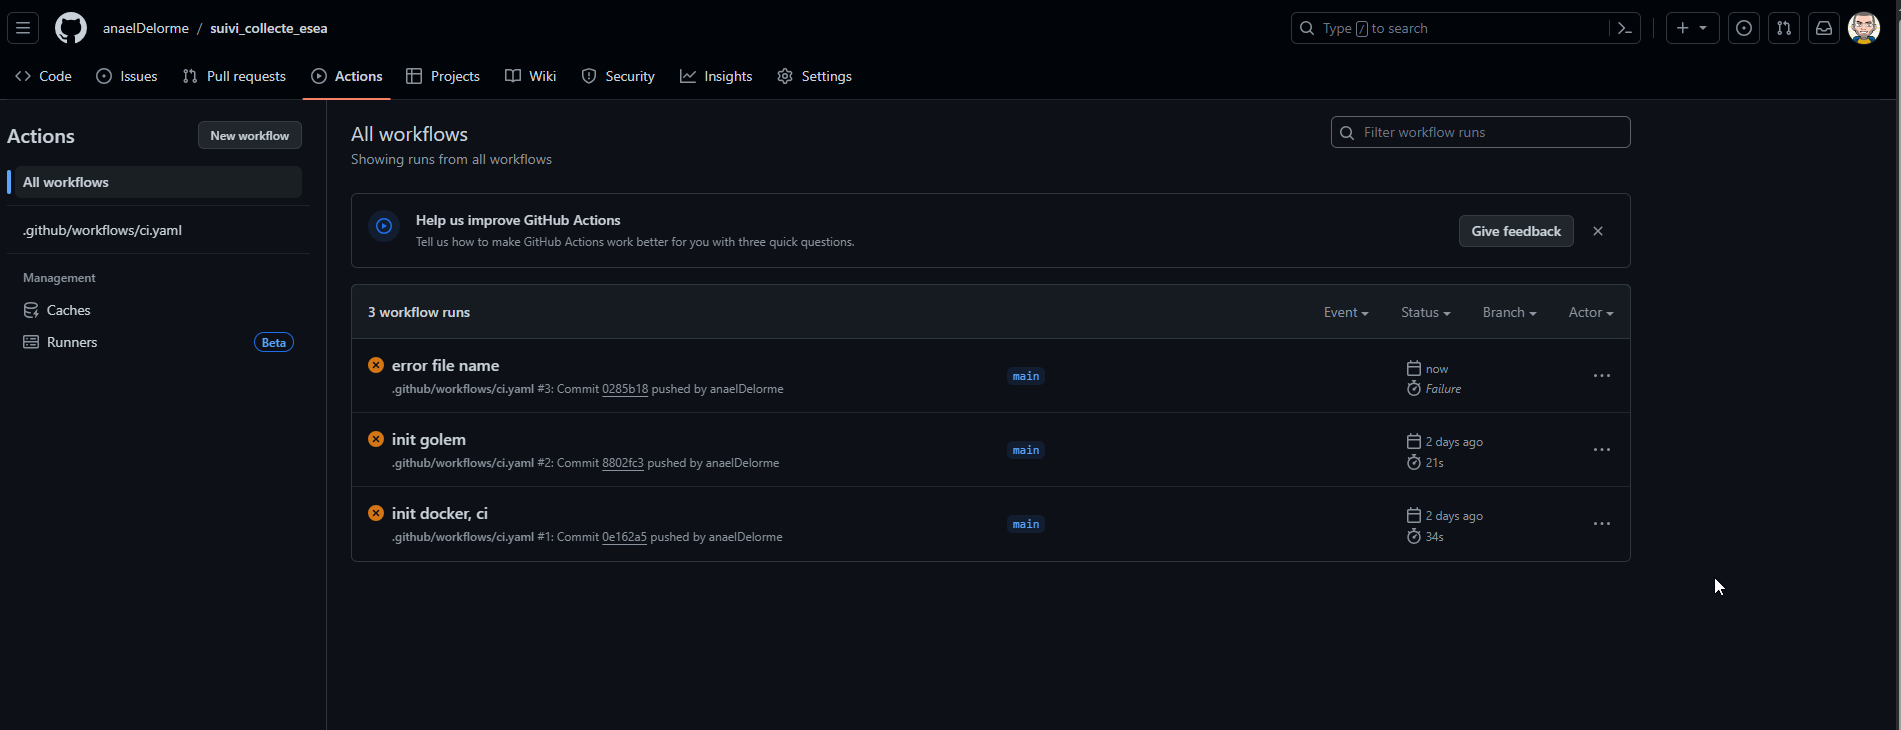
\includegraphics{./images/github_actions_error.png}

Si le workflow a bien fonctionné, vous aurez cela :

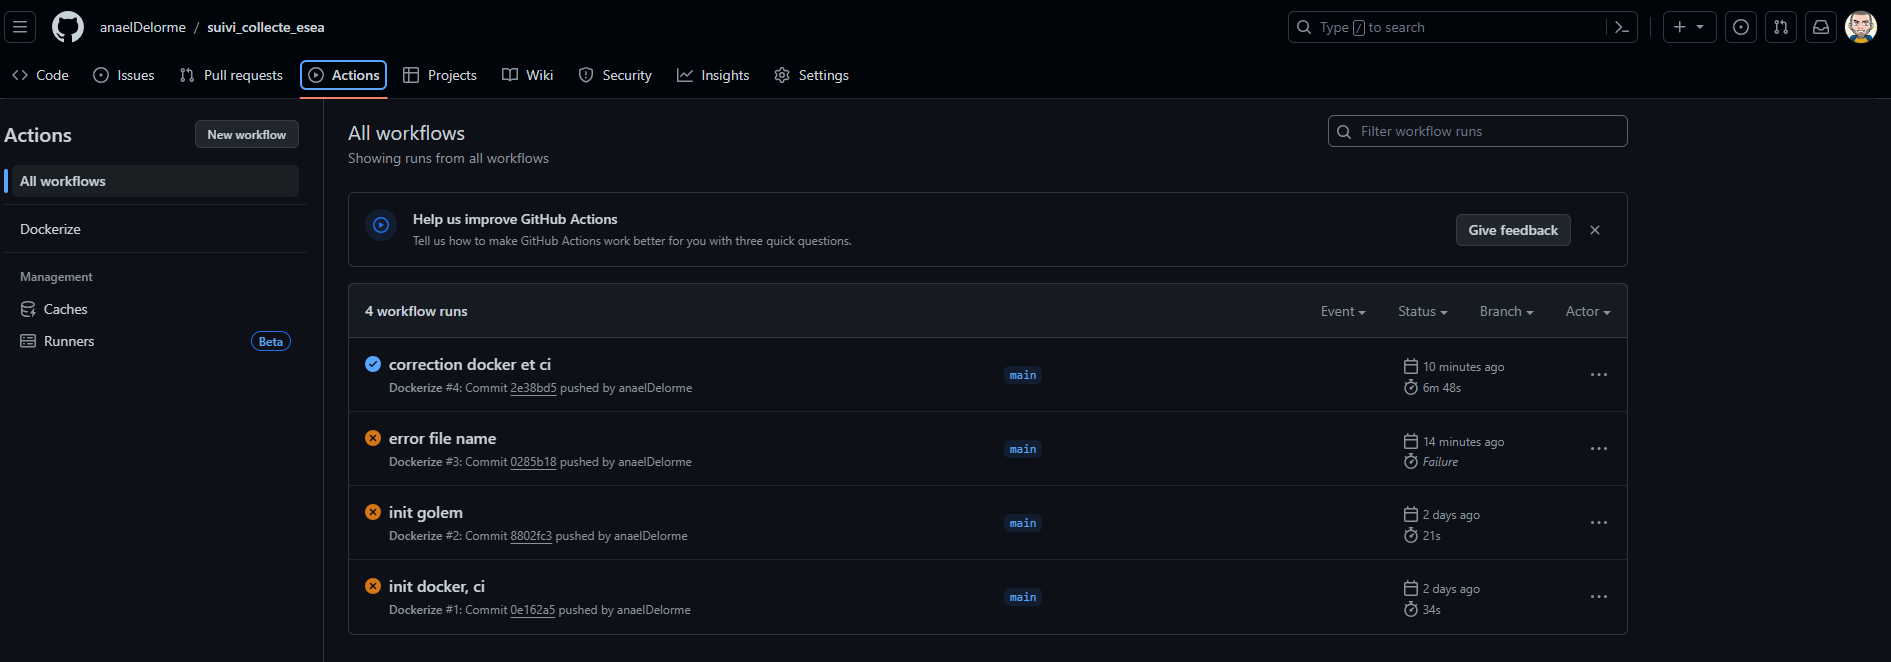
\includegraphics{./images/github_actions_ok.png}

Vous pouvez maintenant vérifier dans DockerHub que le Docker a bien été
déposé :

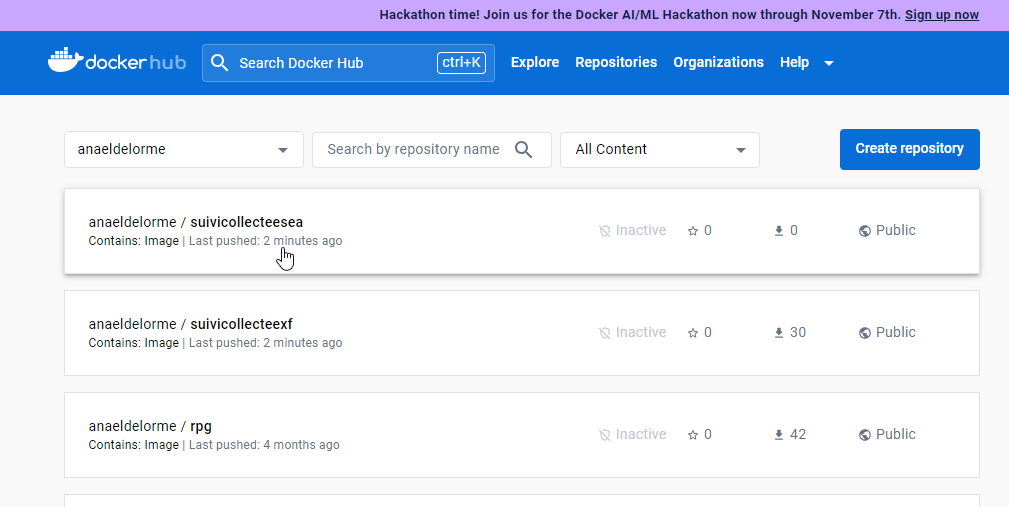
\includegraphics{./images/dockerhub_ok.png}

\hypertarget{gestion-du-duxe9ploiement}{%
\section{Gestion du déploiement}\label{gestion-du-duxe9ploiement}}

Notre Docker est sur DockerHub. Il ne reste plus qu'à l'installer sur le
datalab en passant par Chart Helm.

\hypertarget{cruxe9er-un-autre-repo-github-pour-guxe9rer-la-configuration-du-duxe9ploiement}{%
\subsection{Créer un autre repo github pour gérer la configuration du
déploiement}\label{cruxe9er-un-autre-repo-github-pour-guxe9rer-la-configuration-du-duxe9ploiement}}

Dans Github, créer un répertoire pour stocker les programmes permettant
le déploiement du site. Par exemple un répo :
\textbf{deploiemenetcollecteesea}. Copier le lien vers le repo

\hypertarget{cruxe9er-un-service-vscode-dans-le-datalab}{%
\subsection{Créer un service VScode dans le
datalab}\label{cruxe9er-un-service-vscode-dans-le-datalab}}

Dans le datalab, créez un nouveau service VSCode avec les droits d'admin
pour Kubernetes :

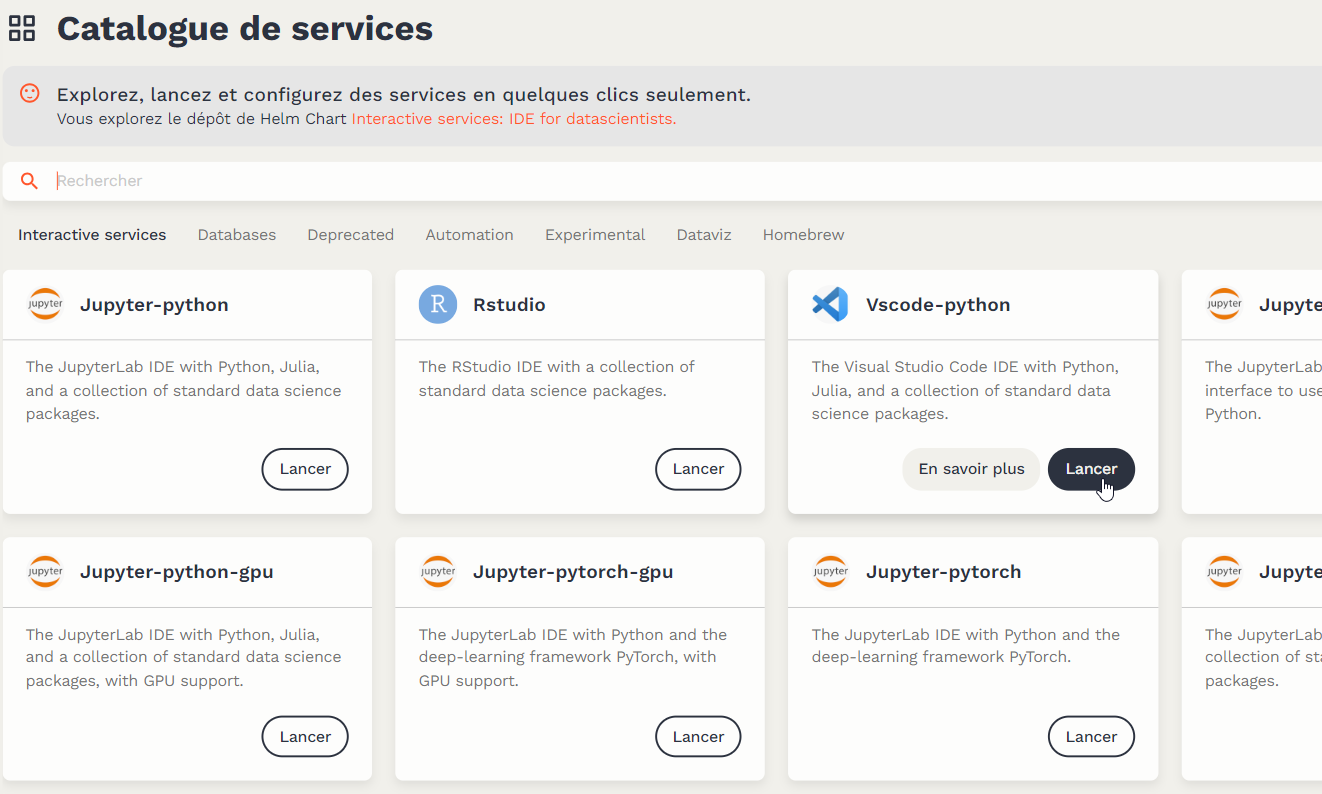
\includegraphics{./images/vscode_python.png}

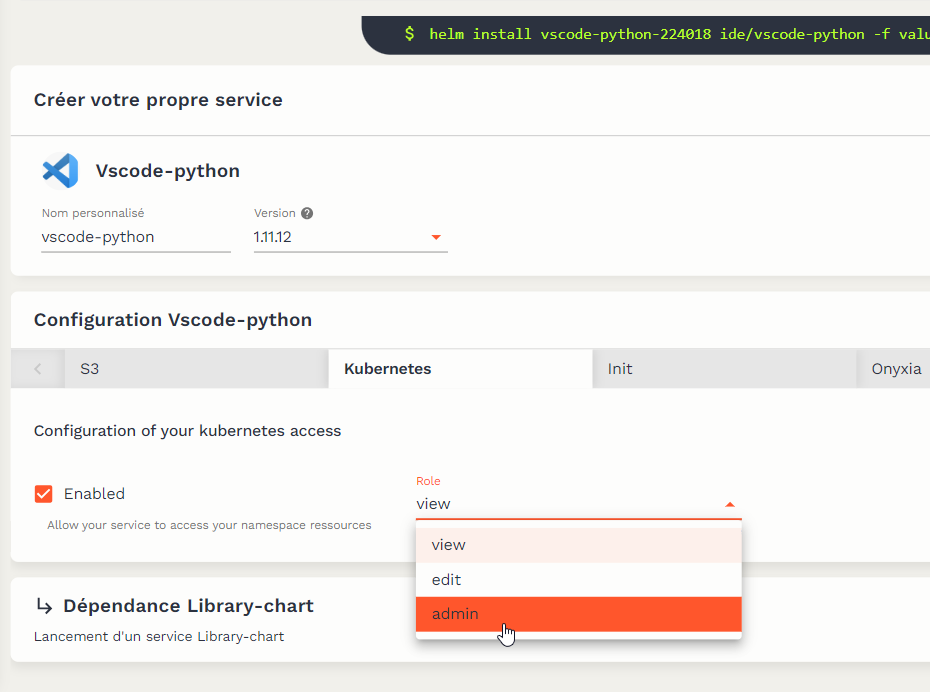
\includegraphics{./images/Vscode_kubernetes_admin.png}

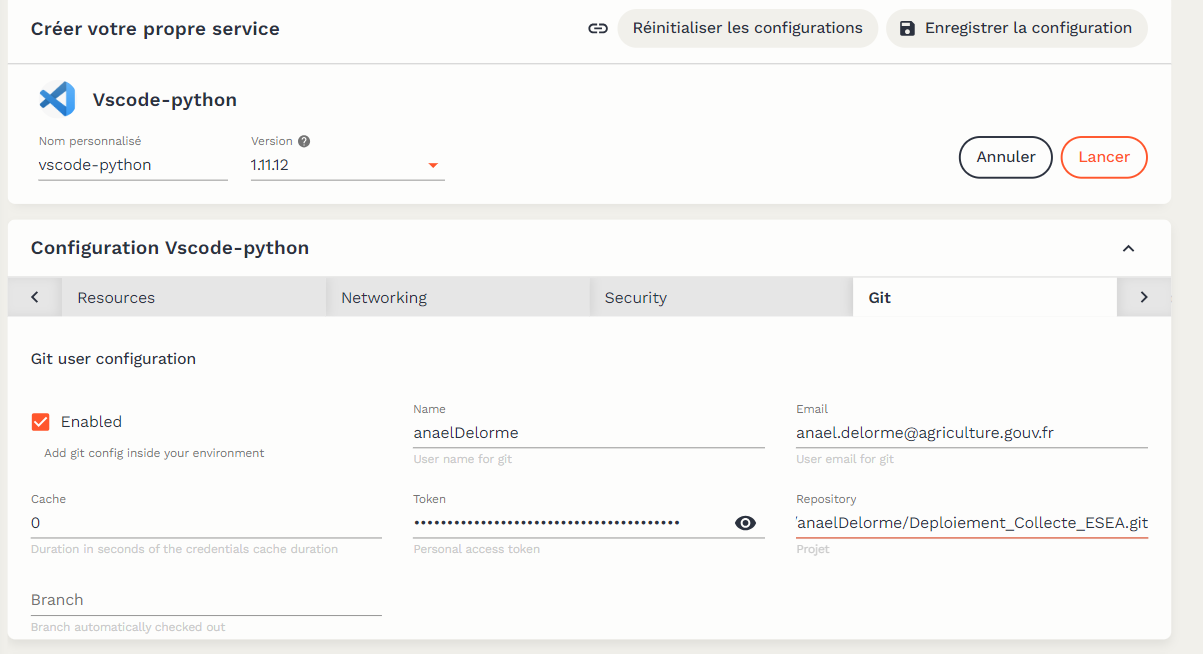
\includegraphics{./images/vscode_deplo_git.png}

\hypertarget{ajouter-les-fichiers-de-configuration}{%
\subsection{Ajouter les fichiers de
configuration}\label{ajouter-les-fichiers-de-configuration}}

Il faut ajouter 2 fichiers qui seront remontées à Github :

\begin{itemize}
\tightlist
\item
  Chart.yaml
\end{itemize}

Il faut modifier le nom du chart.

\begin{Shaded}
\begin{Highlighting}[]
\NormalTok{apiVersion: v2}
\NormalTok{name: suivi}\OperatorTok{{-}}\NormalTok{collecte}\OperatorTok{{-}}\NormalTok{esea}
\NormalTok{version: }\FloatTok{1.0.0}
\NormalTok{dependencies:}
  \OperatorTok{{-}}\NormalTok{ name: shiny}
\NormalTok{    version: }\FloatTok{1.0.0}
\NormalTok{    repository: https:}\OperatorTok{//}\NormalTok{inseefrlab.github.io}\OperatorTok{/}\NormalTok{helm}\OperatorTok{{-}}\NormalTok{charts}
\end{Highlighting}
\end{Shaded}

\begin{itemize}
\tightlist
\item
  values.yaml
\end{itemize}

Là il faut modifier le chemin et le nom du Docker sur DockerHub. Dans
ingress, on a l'url de notre site de suivi qui sera forcément de la
forme *.lab.sspcloud.fr.

Notez également l'existence de s3 et de existingSecret:
suivicollecteesea-s3. Nous allons le voir juste après.

\begin{Shaded}
\begin{Highlighting}[]
\NormalTok{shiny:}
\NormalTok{  image:}
\NormalTok{    repository: anaeldelorme}\OperatorTok{/}\NormalTok{suivicollecteesea}
\NormalTok{    tag: latest}
\NormalTok{    pullPolicy: Always}
\NormalTok{  ingress:}
\NormalTok{    enabled: true}
\NormalTok{    hostname: collecteesea.lab.sspcloud.fr}
\NormalTok{  s3:}
\NormalTok{    enabled: true}
\NormalTok{    existingSecret: suivicollecteesea}\OperatorTok{{-}}\NormalTok{s3}
\NormalTok{  resources: \{\}}
\end{Highlighting}
\end{Shaded}

\hypertarget{guxe9rer-les-secrets}{%
\subsection{Gérer les secrets}\label{guxe9rer-les-secrets}}

Notre application a accès aux données sur le s3 et gère des variables en
secret (identifiant / mot de passe du shinyManager). Pour gérer ces
variables sensibles, nous allons inscrire ces informations dans un objet
Kubernetes appelé Secret, qui va nous permettre de les passer à
l'application sous la forme de variables d'environnement.

Pour cela nous allons créer dans notre VSCode un troisième fichier que
nous n'allons pas importer dans Github. Créons ce fichier
\textbf{quelconque.yaml} et un fichier \textbf{.gitignore}. Dans le
fichier .gitignore, mettre uniquement quelconque.yaml. Cela indique
qu'il ignorera le fichier quelconque.yaml et ne le remontera pas sur
Github

Le fichier quelconque.yaml sera :

\begin{Shaded}
\begin{Highlighting}[]
\NormalTok{apiVersion: v1}
\NormalTok{kind: Secret}
\NormalTok{metadata:}
\NormalTok{  name: suivicollecteesea}\OperatorTok{{-}}\NormalTok{s3}
\BuiltInTok{type}\NormalTok{: Opaque}
\NormalTok{stringData:}
\NormalTok{  AWS\_ACCESS\_KEY\_ID: A CHANGER}
\NormalTok{  AWS\_SECRET\_ACCESS\_KEY: A CHANGER}
\NormalTok{  AWS\_S3\_ENDPOINT: minio.lab.sspcloud.fr}
\NormalTok{  AWS\_DEFAULT\_REGION: us}\OperatorTok{{-}}\NormalTok{east}\OperatorTok{{-}}\DecValTok{1}
\NormalTok{  LOGIN\_SITE\_1: A CHANGER}
\NormalTok{  MDP\_SITE\_1 : A CHANGER}
\NormalTok{  LOGIN\_SITE\_2: A CHANGER}
\NormalTok{  MDP\_SITE\_2 : A CHANGER}
\end{Highlighting}
\end{Shaded}

Concernant AWS\_ACCESS\_KEY\_ID et AWS\_SECRET\_ACCESS\_KEY, il faut
créer un ciompte de service sur la
\href{https://minio-console.lab.sspcloud.fr/login}{console Minio}. Pour
cela :

\begin{itemize}
\tightlist
\item
  menu ``Identity'' -\textgreater{} ``Service Accounts'' -\textgreater{}
  ``Create Service Account'' -\textgreater{} ``Create''\\
\item
  menu ``Access Keys'' -\textgreater{} ``Create access key''
\item
  comme précédemment, copier les informations de connexion dans votre
  quelconque.yaml
\end{itemize}

Pour LOGIN\_SITE\_1 / MDP\_SITE\_1, et les potentiels autres login/mdp,
vous spécifiez ici les différents logins/mots de passe que nous
fournirez à vos utilisateurs.

Quand le fichier est terminé, nous pouvez lancer dans un terminal du
Vscode (File --\textgreater{} Terminal --\textgreater{} New terminal) :
\textbf{kubectl apply -f deploiemenetcollecteesea/quelconque.yaml}

Si tout a bien fonctionné, un message devrait confirmer la création du
secret. Du style secret/nom\_de\_secret created où nom\_de\_secret est
ce que vous avez renseigné dans metadata.name du fichier
quelconque.yaml.

\hypertarget{lancer-le-duxe9ploiement}{%
\subsection{Lancer le déploiement}\label{lancer-le-duxe9ploiement}}

Dans le terminal, lancer : \textbf{helm dependency update
deploiemenetcollecteesea}. Puis \textbf{helm install
deploiemenetcollecteesea --generate-name}.

\hypertarget{vuxe9rifier-le-duxe9ploiement}{%
\subsection{Vérifier le
déploiement}\label{vuxe9rifier-le-duxe9ploiement}}

La première chose à vérifier c'est l'existence du helm en lançant :
\textbf{helm ls}. Il faut que le status soit à \textbf{deployed}.

\href{https://github.com/InseeFrLab/sspcloud-tutorials/blob/main/deployment/shiny-app.md}{Plus
d'infos sur la procédure de déploiement}

\bookmarksetup{startatroot}

\hypertarget{modifier-une-application-existante}{%
\chapter{Modifier une application
existante}\label{modifier-une-application-existante}}

\hypertarget{charger-les-nouvelles-donnuxe9es}{%
\section{Charger les nouvelles
données}\label{charger-les-nouvelles-donnuxe9es}}

Prérequis :

\begin{itemize}
\tightlist
\item
  avoir un compte sur le Datalab\\
\item
  ëtre membre du projet \textbf{projet-suivi-collecte-masa}
\end{itemize}

C'est très simple :

\begin{itemize}
\tightlist
\item
  télécharger les données d'export de Capibara\\
\item
  lancer le script de transformation en un fichier parquet (script qui
  permet d'enlever les données sensibles)\\
\item
  aller sur le \href{https://datalab.sspcloud.fr/}{datalab}
\item
  se connecter\\
\item
  aller sur Mes fichiers puis choisir le projet
  \textbf{projet-suivi-collecte-masa} :
  \href{https://datalab.sspcloud.fr/my-files/projet-suivi-collecte-masa}{lien
  direct}\\
\item
  choisir le répertoire de l'enquête\\
\item
  supprimer le(s) fichier(s) parquet\\
\item
  glisser/déposer le(s) nouveau(x) fichier(s) parquet
\end{itemize}

\hypertarget{modifier-le-site-de-suivi}{%
\section{Modifier le site de suivi}\label{modifier-le-site-de-suivi}}

\hypertarget{modifier-lapplication-rshiny}{%
\subsection{Modifier l'application
Rshiny}\label{modifier-lapplication-rshiny}}

Prérequis :

\begin{itemize}
\tightlist
\item
  avoir un compte sur le Datalab\\
\item
  avoir un compte Github\\
\item
  être collaborateur sur le repo Github du projet
\end{itemize}

Voici les étapes à suivre :

\begin{itemize}
\tightlist
\item
  aller \href{https://github.com/}{github}\\
\item
  se connecter\\
\item
  aller sur le repo du site de suivi : suivi-collecte-XXX\\
\item
  copier le lien pour cloner le repo :\\
  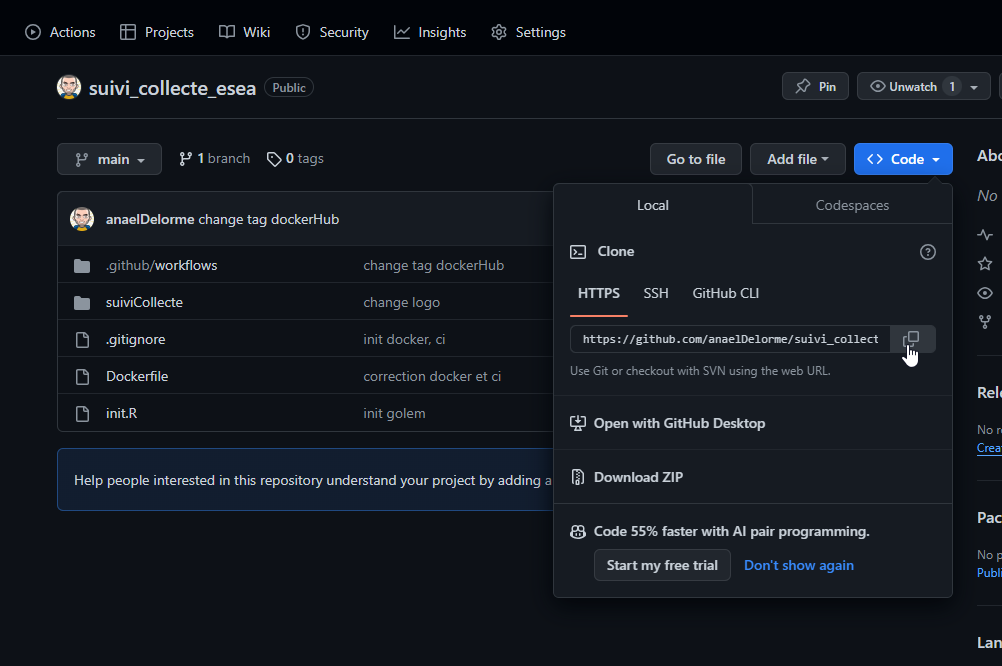
\includegraphics{./images/github_clone.png}\\
\item
  aller sur le \href{https://datalab.sspcloud.fr/}{datalab}\\
\item
  se connecter\\
\item
  créer un service VSCode-r-python-julia et indiquer le lien de clone du
  repo Github\\
  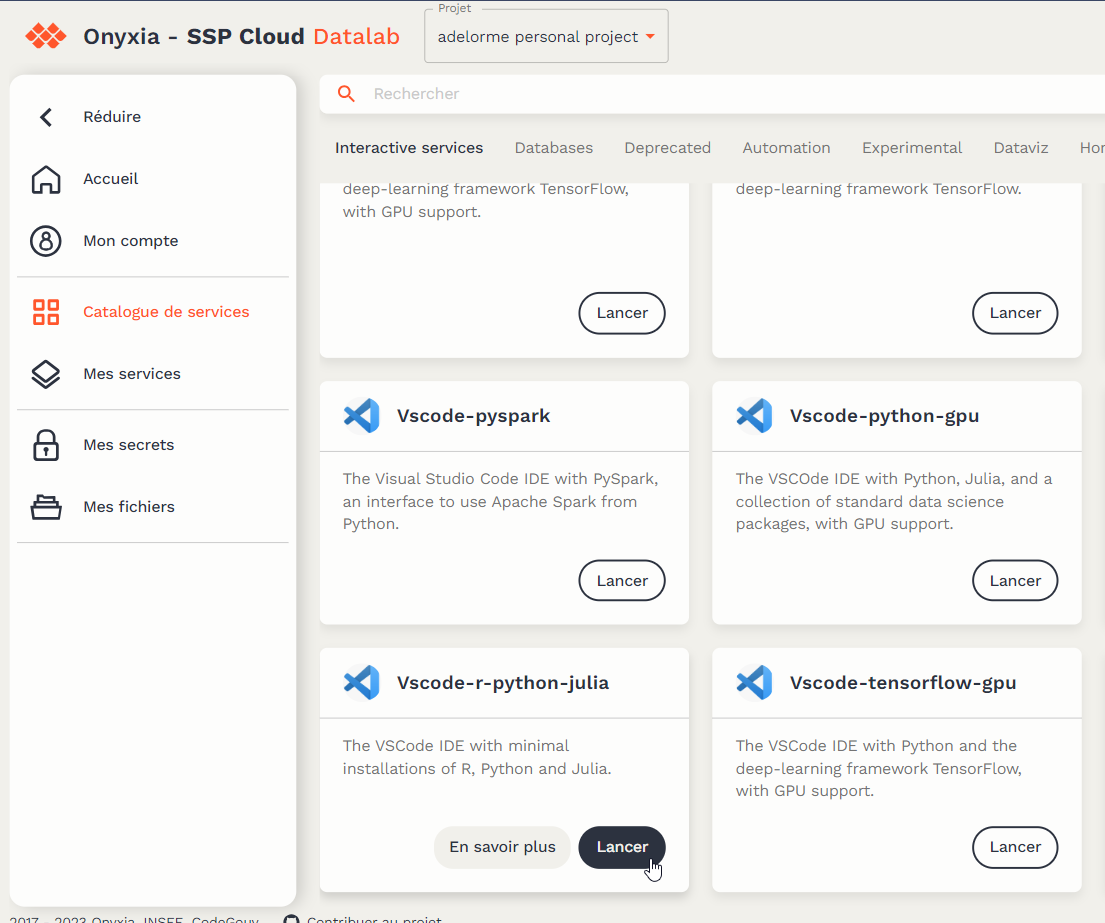
\includegraphics{./images/datalab_vscode_service.png}\\
  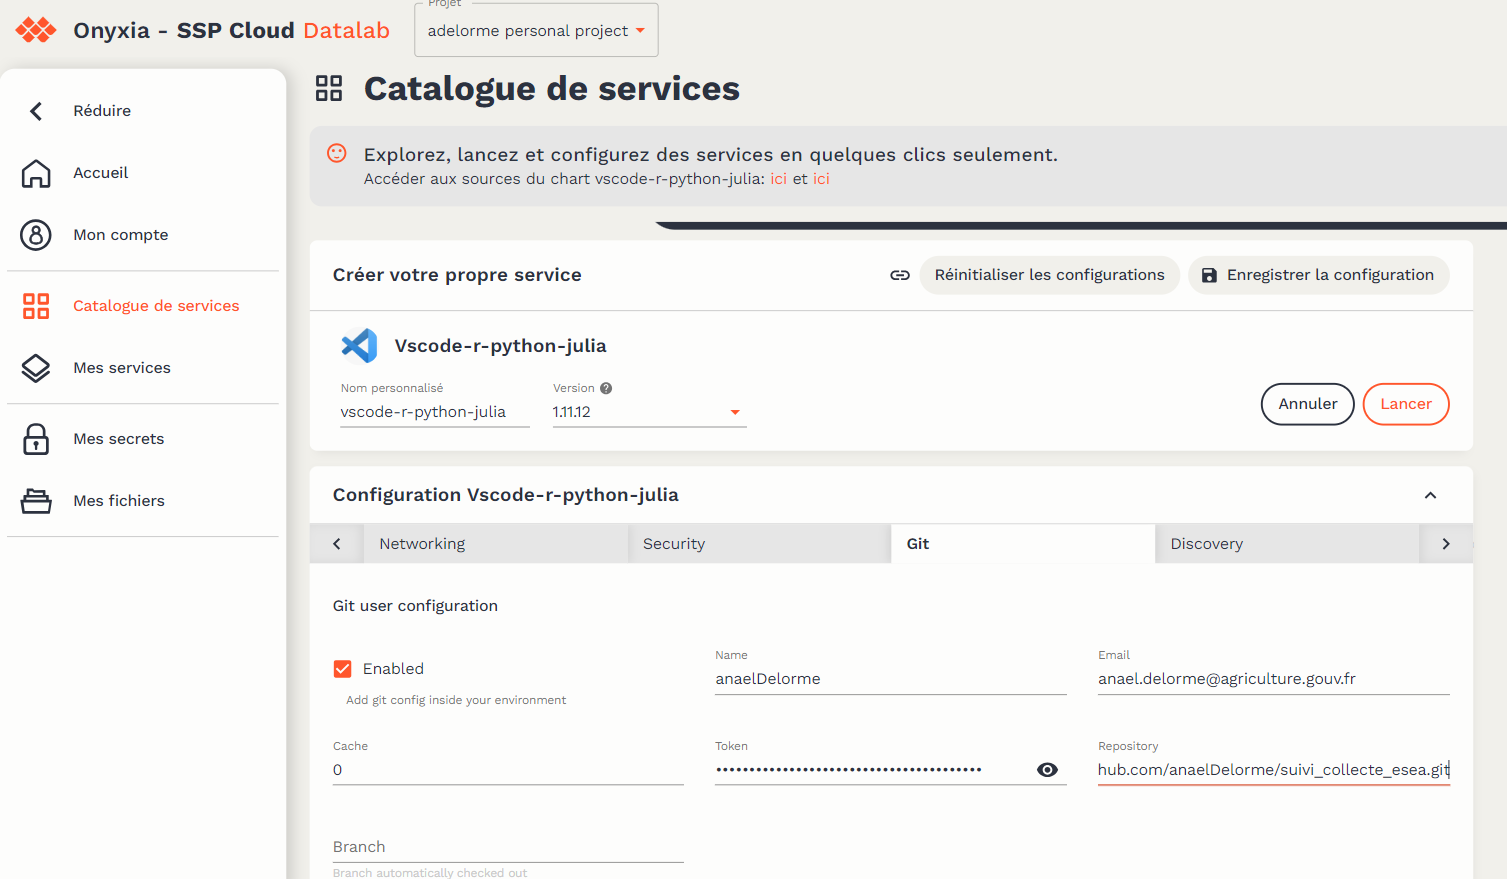
\includegraphics{./images/conf_git_vscode.png}\\
\item
  se connecter au service VSCode\\
\item
  ouvrir un nouveau terminal et coller la commande :
\end{itemize}

\begin{Shaded}
\begin{Highlighting}[]
\NormalTok{sudo apt}\OperatorTok{{-}}\NormalTok{get update}
\NormalTok{sudo apt}\OperatorTok{{-}}\NormalTok{get }\OperatorTok{{-}}\NormalTok{y install libudunits2}\OperatorTok{{-}}\NormalTok{dev}
\NormalTok{sudo apt}\OperatorTok{{-}}\NormalTok{get }\OperatorTok{{-}}\NormalTok{y install libproj}\OperatorTok{{-}}\NormalTok{dev}
\NormalTok{sudo apt}\OperatorTok{{-}}\NormalTok{get }\OperatorTok{{-}}\NormalTok{y install libgdal}\OperatorTok{{-}}\NormalTok{dev}
\NormalTok{sudo apt}\OperatorTok{{-}}\NormalTok{get install pandoc}
\end{Highlighting}
\end{Shaded}

\begin{itemize}
\tightlist
\item
  installer les packages utiles : taper r dans le terminal puis coller
  la commande suivante :
\end{itemize}

\begin{Shaded}
\begin{Highlighting}[]
\FunctionTok{install.packages}\NormalTok{(}\FunctionTok{c}\NormalTok{(}\StringTok{"tidyverse"}\NormalTok{, }\StringTok{"arrow"}\NormalTok{, }\StringTok{"shiny"}\NormalTok{, }\StringTok{"shinyWidgets"}\NormalTok{, }\StringTok{"bs4Dash"}\NormalTok{, }\StringTok{"shinymanager"}\NormalTok{, }\StringTok{"leaflet"}\NormalTok{, }\StringTok{"config"}\NormalTok{, }\StringTok{"DT"}\NormalTok{, }\StringTok{"echarts4r"}\NormalTok{, }\StringTok{"geojsonio"}\NormalTok{, }\StringTok{"glue"}\NormalTok{, }\StringTok{"golem"}\NormalTok{, }\StringTok{"htmlwidgets"}\NormalTok{, }\StringTok{"janitor"}\NormalTok{, }\StringTok{"sf"}\NormalTok{, }\StringTok{"testthat"}\NormalTok{, }\StringTok{"geojsonio"}\NormalTok{, }\StringTok{"dockerfiler"}\NormalTok{, }\StringTok{"attachment"}\NormalTok{, }\StringTok{"rsconnect"}\NormalTok{, }\StringTok{"spelling"}\NormalTok{, }\StringTok{"aws.s3"}\NormalTok{, }\StringTok{"waiter"}\NormalTok{, }\StringTok{"pandoc"}\NormalTok{))}
\end{Highlighting}
\end{Shaded}

\begin{itemize}
\tightlist
\item
  changer l'étiquette du docker pour indiquer que ce sera un nouvelle
  version :

  \begin{itemize}
  \tightlist
  \item
    ouvrir le fichier \textbf{.github/workflows/ci.yaml}\\
  \item
    ligne 38 changer la version
  \end{itemize}
\end{itemize}

\begin{Shaded}
\begin{Highlighting}[]
\CommentTok{\# Avant }
\AttributeTok{$\{\{ github.ref == \textquotesingle{}refs/heads/main\textquotesingle{} \&\& \textquotesingle{}anaeldelorme/suivicollecteesea:latest\textquotesingle{} \}\}}

\CommentTok{\# Après }
\AttributeTok{$\{\{ github.ref == \textquotesingle{}refs/heads/main\textquotesingle{} \&\& \textquotesingle{}anaeldelorme/suivicollecteesea:latest,anaeldelorme/suivicollecteesea:v1.0.0\textquotesingle{} \}\}}
\end{Highlighting}
\end{Shaded}

\begin{itemize}
\tightlist
\item
  indiquer la point de départ de l'application shiny :
  \textbf{setwd(``suivi\_collecte\_XXXXX/suiviCollecte/'')}\\
\item
  modifier l'application shiny en modifiant les pages, les box\ldots{}\\
\item
  si vous ajouter de nouveaux packages, pensez à les mettre dans un
  \textbf{\#' (\textbf{import?})}, puis lancez
  \textbf{attachment::att\_amend\_desc()}\\
\item
  tester l'application shiny en \emph{local} en faisant un lançant le
  fichier \textbf{dev/run\_dev.R}\\
\item
  vérifier que le package de l'application peut être créé en lançant un
  \textbf{devtools::check()}\\
\item
  s'il n'y a pas d'\textbf{errrors} dans le check, on peut alors
  committer et pusher dans Github\\
\item
  vérifier dans github que l'action s'est bien déroulée\\
\item
  vérifier que le Docker est bien accessible sur
  \href{https://hub.docker.com/}{Dockerhub}
\end{itemize}

NB : il est également possible de faire la même chose avec un Rstudio et
même en dehors du datalab. L'utilisation du Datalab est une meilleure
assurance que cela fonctionnera bien en déployant l'application (même
plateforme technique).

\hypertarget{duxe9ployer-la-nouvelle-version-de-lapplication}{%
\subsection{Déployer la nouvelle version de
l'application}\label{duxe9ployer-la-nouvelle-version-de-lapplication}}

Voici les étapes à suivre :

\begin{itemize}
\tightlist
\item
  aller \href{https://github.com/}{github}\\
\item
  se connecter\\
\item
  aller sur le repo de déploiement : deploiementcollecteXXXX
\item
  copier le lien pour cloner le repo :\\
  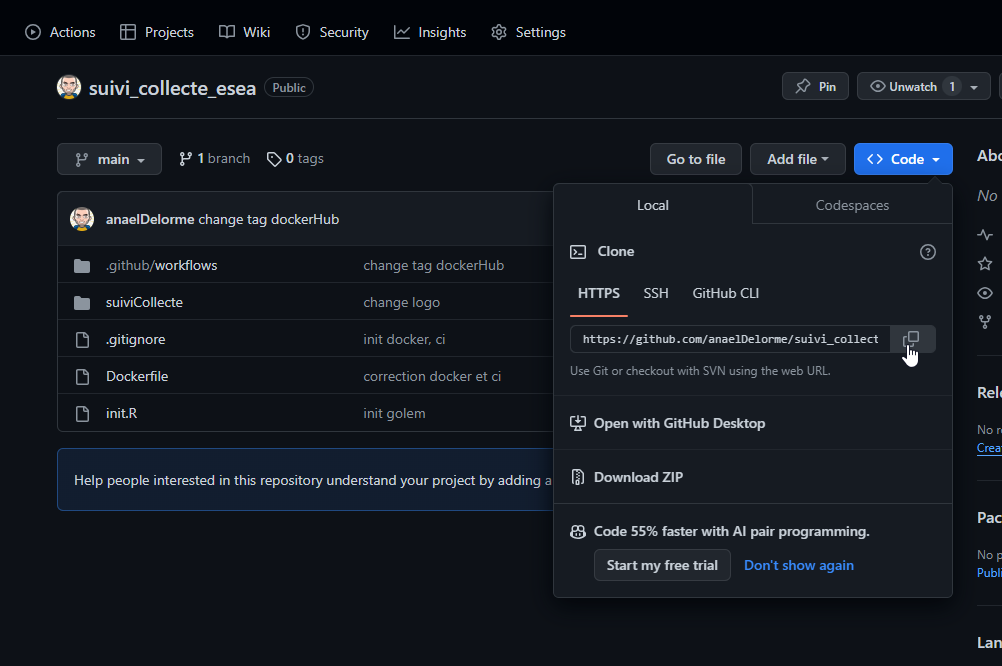
\includegraphics{./images/github_clone.png}\\
\item
  aller sur le \href{https://datalab.sspcloud.fr/}{datalab}\\
\item
  se connecter\\
\item
  créer un service VSCode-python, indiquer le lien de clone du repo
  Github et \textbf{mettre les droits d'admin Kubernetes}
  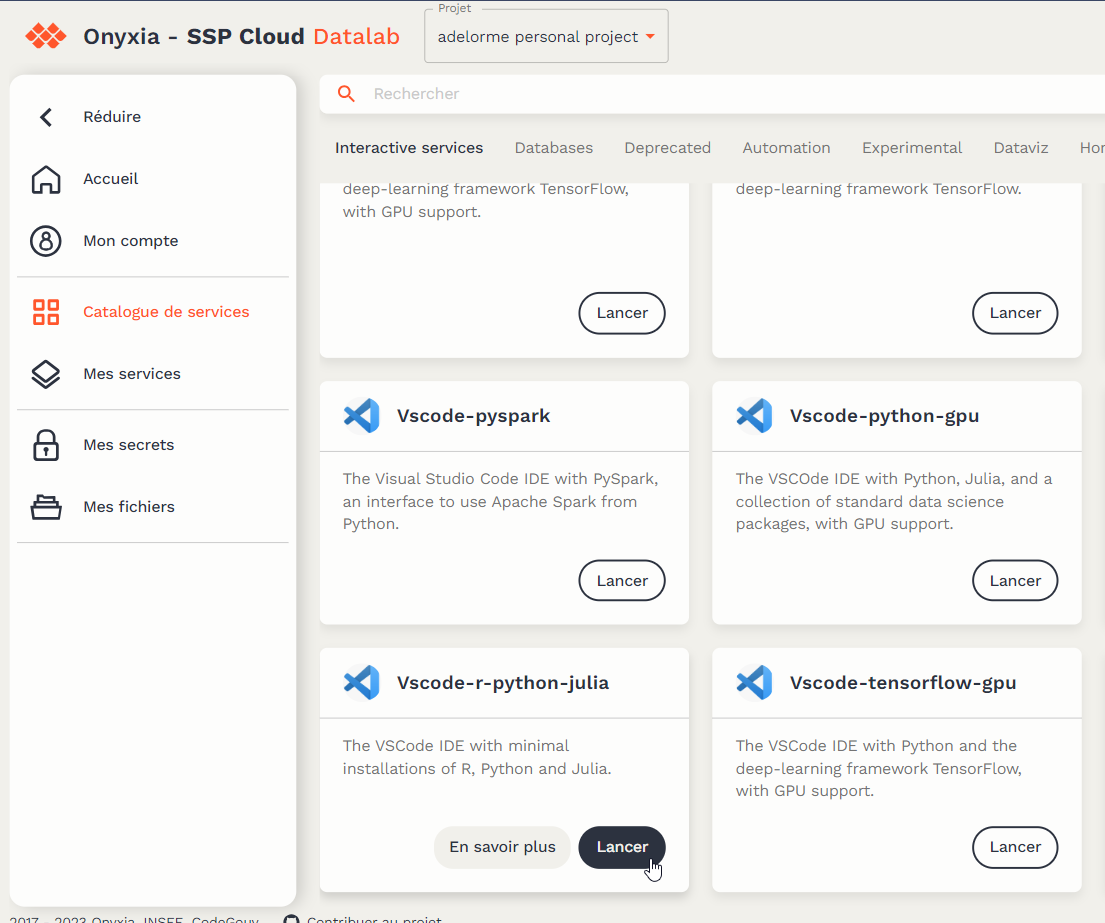
\includegraphics{./images/datalab_vscode_service.png}\\
  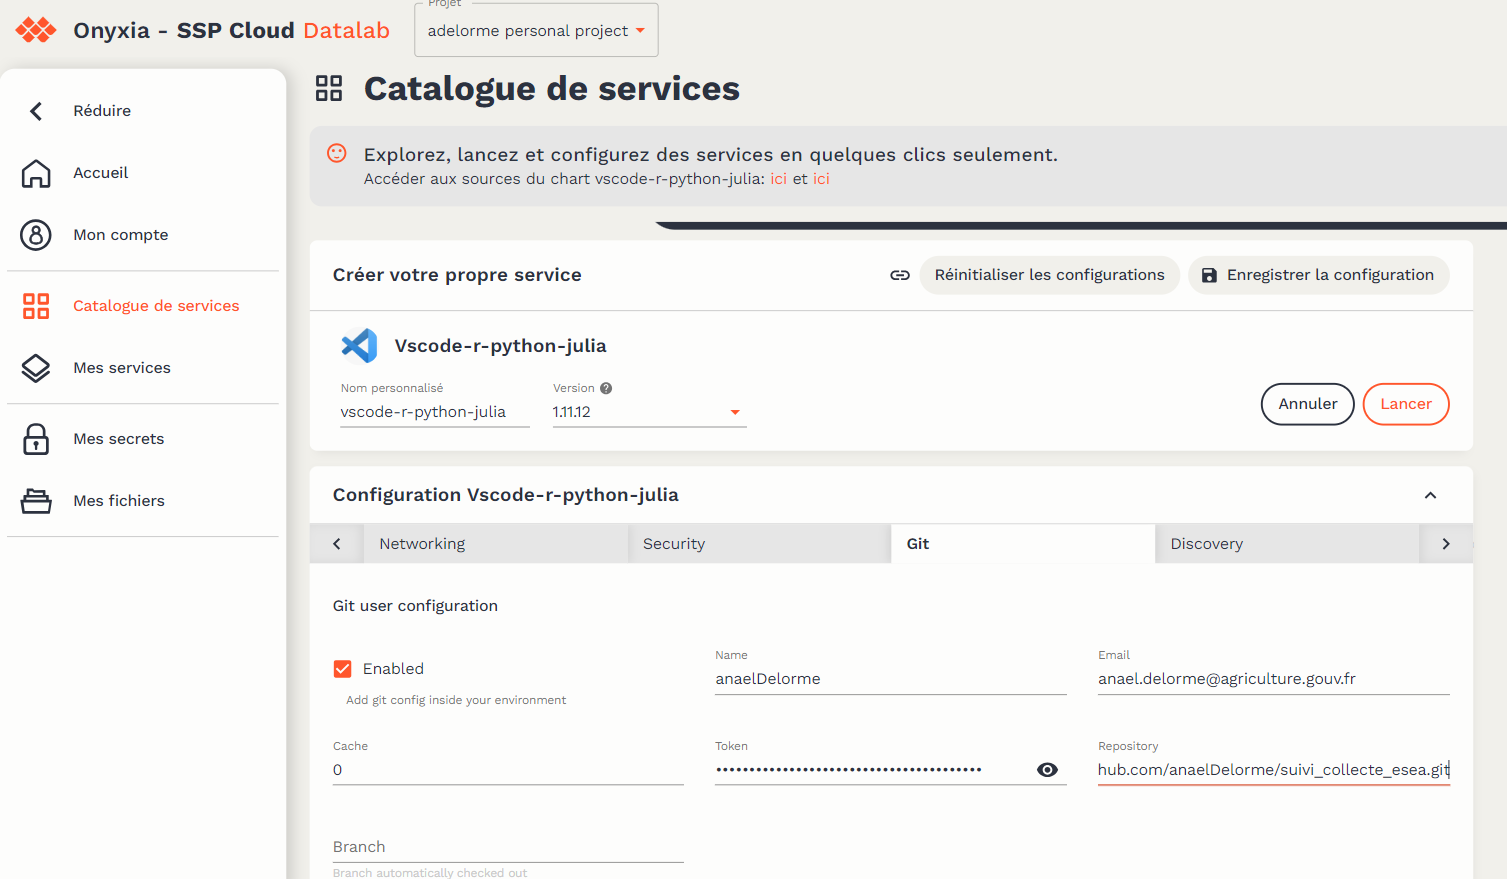
\includegraphics{./images/conf_git_vscode.png}\\
  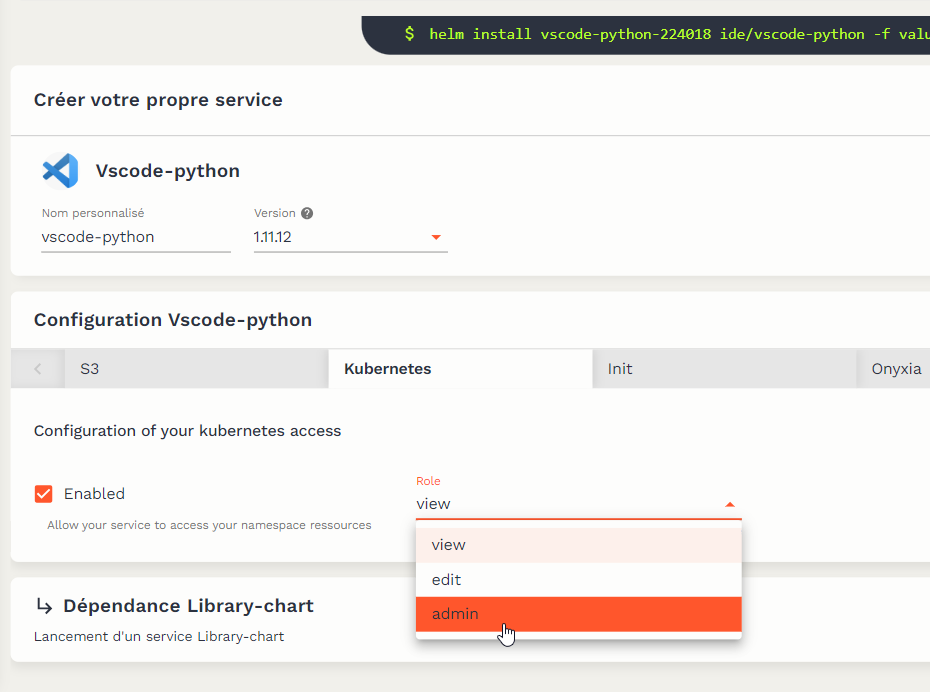
\includegraphics{./images/Vscode_kubernetes_admin.png}
\item
  se connecter au service VSCode\\
\item
  indiquer le tag de la version du Docker nouvellement créé dans le
  values.yaml à la 4ème ligne : \textbf{tag: v1.0.0}\\
\item
  dans le terminal saisir : \textbf{helm ls} pour trouver le nom du
  chart actuellement déployé\\
\item
  puis saisir : \textbf{helm dependency build
  deploiemenetcollecteXXXX/}\\
\item
  et enfin saisir \textbf{helm upgrade nom\_chart\_deploye
  deploiementcollecteXXXX/}
\end{itemize}

\bookmarksetup{startatroot}

\hypertarget{duxe9bugage-de-lapplication}{%
\chapter{Débugage de l'application}\label{duxe9bugage-de-lapplication}}

\hypertarget{vscode-pour-le-shiny-cannot-open-the-connection}{%
\section{VScode pour le shiny ``cannot open the
connection''}\label{vscode-pour-le-shiny-cannot-open-the-connection}}

Dans le développement de votre application, il se peut que vous
rencontriez cette erreur :

``cannot open the connectionwarning messages from top-level task
callback `vsc.workspace' Warning message: In file(con,''w'') : cannot
open file `/tmp/RtmpE07yck/vscode-R/workspace.json': No such file or
directory''

Cela peut arriver après une longue attente dans le service Vscode (par
exemple une nuit). Pour corriger, il faut commiter et pusher le code
dans github. Puis vous supprimez le service VSCode et vous recréez un
service VSCode en configurant le répertoire github. Pensez à lancer
l'installation les packages utiles. Il peut être utile de lancer dans le
terminal la commande
setwd(``/home/onyxia/work/suivi\_collecte\_XXXXX/suiviCollecte/'') pour
indiquer où trouver le projet Golem.

\bookmarksetup{startatroot}

\hypertarget{references}{%
\chapter*{References}\label{references}}
\addcontentsline{toc}{chapter}{References}

\hypertarget{refs}{}
\begin{CSLReferences}{0}{0}
\end{CSLReferences}



\printindex

\end{document}
